\documentclass[journal,12pt,twocolumn]{IEEEtran}
%
\usepackage{setspace}
\usepackage{gensymb}
%\doublespacing
\singlespacing

%\usepackage{graphicx}
%\usepackage{amssymb}
%\usepackage{relsize}
\usepackage[cmex10]{amsmath}
\usepackage{siunitx}
%\usepackage{amsthm}
%\interdisplaylinepenalty=2500
%\savesymbol{iint}
%\usepackage{txfonts}
%\restoresymbol{TXF}{iint}
%\usepackage{wasysym}
\usepackage{amsthm}
\usepackage{iithtlc}
\usepackage{mathrsfs}
\usepackage{txfonts}
\usepackage{stfloats}
\usepackage{steinmetz}
%\usepackage{bm}
\usepackage{cite}
\usepackage{cases}
\usepackage{subfig}
%\usepackage{xtab}
\usepackage{longtable}
\usepackage{multirow}
%\usepackage{algorithm}
%\usepackage{algpseudocode}
\usepackage{enumitem}
\usepackage{mathtools}
\usepackage{tikz}
\usepackage{circuitikz}
\usepackage{pgfplots}
\usepackage{verbatim}
\usepackage{tfrupee}
\usepackage[breaklinks=true]{hyperref}
%\usepackage{stmaryrd}
\usepackage{tkz-euclide} % loads  TikZ and tkz-base
%\usetkzobj{all}
\usetikzlibrary{calc,math}
\usetikzlibrary{fadings}
\usepackage{listings}
    \usepackage{color}                                            %%
    \usepackage{array}                                            %%
    \usepackage{longtable}                                        %%
    \usepackage{calc}                                             %%
    \usepackage{multirow}                                         %%
    \usepackage{hhline}                                           %%
    \usepackage{ifthen}                                           %%
  %optionally (for landscape tables embedded in another document): %%
    \usepackage{lscape}     
\usepackage{multicol}
\usepackage{chngcntr}
%\usepackage{enumerate}

%\usepackage{wasysym}
%\newcounter{MYtempeqncnt}
\DeclareMathOperator*{\Res}{Res}
%\renewcommand{\baselinestretch}{2}
\renewcommand\thesection{\arabic{section}}
\renewcommand\thesubsection{\thesection.\arabic{subsection}}
\renewcommand\thesubsubsection{\thesubsection.\arabic{subsubsection}}

\renewcommand\thesectiondis{\arabic{section}}
\renewcommand\thesubsectiondis{\thesectiondis.\arabic{subsection}}
\renewcommand\thesubsubsectiondis{\thesubsectiondis.\arabic{subsubsection}}

% correct bad hyphenation here
\hyphenation{op-tical net-works semi-conduc-tor}
\def\inputGnumericTable{}                                 %%

\lstset{
%language=C,
frame=single, 
breaklines=true,
columns=fullflexible
}
%\lstset{
%language=tex,
%frame=single, 
%breaklines=true
%}

\begin{document}
%


\newtheorem{theorem}{Theorem}[section]
\newtheorem{problem}{Problem}
\newtheorem{proposition}{Proposition}[section]
\newtheorem{lemma}{Lemma}[section]
\newtheorem{corollary}[theorem]{Corollary}
\newtheorem{example}{Example}[section]
\newtheorem{definition}[problem]{Definition}
%\newtheorem{thm}{Theorem}[section] 
%\newtheorem{defn}[thm]{Definition}
%\newtheorem{algorithm}{Algorithm}[section]
%\newtheorem{cor}{Corollary}
\newcommand{\BEQA}{\begin{eqnarray}}
\newcommand{\EEQA}{\end{eqnarray}}
\newcommand{\define}{\stackrel{\triangle}{=}}

\bibliographystyle{IEEEtran}
%\bibliographystyle{ieeetr}


\providecommand{\mbf}{\mathbf}
\providecommand{\pr}[1]{\ensuremath{\Pr\left(#1\right)}}
\providecommand{\qfunc}[1]{\ensuremath{Q\left(#1\right)}}
\providecommand{\sbrak}[1]{\ensuremath{{}\left[#1\right]}}
\providecommand{\lsbrak}[1]{\ensuremath{{}\left[#1\right.}}
\providecommand{\rsbrak}[1]{\ensuremath{{}\left.#1\right]}}
\providecommand{\brak}[1]{\ensuremath{\left(#1\right)}}
\providecommand{\lbrak}[1]{\ensuremath{\left(#1\right.}}
\providecommand{\rbrak}[1]{\ensuremath{\left.#1\right)}}
\providecommand{\cbrak}[1]{\ensuremath{\left\{#1\right\}}}
\providecommand{\lcbrak}[1]{\ensuremath{\left\{#1\right.}}
\providecommand{\rcbrak}[1]{\ensuremath{\left.#1\right\}}}
\theoremstyle{remark}
\newtheorem{rem}{Remark}
\newcommand{\sgn}{\mathop{\mathrm{sgn}}}
\providecommand{\abs}[1]{\left\vert#1\right\vert}
\providecommand{\res}[1]{\Res\displaylimits_{#1}} 
\providecommand{\norm}[1]{\left\lVert#1\right\rVert}
%\providecommand{\norm}[1]{\lVert#1\rVert}
\providecommand{\mtx}[1]{\mathbf{#1}}
\providecommand{\mean}[1]{E\left[ #1 \right]}
\providecommand{\fourier}{\overset{\mathcal{F}}{ \rightleftharpoons}}
%\providecommand{\hilbert}{\overset{\mathcal{H}}{ \rightleftharpoons}}
\providecommand{\ztrans}{\overset{\mathcal{Z}}{ \rightleftharpoons}}
\providecommand{\system}{\overset{\mathcal{H}}{ \longleftrightarrow}}
	%\newcommand{\solution}[2]{\textbf{Solution:}{#1}}
\newcommand{\solution}{\noindent \textbf{Solution: }}
\newcommand{\cosec}{\,\text{cosec}\,}
\providecommand{\dec}[2]{\ensuremath{\overset{#1}{\underset{#2}{\gtrless}}}}
\newcommand{\myvec}[1]{\ensuremath{\begin{pmatrix}#1\end{pmatrix}}}
\newcommand{\mydet}[1]{\ensuremath{\begin{vmatrix}#1\end{vmatrix}}}
\providecommand{\gauss}[2]{\mathcal{N}\ensuremath{\left(#1,#2\right)}}
%\providecommand{\system}[1]{\overset{\mathcal{#1}}{ \longleftrightarrow}}
\newcommand*{\permcomb}[4][0mu]{{{}^{#3}\mkern#1#2_{#4}}}
\newcommand*{\perm}[1][-3mu]{\permcomb[#1]{P}}
\newcommand*{\comb}[1][-1mu]{\permcomb[#1]{C}}
%\numberwithin{equation}{section}
\numberwithin{equation}{subsection}
%\numberwithin{problem}{section}
%\numberwithin{definition}{section}
\makeatletter
\@addtoreset{figure}{problem}
\makeatother

\let\StandardTheFigure\thefigure
\let\vec\mathbf
%\renewcommand{\thefigure}{\theproblem.\arabic{figure}}
\renewcommand{\thefigure}{\theproblem}
%\setlist[enumerate,1]{before=\renewcommand\theequation{\theenumi.\arabic{equation}}
%\counterwithin{equation}{enumi}


%\renewcommand{\theequation}{\arabic{subsection}.\arabic{equation}}

\def\putbox#1#2#3{\makebox[0in][l]{\makebox[#1][l]{}\raisebox{\baselineskip}[0in][0in]{\raisebox{#2}[0in][0in]{#3}}}}
     \def\rightbox#1{\makebox[0in][r]{#1}}
     \def\centbox#1{\makebox[0in]{#1}}
     \def\topbox#1{\raisebox{-\baselineskip}[0in][0in]{#1}}
     \def\midbox#1{\raisebox{-0.5\baselineskip}[0in][0in]{#1}}

\vspace{3cm}

\title{
%	\logo{
Probability and Random Variables
%	}
}
\author{ G V V Sharma$^{*}$% <-this % stops a space
	\thanks{*The author is with the Department
		of Electrical Engineering, Indian Institute of Technology, Hyderabad
		502285 India e-mail:  gadepall@iith.ac.in. All content in this manual is released under GNU GPL.  Free and open source.}
	
}	
%\title{
%	\logo{Matrix Analysis through Octave}{\begin{center}\includegraphics[scale=.24]{tlc}\end{center}}{}{HAMDSP}
%}


% paper title
% can use linebreaks \\ within to get better formatting as desired
%\title{Matrix Analysis through Octave}
%
%
% author names and IEEE memberships
% note positions of commas and nonbreaking spaces ( ~ ) LaTeX will not break
% a structure at a ~ so this keeps an author's name from being broken across
% two lines.
% use \thanks{} to gain access to the first footnote area
% a separate \thanks must be used for each paragraph as LaTeX2e's \thanks
% was not built to handle multiple paragraphs
%

%\author{<-this % stops a space
%\thanks{}}
%}
% note the % following the last \IEEEmembership and also \thanks - 
% these prevent an unwanted space from occurring between the last author name
% and the end of the author line. i.e., if you had this:
% 
% \author{....lastname \thanks{...} \thanks{...} }
%                     ^------------^------------^----Do not want these spaces!
%
% a space would be appended to the last name and could cause every name on that
% line to be shifted left slightly. This is one of those "LaTeX things". For
% instance, "\textbf{A} \textbf{B}" will typeset as "A B" not "AB". To get
% "AB" then you have to do: "\textbf{A}\textbf{B}"
% \thanks is no different in this regard, so shield the last } of each \thanks
% that ends a line with a % and do not let a space in before the next \thanks.
% Spaces after \IEEEmembership other than the last one are OK (and needed) as
% you are supposed to have spaces between the names. For what it is worth,
% this is a minor point as most people would not even notice if the said evil
% space somehow managed to creep in.



% The paper headers
%\markboth{Journal of \LaTeX\ Class Files,~Vol.~6, No.~1, January~2007}%
%{Shell \MakeLowercase{\textit{et al.}}: Bare Demo of IEEEtran.cls for Journals}
% The only time the second header will appear is for the odd numbered pages
% after the title page when using the twoside option.
% 
% *** Note that you probably will NOT want to include the author's ***
% *** name in the headers of peer review papers.                   ***
% You can use \ifCLASSOPTIONpeerreview for conditional compilation here if
% you desire.




% If you want to put a publisher's ID mark on the page you can do it like
% this:
%\IEEEpubid{0000--0000/00\$00.00~\copyright~2007 IEEE}
% Remember, if you use this you must call \IEEEpubidadjcol in the second
% column for its text to clear the IEEEpubid mark.



% make the title area
\maketitle

\newpage

\tableofcontents

\bigskip

\renewcommand{\thefigure}{\theenumi}
\renewcommand{\thetable}{\theenumi}
%\renewcommand{\theequation}{\theenumi}

%\begin{abstract}
%%\boldmath
%In this letter, an algorithm for evaluating the exact analytical bit error rate  (BER)  for the piecewise linear (PL) combiner for  multiple relays is presented. Previous results were available only for upto three relays. The algorithm is unique in the sense that  the actual mathematical expressions, that are prohibitively large, need not be explicitly obtained. The diversity gain due to multiple relays is shown through plots of the analytical BER, well supported by simulations. 
%
%\end{abstract}
% IEEEtran.cls defaults to using nonbold math in the Abstract.
% This preserves the distinction between vectors and scalars. However,
% if the journal you are submitting to favors bold math in the abstract,
% then you can use LaTeX's standard command \boldmath at the very start
% of the abstract to achieve this. Many IEEE journals frown on math
% in the abstract anyway.

% Note that keywords are not normally used for peerreview papers.
%\begin{IEEEkeywords}
%Cooperative diversity, decode and forward, piecewise linear
%\end{IEEEkeywords}



% For peer review papers, you can put extra information on the cover
% page as needed:
% \ifCLASSOPTIONpeerreview
% \begin{center} \bfseries EDICS Category: 3-BBND \end{center}
% \fi
%
% For peerreview papers, this IEEEtran command inserts a page break and
% creates the second title. It will be ignored for other modes.
%\IEEEpeerreviewmaketitle

\begin{abstract}
This book provides a simple introduction to probability and random variables.   The contents are largely based on  NCERT textbooks from Class 9-12.
\end{abstract}


\section{Axioms of Probability}

\renewcommand{\theequation}{\theenumi}
\begin{enumerate}[label=\thesection.\arabic*.,ref=\thesection.\theenumi]
\numberwithin{equation}{enumi}

\item Which of the following cannot be the probability of an event?\\
(A)$\frac{2}{3}$(B) –1.5 (C) 15 (D) 0.7
\\
\solution $0 < \pr{E} < 1$.  Hence, (B) and (C) are the right answer.
\item If P(E) = 0.05, what is the probability of ‘not E’?
%
\solution 
The desired probability is
\begin{align}
\pr{E^{\prime}} = 1 - \pr{E} = 0.95
\end{align}
%
\item If A and B are two events such that P(A) $\neq$ 0 and P(B/A) = 1, then
(A) A $\subset$ B \\
(B) B $\subset$ A \\
(C) B = $\phi$ \\
(D) A = $\phi$\\
\solution
Given 
\begin{align}
Pr(B | A)=1. 
\end{align}
By definition,
\begin{align}
Pr(B|A)=\frac{Pr(AB)}{Pr(A)}
\end{align}
\begin{align}
&\implies\frac{Pr(AB)}{Pr(A)} = 1\\
&\implies Pr(AB) = Pr(A)\label{1}\\
&\implies AB= A\label{2}
\end{align}
\begin{enumerate}[label={\Alph*)}]
\item Take any 
\begin{align}
    X \in A
\end{align} . From \eqref{2}, we get
\begin{align}
     X \in AB
\end{align}is also true.\\
Therefore, for any 
\begin{align}
  X \in A \\
  \implies X \in B   
\end{align}
    \begin{align}
     A \subseteq B 
\end{align}is also true.\\
    But, since A and B are two events,
    \begin{align}
       A\neq B 
    \end{align}. Hence,
    \begin{align}
    A \subset B
\end{align}
Therefore, option (A) is correct.
% \begin{figure}[h]
%     \centering
%     \includegraphics[width=8cm]{venn.png}
    
%     \label*{Venn diagram}
% \end{figure}
\item If 
\begin{align}
  B \subset A  
\end{align}
Then, 
\begin{align}
AB=B.
\end{align}
\begin{align}
\implies Pr(AB)=Pr(B)
\end{align}
But, from \eqref{1}, we have, 
\begin{align}
&Pr(AB)=Pr(A)\\
\implies &Pr(AB)=Pr(A)=Pr(B)
\end{align}
But,since A and B are two events, 
\begin{align}
    A\neq B
\end{align}. Hence, option (B) is incorrect.
 \item If 
 \begin{align}
     B=\phi
 \end{align}
\begin{align}
\implies Pr(AB)=0
\end{align}From \eqref{1}, we know that,
\begin{align}
& Pr(AB)=Pr(A)\\
\implies & Pr(AB)=Pr(A)=0
\end{align}
But,from the given data, we know that 
\begin{align}
     Pr(A) \neq 0
 \end{align}
Therefore,option C is incorrect.
\item If 
\begin{align}
     A=\phi
 \end{align}
\begin{align}
\implies Pr(A)=0
\end{align}
But,from the given data, we know that 
\begin{align}
     Pr(A) \neq 0
 \end{align}
Therefore,option D is incorrect.
\end{enumerate}

\item If P(A/B) $>$ P(A), then which of the following is correct :
(A) P(B/A) $<$ P(B) \\
(B) P(A $\cap$ B) $<$ P(A) . P(B)\\
(C) P(B/A) $>$ P(B) \\
(D) P(B/A) = P(B)
\solution
From the given information,
\begin{align}
    \label{eq:6.4.1}
    \frac{\pr{AB}}{\pr{B}}>\pr{A}\\
    \label{eq:6.4.2}
    \implies \pr{AB}>\pr{A}.\pr{B}
\end{align}
Hence, option (B) is false. Now, dividing the equation by \pr{A} on both sides i.e.,
\begin{align}
    \label{eq:6.4.3}
    \frac{\pr{AB}}{\pr{A}}>\pr{B}   
\end{align}
But $\frac{\pr{AB}}{\pr{A}}$ = \pr{B|A}. Therefore, from     \eqref{eq:6.4.3}
\begin{align}
    \label{eq:6.4.4}
    \pr{B|A}>\pr{B}
\end{align}
Hence, option (C) is correct.


\item If A and B are any two events such that P(A) + P(B) – P(A and B) = P(A), then\\
(A) P(B/A) = 1 \\
(B) P(A/B) = 1\\
(C) P(B/A) = 0 \\
(D) P(A/B) = 0\\
\item Complete the following statements:\\
 (i) Probability of an event E + Probability of the event ‘not E’ =----------- .\\
 (ii) The probability of an event that cannot happen is---------- . Such an event is called--------- .\\
 (iii) The probability of an event that is certain to happen is ---------.\\
 (iv) The sum of the probabilities of all the elementary events of an experiment is----------.\\ 
 (v) The probability of an event is greater than or equal to and less than or equal to --------------.\\
 %
 \solution
 \begin{enumerate}
 \item 1
 \item 0, null
 \item 1
 \item 1
 \item $0 \le \pr{E} \le 1$.
 \end{enumerate}
 \item An electronic assembly consists of two subsystems, say, A and B. From previous testing procedures, the following probabilities are assumed to be known:\\
P(A fails) = 0.2\\
P(B fails alone) = 0.15\\
P(A and B fail) = 0.15\\
\\Evaluate the following probabilities\\
(i) P(A fails|B has failed) \\
(ii) P(A fails alone)\\
\item A and B are two events such that P (A) $\neq$ 0. Find P(B/A), if\\
(i) A is a subset of B \\
(ii) A $\cap$ B = $\phi$\\
\solution
By definition,
%
\begin{align}
\pr{B|A} = \frac{\pr{AB}}{\pr{A}} 
\label{eq:axioms_6.8}
\end{align}
%
\begin{enumerate}
\item
\begin{align}
A &\subset B \implies \pr{AB} = \pr{A}
\\
\implies \pr{B|A} &= 1
\end{align}
%
upon substituting in \eqref{eq:axioms_6.8}
\item
\begin{align}
A \cup B = \phi \implies \pr{AB} = 0
\\
\implies \pr{B|A} &= 0
\end{align}
%
upon substituting in \eqref{eq:axioms_6.8}
\end{enumerate}
\item If A and B are two events such that A $\subset$ B and P(B) $\neq$ 0, then which of the following is correct?\\
\begin{enumerate}
\item P(A/B) = $\frac{P(B)}{P(A)}$
\item $P(A/B) < P(A)$
\item P(A/B) $\geq$ P(A)
\item None of these
\end{enumerate}
\item Let E and F be events with $\pr{E} = \frac{3}{5}$, $\pr{F} = \frac{3}{10}$ and  $\pr{E \cap F} = \frac{1}{5}$. Are E and F independent?
\\
\solution 
\begin{align}
\pr{E}\pr{F} = \frac{9}{50} \ne \pr{E \cap F}
\end{align}
%
Hence E and F are not independent.
\item Given that the events A and B are such that P(A) = $\frac{1}{2}$, P(A $\cup B$)= $\frac{3}{5}$ and P(B) = p. Find p if they are\\
(i) mutually exclusive\\
(ii) independent.\\

\item Let A and B be independent events with P(A) = 0.3 and P(B) = 0.4. Find\\
(i) P(A $\cap$ B)\\ 
(ii) P(A $\cup$ B)\\
(iii) P(A/B)\\
(iv) P(B/A)\\

\item If A and B are two events such that P(A) = $\frac{1}{4}$, P(B) = $\frac{1}{2}$ and P(A $\cap$ B) = $\frac{1}{8}$. find P (not A and not B).\\

\item Events A and B are such that P (A) = $\frac{1}{2}$, P(B) = $\frac{7}{12}$ and P(not A or not B) = $\frac{1}{4}$. State whether A and B are independent ?\\

\item Given two independent events A and B such that P(A) = 0.3, P(B) = 0.6. Find\\
(i) P(A and B)\\
(ii) P(A and not B)\\
(iii) P(A or B)\\
(iv) P(neither A nor B)\\
%
\solution
\begin{enumerate}[label={\roman*)}]
\item
Since the events A and B are independent events, by definition
\begin{align}
    \pr{A\, and\, B} = \pr{AB}= \pr{A}\pr{B}\label{6.15:a}
\end{align}
On substituting the values of \pr{A},\pr{B} in \eqref{6.15:a}, we get
\begin{align}
    \pr{A\, and\, B} &= \pr{A}\pr{B}\\
    &= (0.3)(0.6)\\
    \implies \pr{A\, and\, B}&=0.18
\end{align}
\item
As the events A and B are independent, then A and B' are also independent.
\begin{align}   
    \implies \pr{A\,and\,not\,B} &=\pr{AB'}\\
&= \pr{A}\pr{B'}\\
\therefore \pr{A\,and\,not\,B} &= \pr{A}\pr{B'}\label{6.15:b}
\end{align}
And we know that,
\begin{align}
    \pr{B'}=1-\pr{B}\label{6.15:c}
\end{align}
Using \eqref{6.15:c} in \eqref{6.15:b} we will get,
\begin{align}
   \pr{A\,and\,not\,B} &=\pr{AB'}\\
&= \pr{A}\pr{B'}\\
    \pr{A\,and\,not\,B} &= \pr{A}(1-\pr{B})\label{6.15:d}
\end{align}
On substituting the values of \pr{A},\pr{B} in \eqref{6.15:d}, we get
\begin{align}
    \pr{A\,and\,not\,B} &= 0.3(1-0.6)\\
    &= (0.3)(0.4)\\
    \implies \pr{A\,and\,not\,B}&= 0.12
\end{align}
\item
\begin{align}
    \pr{A\,or\,B} =\pr{A\,+\,B}\label{6.15:e}
\end{align}
We know that,
\begin{align}
    \pr{A\,+\,B} = \pr{A} + \pr{B} -\pr{AB}\label{6.15:f}
\end{align}
As events A and B are independent events,
\begin{align}
    \pr{AB}=\pr{A}\pr{B}\label{6.15:g}
\end{align}
Using \eqref{6.15:g} and \eqref{6.15:f} in \eqref{6.15:e}, We get
\begin{align}
    \pr{A\,+\,B} = \pr{A} + \pr{B} -\pr{A}\pr{B}\label{6.15:h}
\end{align}
On substituting the values of \pr{A},\pr{B} in \eqref{6.15:h}, we get
\begin{align}
    \pr{A\,or\,B} &= 0.3 + 0.6 -(0.3)(0.6)\\
    &= 0.9-0.18\\
    \implies \pr{A\,or\,B} &= 0.72\label{6.15:i}
\end{align}
\item
\begin{align}
    \pr{neither\, A\, nor\, B} &= \pr{A'B'}\\
    &=\pr{(A\,+\,B)'}\\
    \pr{neither\, A\, nor\, B}&=1-\pr{A\,+\,B}\label{6.15:j}
\end{align}
From \eqref{6.15:i},
\begin{align}
    \pr{A\,or\,B} =\pr{A\,+\,B}=0.72\label{6.15:k}
\end{align}
Using \eqref{6.15:k} in \eqref{6.15:j}, We get
\begin{align}
    \pr{neither\, A\, nor\, B}&=1-0.72\\
   \implies \pr{neither\, A\, nor\, B}&=0.28
\end{align}
\end{enumerate}
\item A die marked 1, 2, 3 in red and 4, 5, 6 in green is tossed. Let A be the event, 'the number is even,' and B be the event, 'the number is red'. Are A and B
independent?\\
\item A person plays a game of tossing a coin thrice. For each head, he is given Rs 2 by the organiser of the game and for each tail, he has to give Rs 1.50 to the organiser. Let X denote the amount gained or lost by the person. Show that X is a random variable and exhibit it as a function on the sample space of the experiment.\\

\item If $\pr{A}= \frac{7}{13}, \pr{B}=\frac{9}{13}$ and $\pr{AB}=\frac{4}{13},$ evaluate $\pr{A|B}$.
\\
\solution 
\begin{align}
\pr{A|B} = \frac{\pr{AB}}{\pr{B}} = \frac{4/13}{9/13} = \frac{4}{9}
\end{align}
\item A die is thrown. If E is the event "the number appearing is a multiple of 3" and F be the event "the number appearing is even" then find whether E and F are independent ?\\

\item An unbiased die is thrown twice. Let the event A be "odd number on the first throw" and B the event "odd number on the second throw". Check the independence of the events A and B.\\
\solution
\subsection{Problem}

\renewcommand{\theequation}{\theenumi}
\begin{enumerate}[label=\thesection.\arabic*.,ref=\thesection.\theenumi]
\numberwithin{equation}{enumi}
	\item  100 surnames were picked randomly from a telephone directory and the frequency distribution of the number of letters in english alphabet in surnames were obtained as follows.Determine the median number of letters in the surname and also find the modal size of the surnames. Also find the mean.\\
	
		\begin{table}[ht]
	\begin{center}
    	%%%%%%%%%%%%%%%%%%%%%%%%%%%%%%%%%%%%%%%%%%%%%%%%%%%%%%%%%%%%%%%%%%%%%%
%%                                                                  %%
%%  This is the header of a LaTeX2e file exported from Gnumeric.    %%
%%                                                                  %%
%%  This file can be compiled as it stands or included in another   %%
%%  LaTeX document. The table is based on the longtable package so  %%
%%  the longtable options (headers, footers...) can be set in the   %%
%%  preamble section below (see PRAMBLE).                           %%
%%                                                                  %%
%%  To include the file in another, the following two lines must be %%
%%  in the including file:                                          %%
%%        \def\inputGnumericTable{}                                 %%
%%  at the beginning of the file and:                               %%
%%        \input{name-of-this-file.tex}                             %%
%%  where the table is to be placed. Note also that the including   %%
%%  file must use the following packages for the table to be        %%
%%  rendered correctly:                                             %%
%%    \usepackage[latin1]{inputenc}                                 %%
%%    \usepackage{color}                                            %%
%%    \usepackage{array}                                            %%
%%    \usepackage{longtable}                                        %%
%%    \usepackage{calc}                                             %%
%%    \usepackage{multirow}                                         %%
%%    \usepackage{hhline}                                           %%
%%    \usepackage{ifthen}                                           %%
%%  optionally (for landscape tables embedded in another document): %%
%%    \usepackage{lscape}                                           %%
%%                                                                  %%
%%%%%%%%%%%%%%%%%%%%%%%%%%%%%%%%%%%%%%%%%%%%%%%%%%%%%%%%%%%%%%%%%%%%%%



%%  This section checks if we are begin input into another file or  %%
%%  the file will be compiled alone. First use a macro taken from   %%
%%  the TeXbook ex 7.7 (suggestion of Han-Wen Nienhuys).            %%
\def\ifundefined#1{\expandafter\ifx\csname#1\endcsname\relax}


%%  Check for the \def token for inputed files. If it is not        %%
%%  defined, the file will be processed as a standalone and the     %%
%%  preamble will be used.                                          %%
\ifundefined{inputGnumericTable}

%%  We must be able to close or not the document at the end.        %%
	\def\gnumericTableEnd{\end{document}}


%%%%%%%%%%%%%%%%%%%%%%%%%%%%%%%%%%%%%%%%%%%%%%%%%%%%%%%%%%%%%%%%%%%%%%
%%                                                                  %%
%%  This is the PREAMBLE. Change these values to get the right      %%
%%  paper size and other niceties.                                  %%
%%                                                                  %%
%%%%%%%%%%%%%%%%%%%%%%%%%%%%%%%%%%%%%%%%%%%%%%%%%%%%%%%%%%%%%%%%%%%%%%

	\documentclass[12pt%
			  %,landscape%
                    ]{report}
       \usepackage[latin1]{inputenc}
       \usepackage{fullpage}
       \usepackage{color}
       \usepackage{array}
       \usepackage{longtable}
       \usepackage{calc}
       \usepackage{multirow}
       \usepackage{hhline}
       \usepackage{ifthen}

	\begin{document}


%%  End of the preamble for the standalone. The next section is for %%
%%  documents which are included into other LaTeX2e files.          %%
\else

%%  We are not a stand alone document. For a regular table, we will %%
%%  have no preamble and only define the closing to mean nothing.   %%
    \def\gnumericTableEnd{}

%%  If we want landscape mode in an embedded document, comment out  %%
%%  the line above and uncomment the two below. The table will      %%
%%  begin on a new page and run in landscape mode.                  %%
%       \def\gnumericTableEnd{\end{landscape}}
%       \begin{landscape}


%%  End of the else clause for this file being \input.              %%
\fi

%%%%%%%%%%%%%%%%%%%%%%%%%%%%%%%%%%%%%%%%%%%%%%%%%%%%%%%%%%%%%%%%%%%%%%
%%                                                                  %%
%%  The rest is the gnumeric table, except for the closing          %%
%%  statement. Changes below will alter the table's appearance.     %%
%%                                                                  %%
%%%%%%%%%%%%%%%%%%%%%%%%%%%%%%%%%%%%%%%%%%%%%%%%%%%%%%%%%%%%%%%%%%%%%%

\providecommand{\gnumericmathit}[1]{#1} 
%%  Uncomment the next line if you would like your numbers to be in %%
%%  italics if they are italizised in the gnumeric table.           %%
%\renewcommand{\gnumericmathit}[1]{\mathit{#1}}
\providecommand{\gnumericPB}[1]%
{\let\gnumericTemp=\\#1\let\\=\gnumericTemp\hspace{0pt}}
 \ifundefined{gnumericTableWidthDefined}
        \newlength{\gnumericTableWidth}
        \newlength{\gnumericTableWidthComplete}
        \newlength{\gnumericMultiRowLength}
        \global\def\gnumericTableWidthDefined{}
 \fi
%% The following setting protects this code from babel shorthands.  %%
 \ifthenelse{\isundefined{\languageshorthands}}{}{\languageshorthands{english}}
%%  The default table format retains the relative column widths of  %%
%%  gnumeric. They can easily be changed to c, r or l. In that case %%
%%  you may want to comment out the next line and uncomment the one %%
%%  thereafter                                                      %%
\providecommand\gnumbox{\makebox[0pt]}
%%\providecommand\gnumbox[1][]{\makebox}

%% to adjust positions in multirow situations                       %%
\setlength{\bigstrutjot}{\jot}
\setlength{\extrarowheight}{\doublerulesep}

%%  The \setlongtables command keeps column widths the same across  %%
%%  pages. Simply comment out next line for varying column widths.  %%
\setlongtables

\setlength\gnumericTableWidth{%
	53pt+%
	53pt+%
	53pt+%
0pt}
\def\gumericNumCols{3}
\setlength\gnumericTableWidthComplete{\gnumericTableWidth+%
         \tabcolsep*\gumericNumCols*2+\arrayrulewidth*\gumericNumCols}
\ifthenelse{\lengthtest{\gnumericTableWidthComplete > \linewidth}}%
         {\def\gnumericScale{\ratio{\linewidth-%
                        \tabcolsep*\gumericNumCols*2-%
                        \arrayrulewidth*\gumericNumCols}%
{\gnumericTableWidth}}}%
{\def\gnumericScale{1}}

%%%%%%%%%%%%%%%%%%%%%%%%%%%%%%%%%%%%%%%%%%%%%%%%%%%%%%%%%%%%%%%%%%%%%%
%%                                                                  %%
%% The following are the widths of the various columns. We are      %%
%% defining them here because then they are easier to change.       %%
%% Depending on the cell formats we may use them more than once.    %%
%%                                                                  %%
%%%%%%%%%%%%%%%%%%%%%%%%%%%%%%%%%%%%%%%%%%%%%%%%%%%%%%%%%%%%%%%%%%%%%%

\ifthenelse{\isundefined{\gnumericColA}}{\newlength{\gnumericColA}}{}\settowidth{\gnumericColA}{\begin{tabular}{@{}p{53pt*\gnumericScale}@{}}x\end{tabular}}
\ifthenelse{\isundefined{\gnumericColB}}{\newlength{\gnumericColB}}{}\settowidth{\gnumericColB}{\begin{tabular}{@{}p{53pt*\gnumericScale}@{}}x\end{tabular}}
\ifthenelse{\isundefined{\gnumericColC}}{\newlength{\gnumericColC}}{}\settowidth{\gnumericColC}{\begin{tabular}{@{}p{53pt*\gnumericScale}@{}}x\end{tabular}}

\begin{tabular}[c]{%
	b{\gnumericColA}%
	b{\gnumericColB}%
	b{\gnumericColC}%
	}

%%%%%%%%%%%%%%%%%%%%%%%%%%%%%%%%%%%%%%%%%%%%%%%%%%%%%%%%%%%%%%%%%%%%%%
%%  The longtable options. (Caption, headers... see Goosens, p.124) %%
%	\caption{The Table Caption.}             \\	%
% \hline	% Across the top of the table.
%%  The rest of these options are table rows which are placed on    %%
%%  the first, last or every page. Use \multicolumn if you want.    %%

%%  Header for the first page.                                      %%
%	\multicolumn{3}{c}{The First Header} \\ \hline 
%	\multicolumn{1}{c}{colTag}	%Column 1
%	&\multicolumn{1}{c}{colTag}	%Column 2
%	&\multicolumn{1}{c}{colTag}	\\ \hline %Last column
%	\endfirsthead

%%  The running header definition.                                  %%
%	\hline
%	\multicolumn{3}{l}{\ldots\small\slshape continued} \\ \hline
%	\multicolumn{1}{c}{colTag}	%Column 1
%	&\multicolumn{1}{c}{colTag}	%Column 2
%	&\multicolumn{1}{c}{colTag}	\\ \hline %Last column
%	\endhead

%%  The running footer definition.                                  %%
%	\hline
%	\multicolumn{3}{r}{\small\slshape continued\ldots} \\
%	\endfoot

%%  The ending footer definition.                                   %%
%	\multicolumn{3}{c}{That's all folks} \\ \hline 
%	\endlastfoot
%%%%%%%%%%%%%%%%%%%%%%%%%%%%%%%%%%%%%%%%%%%%%%%%%%%%%%%%%%%%%%%%%%%%%%

\hhline{|-|-|-}
	 \multicolumn{1}{|p{\gnumericColA}|}%
	{\gnumericPB{\raggedright}\gnumbox[l]{No.of.letters}}
	&\multicolumn{1}{p{\gnumericColB}|}%
	{\gnumericPB{\raggedright}\gnumbox[l]{Surnames}}
	&\multicolumn{1}{p{\gnumericColC}|}%
	{\gnumericPB{\raggedright}\gnumbox[l]{Cum.Freq}}
\\
\hhline{|---|}
	 \multicolumn{1}{|p{\gnumericColA}|}%
	{\gnumericPB{\raggedright}\gnumbox[l]{001-004}}
	&\multicolumn{1}{p{\gnumericColB}|}%
	{\gnumericPB{\raggedright}\gnumbox[l]{6}}
	&\multicolumn{1}{p{\gnumericColC}|}%
	{\gnumericPB{\raggedright}\gnumbox[l]{6}}
\\
\hhline{|---|}
	 \multicolumn{1}{|p{\gnumericColA}|}%
	{\gnumericPB{\raggedright}\gnumbox[l]{004-007}}
	&\multicolumn{1}{p{\gnumericColB}|}%
	{\gnumericPB{\raggedright}\gnumbox[l]{30}}
	&\multicolumn{1}{p{\gnumericColC}|}%
	{\gnumericPB{\raggedright}\gnumbox[l]{36}}
\\
\hhline{|---|}
	 \multicolumn{1}{|p{\gnumericColA}|}%
	{\gnumericPB{\raggedright}\gnumbox[l]{007-010}}
	&\multicolumn{1}{p{\gnumericColB}|}%
	{\gnumericPB{\raggedright}\gnumbox[l]{40}}
	&\multicolumn{1}{p{\gnumericColC}|}%
	{\gnumericPB{\raggedright}\gnumbox[l]{76}}
\\
\hhline{|---|}
	 \multicolumn{1}{|p{\gnumericColA}|}%
	{\gnumericPB{\raggedright}\gnumbox[l]{10-13}}
	&\multicolumn{1}{p{\gnumericColB}|}%
	{\gnumericPB{\raggedright}\gnumbox[l]{16}}
	&\multicolumn{1}{p{\gnumericColC}|}%
	{\gnumericPB{\raggedright}\gnumbox[l]{92}}
\\
\hhline{|---|}
	 \multicolumn{1}{|p{\gnumericColA}|}%
	{\gnumericPB{\raggedright}\gnumbox[l]{13-16}}
	&\multicolumn{1}{p{\gnumericColB}|}%
	{\gnumericPB{\raggedright}\gnumbox[l]{4}}
	&\multicolumn{1}{p{\gnumericColC}|}%
	{\gnumericPB{\raggedright}\gnumbox[l]{96}}
\\
\hhline{|---|}
	 \multicolumn{1}{|p{\gnumericColA}|}%
	{\gnumericPB{\raggedright}\gnumbox[l]{16-19}}
	&\multicolumn{1}{p{\gnumericColB}|}%
	{\gnumericPB{\raggedright}\gnumbox[l]{4}}
	&\multicolumn{1}{p{\gnumericColC}|}%
	{\gnumericPB{\raggedright}\gnumbox[l]{100}}
\\
\hhline{|-|-|-|}
\end{tabular}

\ifthenelse{\isundefined{\languageshorthands}}{}{\languageshorthands{\languagename}}
\gnumericTableEnd

	\caption{Frequency distribution of the number of letters in surname}
	\label{table:table10}
	\end{center}
	\end{table}
	
	
	
	\solution  The following python code computes the mean, median and mode.
	\begin{lstlisting}
	codes/statistics/exercises/q21.py
	\end{lstlisting}
	
	\begin{align}
	\text{Median} &= l + \frac{\frac{n}{2} -cf}{f}\times h
	\end{align}
	\begin{align}
	\text{n} = \sum f_{i} = 100 \implies \frac{n}{2} = 50\\
	\end{align}
	$\therefore$ 7-10 is the median class.\\
	Here l is the lower limit of the median class = 7\\
	h is the classinterval =3\\
	cf is the cumulative frequency of the class before median class = 36\\
	f is the frequency of the median class



	\begin{table}[ht]
	\begin{center}
    	%%%%%%%%%%%%%%%%%%%%%%%%%%%%%%%%%%%%%%%%%%%%%%%%%%%%%%%%%%%%%%%%%%%%%%
%%                                                                  %%
%%  This is the header of a LaTeX2e file exported from Gnumeric.    %%
%%                                                                  %%
%%  This file can be compiled as it stands or included in another   %%
%%  LaTeX document. The table is based on the longtable package so  %%
%%  the longtable options (headers, footers...) can be set in the   %%
%%  preamble section below (see PRAMBLE).                           %%
%%                                                                  %%
%%  To include the file in another, the following two lines must be %%
%%  in the including file:                                          %%
%%        \def\inputGnumericTable{}                                 %%
%%  at the beginning of the file and:                               %%
%%        \input{name-of-this-file.tex}                             %%
%%  where the table is to be placed. Note also that the including   %%
%%  file must use the following packages for the table to be        %%
%%  rendered correctly:                                             %%
%%    \usepackage[latin1]{inputenc}                                 %%
%%    \usepackage{color}                                            %%
%%    \usepackage{array}                                            %%
%%    \usepackage{longtable}                                        %%
%%    \usepackage{calc}                                             %%
%%    \usepackage{multirow}                                         %%
%%    \usepackage{hhline}                                           %%
%%    \usepackage{ifthen}                                           %%
%%  optionally (for landscape tables embedded in another document): %%
%%    \usepackage{lscape}                                           %%
%%                                                                  %%
%%%%%%%%%%%%%%%%%%%%%%%%%%%%%%%%%%%%%%%%%%%%%%%%%%%%%%%%%%%%%%%%%%%%%%



%%  This section checks if we are begin input into another file or  %%
%%  the file will be compiled alone. First use a macro taken from   %%
%%  the TeXbook ex 7.7 (suggestion of Han-Wen Nienhuys).            %%
\def\ifundefined#1{\expandafter\ifx\csname#1\endcsname\relax}


%%  Check for the \def token for inputed files. If it is not        %%
%%  defined, the file will be processed as a standalone and the     %%
%%  preamble will be used.                                          %%
\ifundefined{inputGnumericTable}

%%  We must be able to close or not the document at the end.        %%
	\def\gnumericTableEnd{\end{document}}


%%%%%%%%%%%%%%%%%%%%%%%%%%%%%%%%%%%%%%%%%%%%%%%%%%%%%%%%%%%%%%%%%%%%%%
%%                                                                  %%
%%  This is the PREAMBLE. Change these values to get the right      %%
%%  paper size and other niceties.                                  %%
%%                                                                  %%
%%%%%%%%%%%%%%%%%%%%%%%%%%%%%%%%%%%%%%%%%%%%%%%%%%%%%%%%%%%%%%%%%%%%%%

	\documentclass[12pt%
			  %,landscape%
                    ]{report}
       \usepackage[latin1]{inputenc}
       \usepackage{fullpage}
       \usepackage{color}
       \usepackage{array}
       \usepackage{longtable}
       \usepackage{calc}
       \usepackage{multirow}
       \usepackage{hhline}
       \usepackage{ifthen}

	\begin{document}


%%  End of the preamble for the standalone. The next section is for %%
%%  documents which are included into other LaTeX2e files.          %%
\else

%%  We are not a stand alone document. For a regular table, we will %%
%%  have no preamble and only define the closing to mean nothing.   %%
    \def\gnumericTableEnd{}

%%  If we want landscape mode in an embedded document, comment out  %%
%%  the line above and uncomment the two below. The table will      %%
%%  begin on a new page and run in landscape mode.                  %%
%       \def\gnumericTableEnd{\end{landscape}}
%       \begin{landscape}


%%  End of the else clause for this file being \input.              %%
\fi

%%%%%%%%%%%%%%%%%%%%%%%%%%%%%%%%%%%%%%%%%%%%%%%%%%%%%%%%%%%%%%%%%%%%%%
%%                                                                  %%
%%  The rest is the gnumeric table, except for the closing          %%
%%  statement. Changes below will alter the table's appearance.     %%
%%                                                                  %%
%%%%%%%%%%%%%%%%%%%%%%%%%%%%%%%%%%%%%%%%%%%%%%%%%%%%%%%%%%%%%%%%%%%%%%

\providecommand{\gnumericmathit}[1]{#1} 
%%  Uncomment the next line if you would like your numbers to be in %%
%%  italics if they are italizised in the gnumeric table.           %%
%\renewcommand{\gnumericmathit}[1]{\mathit{#1}}
\providecommand{\gnumericPB}[1]%
{\let\gnumericTemp=\\#1\let\\=\gnumericTemp\hspace{0pt}}
 \ifundefined{gnumericTableWidthDefined}
        \newlength{\gnumericTableWidth}
        \newlength{\gnumericTableWidthComplete}
        \newlength{\gnumericMultiRowLength}
        \global\def\gnumericTableWidthDefined{}
 \fi
%% The following setting protects this code from babel shorthands.  %%
 \ifthenelse{\isundefined{\languageshorthands}}{}{\languageshorthands{english}}
%%  The default table format retains the relative column widths of  %%
%%  gnumeric. They can easily be changed to c, r or l. In that case %%
%%  you may want to comment out the next line and uncomment the one %%
%%  thereafter                                                      %%
\providecommand\gnumbox{\makebox[0pt]}
%%\providecommand\gnumbox[1][]{\makebox}

%% to adjust positions in multirow situations                       %%
\setlength{\bigstrutjot}{\jot}
\setlength{\extrarowheight}{\doublerulesep}

%%  The \setlongtables command keeps column widths the same across  %%
%%  pages. Simply comment out next line for varying column widths.  %%
\setlongtables

\setlength\gnumericTableWidth{%
	53pt+%
	25pt+%
	43pt+%
	29pt+%
0pt}
\def\gumericNumCols{4}
\setlength\gnumericTableWidthComplete{\gnumericTableWidth+%
         \tabcolsep*\gumericNumCols*2+\arrayrulewidth*\gumericNumCols}
\ifthenelse{\lengthtest{\gnumericTableWidthComplete > \linewidth}}%
         {\def\gnumericScale{\ratio{\linewidth-%
                        \tabcolsep*\gumericNumCols*2-%
                        \arrayrulewidth*\gumericNumCols}%
{\gnumericTableWidth}}}%
{\def\gnumericScale{1}}

%%%%%%%%%%%%%%%%%%%%%%%%%%%%%%%%%%%%%%%%%%%%%%%%%%%%%%%%%%%%%%%%%%%%%%
%%                                                                  %%
%% The following are the widths of the various columns. We are      %%
%% defining them here because then they are easier to change.       %%
%% Depending on the cell formats we may use them more than once.    %%
%%                                                                  %%
%%%%%%%%%%%%%%%%%%%%%%%%%%%%%%%%%%%%%%%%%%%%%%%%%%%%%%%%%%%%%%%%%%%%%%

\ifthenelse{\isundefined{\gnumericColA}}{\newlength{\gnumericColA}}{}\settowidth{\gnumericColA}{\begin{tabular}{@{}p{53pt*\gnumericScale}@{}}x\end{tabular}}
\ifthenelse{\isundefined{\gnumericColB}}{\newlength{\gnumericColB}}{}\settowidth{\gnumericColB}{\begin{tabular}{@{}p{25pt*\gnumericScale}@{}}x\end{tabular}}
\ifthenelse{\isundefined{\gnumericColC}}{\newlength{\gnumericColC}}{}\settowidth{\gnumericColC}{\begin{tabular}{@{}p{43pt*\gnumericScale}@{}}x\end{tabular}}
\ifthenelse{\isundefined{\gnumericColD}}{\newlength{\gnumericColD}}{}\settowidth{\gnumericColD}{\begin{tabular}{@{}p{29pt*\gnumericScale}@{}}x\end{tabular}}

\begin{tabular}[c]{%
	b{\gnumericColA}%
	b{\gnumericColB}%
	b{\gnumericColC}%
	b{\gnumericColD}%
	}

%%%%%%%%%%%%%%%%%%%%%%%%%%%%%%%%%%%%%%%%%%%%%%%%%%%%%%%%%%%%%%%%%%%%%%
%%  The longtable options. (Caption, headers... see Goosens, p.124) %%
%	\caption{The Table Caption.}             \\	%
% \hline	% Across the top of the table.
%%  The rest of these options are table rows which are placed on    %%
%%  the first, last or every page. Use \multicolumn if you want.    %%

%%  Header for the first page.                                      %%
%	\multicolumn{4}{c}{The First Header} \\ \hline 
%	\multicolumn{1}{c}{colTag}	%Column 1
%	&\multicolumn{1}{c}{colTag}	%Column 2
%	&\multicolumn{1}{c}{colTag}	%Column 3
%	&\multicolumn{1}{c}{colTag}	\\ \hline %Last column
%	\endfirsthead

%%  The running header definition.                                  %%
%	\hline
%	\multicolumn{4}{l}{\ldots\small\slshape continued} \\ \hline
%	\multicolumn{1}{c}{colTag}	%Column 1
%	&\multicolumn{1}{c}{colTag}	%Column 2
%	&\multicolumn{1}{c}{colTag}	%Column 3
%	&\multicolumn{1}{c}{colTag}	\\ \hline %Last column
%	\endhead

%%  The running footer definition.                                  %%
%	\hline
%	\multicolumn{4}{r}{\small\slshape continued\ldots} \\
%	\endfoot

%%  The ending footer definition.                                   %%
%	\multicolumn{4}{c}{That's all folks} \\ \hline 
%	\endlastfoot
%%%%%%%%%%%%%%%%%%%%%%%%%%%%%%%%%%%%%%%%%%%%%%%%%%%%%%%%%%%%%%%%%%%%%%

\hhline{|-|-|-|-}
	 \multicolumn{1}{|p{\gnumericColA}|}%
	{\gnumericPB{\raggedright}\gnumbox[l]{No.of.letters}}
	&\multicolumn{1}{p{\gnumericColB}|}%
	{\gnumericPB{\raggedright}\gnumbox[l]{$f_i$}}
	&\multicolumn{1}{p{\gnumericColC}|}%
	{\gnumericPB{\raggedright}\gnumbox[l]{$x_i$}}
	&\multicolumn{1}{p{\gnumericColD}|}%
	{\gnumericPB{\raggedright}\gnumbox[l]{$f_ix_i$}}
\\
\hhline{|----|}
	 \multicolumn{1}{|p{\gnumericColA}|}%
	{\gnumericPB{\raggedright}\gnumbox[l]{001-004}}
	&\multicolumn{1}{p{\gnumericColB}|}%
	{\gnumericPB{\raggedright}\gnumbox[l]{6}}
	&\multicolumn{1}{p{\gnumericColC}|}%
	{\gnumericPB{\raggedright}\gnumbox[l]{2.5}}
	&\multicolumn{1}{p{\gnumericColD}|}%
	{\gnumericPB{\raggedright}\gnumbox[l]{15}}
\\
\hhline{|----|}
	 \multicolumn{1}{|p{\gnumericColA}|}%
	{\gnumericPB{\raggedright}\gnumbox[l]{004-007}}
	&\multicolumn{1}{p{\gnumericColB}|}%
	{\gnumericPB{\raggedright}\gnumbox[l]{30}}
	&\multicolumn{1}{p{\gnumericColC}|}%
	{\gnumericPB{\raggedright}\gnumbox[l]{5.5}}
	&\multicolumn{1}{p{\gnumericColD}|}%
	{\gnumericPB{\raggedright}\gnumbox[l]{165}}
\\
\hhline{|----|}
	 \multicolumn{1}{|p{\gnumericColA}|}%
	{\gnumericPB{\raggedright}\gnumbox[l]{007-010}}
	&\multicolumn{1}{p{\gnumericColB}|}%
	{\gnumericPB{\raggedright}\gnumbox[l]{40}}
	&\multicolumn{1}{p{\gnumericColC}|}%
	{\gnumericPB{\raggedright}\gnumbox[l]{8.5}}
	&\multicolumn{1}{p{\gnumericColD}|}%
	{\gnumericPB{\raggedright}\gnumbox[l]{340}}
\\
\hhline{|----|}
	 \multicolumn{1}{|p{\gnumericColA}|}%
	{\gnumericPB{\raggedright}\gnumbox[l]{10-13}}
	&\multicolumn{1}{p{\gnumericColB}|}%
	{\gnumericPB{\raggedright}\gnumbox[l]{16}}
	&\multicolumn{1}{p{\gnumericColC}|}%
	{\gnumericPB{\raggedright}\gnumbox[l]{11.5}}
	&\multicolumn{1}{p{\gnumericColD}|}%
	{\gnumericPB{\raggedright}\gnumbox[l]{184}}
\\
\hhline{|----|}
	 \multicolumn{1}{|p{\gnumericColA}|}%
	{\gnumericPB{\raggedright}\gnumbox[l]{13-16}}
	&\multicolumn{1}{p{\gnumericColB}|}%
	{\gnumericPB{\raggedright}\gnumbox[l]{4}}
	&\multicolumn{1}{p{\gnumericColC}|}%
	{\gnumericPB{\raggedright}\gnumbox[l]{14.5}}
	&\multicolumn{1}{p{\gnumericColD}|}%
	{\gnumericPB{\raggedright}\gnumbox[l]{58}}
\\
\hhline{|----|}
	 \multicolumn{1}{|p{\gnumericColA}|}%
	{\gnumericPB{\raggedright}\gnumbox[l]{16-19}}
	&\multicolumn{1}{p{\gnumericColB}|}%
	{\gnumericPB{\raggedright}\gnumbox[l]{4}}
	&\multicolumn{1}{p{\gnumericColC}|}%
	{\gnumericPB{\raggedright}\gnumbox[l]{17.5}}
	&\multicolumn{1}{p{\gnumericColD}|}%
	{\gnumericPB{\raggedright}\gnumbox[l]{70}}
\\
\hhline{|-|-|-|-|}
\end{tabular}

\ifthenelse{\isundefined{\languageshorthands}}{}{\languageshorthands{\languagename}}
\gnumericTableEnd

	\caption{Frequency distribution of the number of letters in surname}
	\label{table:table10}
	\end{center}
	\end{table}
	\begin{align}
	\text{Mean} &= \frac{\sum f_ix_i}{\sum f_i}\\
	\text{Mean} &= \frac{832}{100}\\
	\text{Mean} &= 8.32
	\end{align}

	\begin{align}
	\text{Median} &= 7 + \frac{50 - 36}{40}\times 3\\
	\text{Median} &= 7 + 1.05 = 8.05
	\end{align}
	Hence median no. of letters is 8.05
	\begin{align}
	\text{Mode} &= l + \frac{f_1 - f_0}{2f_1 - f_0 - f_2} \times h
	\end{align}
	Modal class is the interval with the highest frequency = 7-10, where\\
	l is lower limit of the modal class = 7\\
	h is the class interval = 4-1=3\\
	$f_1$ is the frequency of the modal class = 40\\
	$f_0$ is frequency of the class before modal class = 30\\
	$f_2$ is frequency of the class after modal class = 16\\
	\begin{align}
	\text{Mode} &= 7 + \frac{40-30}{80-30-16} \times 3
	\end{align}	
	which is calculated as 7.88
	
\end{enumerate}



\item Prove that if E and F are independent events, then so are the events E and $F^{'}$.\\
\solution

	\begin{table}[ht]
    \begin{center}
    	%%%%%%%%%%%%%%%%%%%%%%%%%%%%%%%%%%%%%%%%%%%%%%%%%%%%%%%%%%%%%%%%%%%%%%
%%                                                                  %%
%%  This is the header of a LaTeX2e file exported from Gnumeric.    %%
%%                                                                  %%
%%  This file can be compiled as it stands or included in another   %%
%%  LaTeX document. The table is based on the longtable package so  %%
%%  the longtable options (headers, footers...) can be set in the   %%
%%  preamble section below (see PRAMBLE).                           %%
%%                                                                  %%
%%  To include the file in another, the following two lines must be %%
%%  in the including file:                                          %%
%%        \def\inputGnumericTable{}                                 %%
%%  at the beginning of the file and:                               %%
%%        \input{name-of-this-file.tex}                             %%
%%  where the table is to be placed. Note also that the including   %%
%%  file must use the following packages for the table to be        %%
%%  rendered correctly:                                             %%
%%    \usepackage[latin1]{inputenc}                                 %%
%%    \usepackage{color}                                            %%
%%    \usepackage{array}                                            %%
%%    \usepackage{longtable}                                        %%
%%    \usepackage{calc}                                             %%
%%    \usepackage{multirow}                                         %%
%%    \usepackage{hhline}                                           %%
%%    \usepackage{ifthen}                                           %%
%%  optionally (for landscape tables embedded in another document): %%
%%    \usepackage{lscape}                                           %%
%%                                                                  %%
%%%%%%%%%%%%%%%%%%%%%%%%%%%%%%%%%%%%%%%%%%%%%%%%%%%%%%%%%%%%%%%%%%%%%%



%%  This section checks if we are begin input into another file or  %%
%%  the file will be compiled alone. First use a macro taken from   %%
%%  the TeXbook ex 7.7 (suggestion of Han-Wen Nienhuys).            %%
\def\ifundefined#1{\expandafter\ifx\csname#1\endcsname\relax}


%%  Check for the \def token for inputed files. If it is not        %%
%%  defined, the file will be processed as a standalone and the     %%
%%  preamble will be used.                                          %%
\ifundefined{inputGnumericTable}

%%  We must be able to close or not the document at the end.        %%
	\def\gnumericTableEnd{\end{document}}


%%%%%%%%%%%%%%%%%%%%%%%%%%%%%%%%%%%%%%%%%%%%%%%%%%%%%%%%%%%%%%%%%%%%%%
%%                                                                  %%
%%  This is the PREAMBLE. Change these values to get the right      %%
%%  paper size and other niceties.                                  %%
%%                                                                  %%
%%%%%%%%%%%%%%%%%%%%%%%%%%%%%%%%%%%%%%%%%%%%%%%%%%%%%%%%%%%%%%%%%%%%%%

	\documentclass[12pt%
			  %,landscape%
                    ]{report}
       \usepackage[latin1]{inputenc}
       \usepackage{fullpage}
       \usepackage{color}
       \usepackage{array}
       \usepackage{longtable}
       \usepackage{calc}
       \usepackage{multirow}
       \usepackage{hhline}
       \usepackage{ifthen}

	\begin{document}


%%  End of the preamble for the standalone. The next section is for %%
%%  documents which are included into other LaTeX2e files.          %%
\else

%%  We are not a stand alone document. For a regular table, we will %%
%%  have no preamble and only define the closing to mean nothing.   %%
    \def\gnumericTableEnd{}

%%  If we want landscape mode in an embedded document, comment out  %%
%%  the line above and uncomment the two below. The table will      %%
%%  begin on a new page and run in landscape mode.                  %%
%       \def\gnumericTableEnd{\end{landscape}}
%       \begin{landscape}


%%  End of the else clause for this file being \input.              %%
\fi

%%%%%%%%%%%%%%%%%%%%%%%%%%%%%%%%%%%%%%%%%%%%%%%%%%%%%%%%%%%%%%%%%%%%%%
%%                                                                  %%
%%  The rest is the gnumeric table, except for the closing          %%
%%  statement. Changes below will alter the table's appearance.     %%
%%                                                                  %%
%%%%%%%%%%%%%%%%%%%%%%%%%%%%%%%%%%%%%%%%%%%%%%%%%%%%%%%%%%%%%%%%%%%%%%

\providecommand{\gnumericmathit}[1]{#1} 
%%  Uncomment the next line if you would like your numbers to be in %%
%%  italics if they are italizised in the gnumeric table.           %%
%\renewcommand{\gnumericmathit}[1]{\mathit{#1}}
\providecommand{\gnumericPB}[1]%
{\let\gnumericTemp=\\#1\let\\=\gnumericTemp\hspace{0pt}}
 \ifundefined{gnumericTableWidthDefined}
        \newlength{\gnumericTableWidth}
        \newlength{\gnumericTableWidthComplete}
        \newlength{\gnumericMultiRowLength}
        \global\def\gnumericTableWidthDefined{}
 \fi
%% The following setting protects this code from babel shorthands.  %%
 \ifthenelse{\isundefined{\languageshorthands}}{}{\languageshorthands{english}}
%%  The default table format retains the relative column widths of  %%
%%  gnumeric. They can easily be changed to c, r or l. In that case %%
%%  you may want to comment out the next line and uncomment the one %%
%%  thereafter                                                      %%
\providecommand\gnumbox{\makebox[0pt]}
%%\providecommand\gnumbox[1][]{\makebox}

%% to adjust positions in multirow situations                       %%
\setlength{\bigstrutjot}{\jot}
\setlength{\extrarowheight}{\doublerulesep}

%%  The \setlongtables command keeps column widths the same across  %%
%%  pages. Simply comment out next line for varying column widths.  %%
\setlongtables

\setlength\gnumericTableWidth{%
	53pt+%
	53pt+%
	53pt+%
0pt}
\def\gumericNumCols{3}
\setlength\gnumericTableWidthComplete{\gnumericTableWidth+%
         \tabcolsep*\gumericNumCols*2+\arrayrulewidth*\gumericNumCols}
\ifthenelse{\lengthtest{\gnumericTableWidthComplete > \linewidth}}%
         {\def\gnumericScale{\ratio{\linewidth-%
                        \tabcolsep*\gumericNumCols*2-%
                        \arrayrulewidth*\gumericNumCols}%
{\gnumericTableWidth}}}%
{\def\gnumericScale{1}}

%%%%%%%%%%%%%%%%%%%%%%%%%%%%%%%%%%%%%%%%%%%%%%%%%%%%%%%%%%%%%%%%%%%%%%
%%                                                                  %%
%% The following are the widths of the various columns. We are      %%
%% defining them here because then they are easier to change.       %%
%% Depending on the cell formats we may use them more than once.    %%
%%                                                                  %%
%%%%%%%%%%%%%%%%%%%%%%%%%%%%%%%%%%%%%%%%%%%%%%%%%%%%%%%%%%%%%%%%%%%%%%

\ifthenelse{\isundefined{\gnumericColA}}{\newlength{\gnumericColA}}{}\settowidth{\gnumericColA}{\begin{tabular}{@{}p{53pt*\gnumericScale}@{}}x\end{tabular}}
\ifthenelse{\isundefined{\gnumericColB}}{\newlength{\gnumericColB}}{}\settowidth{\gnumericColB}{\begin{tabular}{@{}p{53pt*\gnumericScale}@{}}x\end{tabular}}
\ifthenelse{\isundefined{\gnumericColC}}{\newlength{\gnumericColC}}{}\settowidth{\gnumericColC}{\begin{tabular}{@{}p{53pt*\gnumericScale}@{}}x\end{tabular}}

\begin{tabular}[c]{%
	b{\gnumericColA}%
	b{\gnumericColB}%
	b{\gnumericColC}%
	}

%%%%%%%%%%%%%%%%%%%%%%%%%%%%%%%%%%%%%%%%%%%%%%%%%%%%%%%%%%%%%%%%%%%%%%
%%  The longtable options. (Caption, headers... see Goosens, p.124) %%
%	\caption{The Table Caption.}             \\	%
% \hline	% Across the top of the table.
%%  The rest of these options are table rows which are placed on    %%
%%  the first, last or every page. Use \multicolumn if you want.    %%

%%  Header for the first page.                                      %%
%	\multicolumn{3}{c}{The First Header} \\ \hline 
%	\multicolumn{1}{c}{colTag}	%Column 1
%	&\multicolumn{1}{c}{colTag}	%Column 2
%	&\multicolumn{1}{c}{colTag}	\\ \hline %Last column
%	\endfirsthead

%%  The running header definition.                                  %%
%	\hline
%	\multicolumn{3}{l}{\ldots\small\slshape continued} \\ \hline
%	\multicolumn{1}{c}{colTag}	%Column 1
%	&\multicolumn{1}{c}{colTag}	%Column 2
%	&\multicolumn{1}{c}{colTag}	\\ \hline %Last column
%	\endhead

%%  The running footer definition.                                  %%
%	\hline
%	\multicolumn{3}{r}{\small\slshape continued\ldots} \\
%	\endfoot

%%  The ending footer definition.                                   %%
%	\multicolumn{3}{c}{That's all folks} \\ \hline 
%	\endlastfoot
%%%%%%%%%%%%%%%%%%%%%%%%%%%%%%%%%%%%%%%%%%%%%%%%%%%%%%%%%%%%%%%%%%%%%%

\hhline{|-|-~}
	 \multicolumn{1}{|p{\gnumericColA}|}%
	{\gnumericPB{\centering}\gnumbox{Mark}}
	&\multicolumn{1}{p{\gnumericColB}|}%
	{\gnumericPB{\centering}\gnumbox{Frequency}}
	&
\\
\hhline{|--|~}
	 \multicolumn{1}{|p{\gnumericColA}|}%
	{\gnumericPB{\centering}\gnumbox{2}}
	&\multicolumn{1}{p{\gnumericColB}|}%
	{\gnumericPB{\centering}\gnumbox{1}}
	&
\\
\hhline{|--|~}
	 \multicolumn{1}{|p{\gnumericColA}|}%
	{\gnumericPB{\centering}\gnumbox{3}}
	&\multicolumn{1}{p{\gnumericColB}|}%
	{\gnumericPB{\centering}\gnumbox{2}}
	&
\\
\hhline{|--|~}
	 \multicolumn{1}{|p{\gnumericColA}|}%
	{\gnumericPB{\centering}\gnumbox{4}}
	&\multicolumn{1}{p{\gnumericColB}|}%
	{\gnumericPB{\centering}\gnumbox{3}}
	&
\\
\hhline{|--|~}
	 \multicolumn{1}{|p{\gnumericColA}|}%
	{\gnumericPB{\centering}\gnumbox{5}}
	&\multicolumn{1}{p{\gnumericColB}|}%
	{\gnumericPB{\centering}\gnumbox{2}}
	&
\\
\hhline{|--|~}
	 \multicolumn{1}{|p{\gnumericColA}|}%
	{\gnumericPB{\centering}\gnumbox{6}}
	&\multicolumn{1}{p{\gnumericColB}|}%
	{\gnumericPB{\centering}\gnumbox{3}}
	&
\\
\hhline{|--|~}
	 \multicolumn{1}{|p{\gnumericColA}|}%
	{\gnumericPB{\centering}\gnumbox{7}}
	&\multicolumn{1}{p{\gnumericColB}|}%
	{\gnumericPB{\centering}\gnumbox{3}}
	&
\\
\hhline{|--|~}
	 \multicolumn{1}{|p{\gnumericColA}|}%
	{\gnumericPB{\centering}\gnumbox{9}}
	&\multicolumn{1}{p{\gnumericColB}|}%
	{\gnumericPB{\centering}\gnumbox{4}}
	&
\\
\hhline{|--|~}
	 \multicolumn{1}{|p{\gnumericColA}|}%
	{\gnumericPB{\centering}\gnumbox{10}}
	&\multicolumn{1}{p{\gnumericColB}|}%
	{\gnumericPB{\centering}\gnumbox{2}}
	&
\\
\hhline{|-|-|~}
\end{tabular}

\ifthenelse{\isundefined{\languageshorthands}}{}{\languageshorthands{\languagename}}
\gnumericTableEnd

  \caption{Marks obtained by students}
   \label{table:statsex_23table1}
   \end{center}	
\end{table}

As we can see from table \ref{table:statsex_23table1}, 9 occurs the maximum number of times.\\
Thus Mode = 9.




\item If A and B are two independent events, then the probability of occurrence of at least one of A and B is given by 1- $P(A^{'}) P(B^{'})$\\
\solution
From the given information, using the fact that $A,B$ are independent,
\begin{align}
\pr{A+B} &= \pr{A}+\pr{B}-\pr{AB}
\\
&= \pr{A} + \pr{B-AB} 
\\
&= \pr{A} + \pr{A'B}
\\
&= \pr{A} + \pr{A'}\pr{B}
\\
&= \pr{A} + \pr{A'}\brak{1-\pr{B'}}
\\
&= \pr{A} + \pr{A'}-\pr{A'}\pr{B'}
\\
&=1 - \pr{A'}\pr{B'}
\end{align}


\item Given that $E$ and $F$ are events such that $\pr{E} = 0.6, \pr{F} = 0.3$ and $\pr{EF} = 0.2$, find $\pr{E|F}$ and $\pr{F|E}$.\\
\solution
By definition, 
\begin{align}
\pr{A|B} = \frac{\pr{AB}}{\pr{B}}
\end{align}
Thus, we can write:
\begin{align}
\pr{E|F} = \frac{\pr{EF}}{\pr{F}} = \frac{0.2}{0.3} = \frac{2}{3}
\end{align}
In a similar manner:
\begin{align}
\pr{F|E} = \frac{\pr{EF}}{\pr{E}} = \frac{0.2}{0.6} = \frac{1}{3}
\end{align}
%
\item Compute P(A/B), if P(B) = 0.5 and P (A $\cap$ B) = 0.32.\\

\item If P(A) = 0.8, P(B) = 0.5 and P(B/A) = 0.4, find\\
(i) P(A $\cap$ B)\\
(ii) P(A/B)\\ 
(iii) P(A $\cup$ B)\\

\item Evaluate P(A $\cup$ B), if 2P(A) = P(B)  = $\frac{5}{13}$ and P(A/B) =  $\frac{2}{5}.$\\
\solution
By definition,
\begin{align}
\Pr\brak{A/B} = \frac{\Pr\brak{AB}}{\Pr\brak{B}}
\end{align}
Substituting the values,
\begin{align}
\frac{2}{5} = \frac{\Pr\brak{AB}}{5/13}\\
 \Pr\brak{AB} = \frac{2}{13}
\end{align}
\begin{align}
\Pr\brak{A+B} = \Pr\brak{A} + \Pr\brak{B} - \Pr\brak{AB}
\end{align}
Substituting the values,
\begin{align}
\Pr\brak{A+B} = \frac{5}{26} + \frac{5}{13} - \frac{2}{13} = \frac{11}{26}
\end{align}

\item If P(A) = $\frac{6}{11}$, P(B) = $\frac{5}{11}$ and P(A $\cup$ B) = $\frac{11}{7}$ find\\
(i) P(A $\cap$ B)\\ 
(ii) P(A/B)\\ 
(iii) P(B/A)
\\
\item A fair die is rolled. Consider the events E =  (1, 3, 5), F = (2, 3) and G = (2, 3, 4, 5) Find\\
(i) P(E/F) and P(F/E) \\
(ii) P(E/G) and P(G/E)\\
(iii) P((E $\cup$ F)/G) and P((E $\cap$ F)/G)\\
\solution
Arranging the points scored by the  team in ascending order we get:\\
2,5,7,7,8,8,10,10,14,15,17,18,24,27,28,48\\
Let N be the no. of observations = 16\\
\begin{align}
\text{Median} = \frac{\brak{\frac{N}{2}}^{th}\text{value} + \brak{\frac{N}{2}+1}^{th}\text{value}}{2}
\end{align}

\begin{align}
\text{Median} &= \frac{\brak{8}^{th}\text{value} + \brak{9}^{th}\text{value}}{2}\\
\text{Median} &= \frac{10 + 14}{2}\\
\text{Median} &= 12
\end{align}

\item Choose the correct answer, if P(A) = $\frac{1}{2}$, P(B) = 0, then P(A/B) is
\begin{enumerate}
\item 0
\item $\frac{1}{2}$
\item not defined
\item 1
\end{enumerate}
\solution
Let $X \in \cbrak{1,2,3}$ represent the box and $Y_1,Y_2 \in \cbrak{0,1}$ represent the coins, 1 representing gold.  Then,
\begin{align}
\pr{X = 1}&=
\pr{X = 2}=
\pr{X = 3}= \frac{1}{3}
\end{align}
\begin{align}
\pr{Y_1 = 1, Y_2 = 1|X=1} &= 1,
\\
\pr{Y_1 = 1, Y_2 = 1|X=2} &= 0
\end{align}
\begin{multline}
\pr{Y = 1, Y_2 = 0|X=3} 
\\
= \pr{Y_1 = 1, Y_2 = 0|X=3} 
\\
= \frac{1}{2}
\end{multline}
Then
\begin{align}
\pr{Y_1=1|Y_2 = 1} = \frac{\pr{Y_1=1,Y_2=1}}{\pr{Y_2=1}}
\label{eq:2.1.27_prob}
\end{align}
Now,
\begin{multline}
\pr{Y_1=1,Y_2 = 1} 
\\
= \sum_{i}\pr{Y_1=1,Y_2 = 1,X = i}
\\
= \sum_{i}\pr{Y_1=1,Y_2 = 1|X = i}\pr{X = i} = \frac{1}{3}
\label{eq:2.1.27_prob_num}
\end{multline}
and
\begin{multline}
\pr{Y_2 = 1} 
\\
= \pr{Y_1=1,Y_2 = 1}+ \pr{Y_1=0,Y_2 = 1}
\\
= \sum_{i}\pr{Y_1=1,Y_2 = 1|X = i}\pr{X = i} 
\\
\quad + \sum_{i}\pr{Y_1=0,Y_2 = 1|X = i}\pr{X = i} 
\\
= \frac{1}{3}+\frac{1}{6} = \frac{1}{2}
\label{eq:2.1.27_prob_den}
\end{multline}
Substituting from \eqref{eq:2.1.27_prob_num}
and \eqref{eq:2.1.27_prob_den}
in \eqref{eq:2.1.27_prob},
\begin{align}
\pr{Y_1=1|Y_2 = 1} = \frac{\frac{1}{3}}{\frac{1}{2}} = \frac{2}{3}
\label{eq:2.1.27_prob_sol}
\end{align}



\item If A and B are events such that P(A/B) = P(B/A), then
\begin{enumerate}
\item A $\subset$ B but A $\neq$ B
\item A = B
\item A $\cap$ B = $\phi$
\item P(A) = P(B)
\end{enumerate}
\solution
As we can see from table \ref{table:docq28statsextable5}, the most common blood group is O and the rarest blood group is AB.
	\begin{table}[ht]
	\begin{center}
    	%%%%%%%%%%%%%%%%%%%%%%%%%%%%%%%%%%%%%%%%%%%%%%%%%%%%%%%%%%%%%%%%%%%%%%
%%                                                                  %%
%%  This is the header of a LaTeX2e file exported from Gnumeric.    %%
%%                                                                  %%
%%  This file can be compiled as it stands or included in another   %%
%%  LaTeX document. The table is based on the longtable package so  %%
%%  the longtable options (headers, footers...) can be set in the   %%
%%  preamble section below (see PRAMBLE).                           %%
%%                                                                  %%
%%  To include the file in another, the following two lines must be %%
%%  in the including file:                                          %%
%%        \def\inputGnumericTable{}                                 %%
%%  at the beginning of the file and:                               %%
%%        \input{name-of-this-file.tex}                             %%
%%  where the table is to be placed. Note also that the including   %%
%%  file must use the following packages for the table to be        %%
%%  rendered correctly:                                             %%
%%    \usepackage[latin1]{inputenc}                                 %%
%%    \usepackage{color}                                            %%
%%    \usepackage{array}                                            %%
%%    \usepackage{longtable}                                        %%
%%    \usepackage{calc}                                             %%
%%    \usepackage{multirow}                                         %%
%%    \usepackage{hhline}                                           %%
%%    \usepackage{ifthen}                                           %%
%%  optionally (for landscape tables embedded in another document): %%
%%    \usepackage{lscape}                                           %%
%%                                                                  %%
%%%%%%%%%%%%%%%%%%%%%%%%%%%%%%%%%%%%%%%%%%%%%%%%%%%%%%%%%%%%%%%%%%%%%%



%%  This section checks if we are begin input into another file or  %%
%%  the file will be compiled alone. First use a macro taken from   %%
%%  the TeXbook ex 7.7 (suggestion of Han-Wen Nienhuys).            %%
\def\ifundefined#1{\expandafter\ifx\csname#1\endcsname\relax}


%%  Check for the \def token for inputed files. If it is not        %%
%%  defined, the file will be processed as a standalone and the     %%
%%  preamble will be used.                                          %%
\ifundefined{inputGnumericTable}

%%  We must be able to close or not the document at the end.        %%
	\def\gnumericTableEnd{\end{document}}


%%%%%%%%%%%%%%%%%%%%%%%%%%%%%%%%%%%%%%%%%%%%%%%%%%%%%%%%%%%%%%%%%%%%%%
%%                                                                  %%
%%  This is the PREAMBLE. Change these values to get the right      %%
%%  paper size and other niceties.                                  %%
%%                                                                  %%
%%%%%%%%%%%%%%%%%%%%%%%%%%%%%%%%%%%%%%%%%%%%%%%%%%%%%%%%%%%%%%%%%%%%%%

	\documentclass[12pt%
			  %,landscape%
                    ]{report}
       \usepackage[latin1]{inputenc}
       \usepackage{fullpage}
       \usepackage{color}
       \usepackage{array}
       \usepackage{longtable}
       \usepackage{calc}
       \usepackage{multirow}
       \usepackage{hhline}
       \usepackage{ifthen}

	\begin{document}


%%  End of the preamble for the standalone. The next section is for %%
%%  documents which are included into other LaTeX2e files.          %%
\else

%%  We are not a stand alone document. For a regular table, we will %%
%%  have no preamble and only define the closing to mean nothing.   %%
    \def\gnumericTableEnd{}

%%  If we want landscape mode in an embedded document, comment out  %%
%%  the line above and uncomment the two below. The table will      %%
%%  begin on a new page and run in landscape mode.                  %%
%       \def\gnumericTableEnd{\end{landscape}}
%       \begin{landscape}


%%  End of the else clause for this file being \input.              %%
\fi

%%%%%%%%%%%%%%%%%%%%%%%%%%%%%%%%%%%%%%%%%%%%%%%%%%%%%%%%%%%%%%%%%%%%%%
%%                                                                  %%
%%  The rest is the gnumeric table, except for the closing          %%
%%  statement. Changes below will alter the table's appearance.     %%
%%                                                                  %%
%%%%%%%%%%%%%%%%%%%%%%%%%%%%%%%%%%%%%%%%%%%%%%%%%%%%%%%%%%%%%%%%%%%%%%

\providecommand{\gnumericmathit}[1]{#1} 
%%  Uncomment the next line if you would like your numbers to be in %%
%%  italics if they are italizised in the gnumeric table.           %%
%\renewcommand{\gnumericmathit}[1]{\mathit{#1}}
\providecommand{\gnumericPB}[1]%
{\let\gnumericTemp=\\#1\let\\=\gnumericTemp\hspace{0pt}}
 \ifundefined{gnumericTableWidthDefined}
        \newlength{\gnumericTableWidth}
        \newlength{\gnumericTableWidthComplete}
        \newlength{\gnumericMultiRowLength}
        \global\def\gnumericTableWidthDefined{}
 \fi
%% The following setting protects this code from babel shorthands.  %%
 \ifthenelse{\isundefined{\languageshorthands}}{}{\languageshorthands{english}}
%%  The default table format retains the relative column widths of  %%
%%  gnumeric. They can easily be changed to c, r or l. In that case %%
%%  you may want to comment out the next line and uncomment the one %%
%%  thereafter                                                      %%
\providecommand\gnumbox{\makebox[0pt]}
%%\providecommand\gnumbox[1][]{\makebox}

%% to adjust positions in multirow situations                       %%
\setlength{\bigstrutjot}{\jot}
\setlength{\extrarowheight}{\doublerulesep}

%%  The \setlongtables command keeps column widths the same across  %%
%%  pages. Simply comment out next line for varying column widths.  %%
\setlongtables

\setlength\gnumericTableWidth{%
	53pt+%
	53pt+%
	53pt+%
0pt}
\def\gumericNumCols{3}
\setlength\gnumericTableWidthComplete{\gnumericTableWidth+%
         \tabcolsep*\gumericNumCols*2+\arrayrulewidth*\gumericNumCols}
\ifthenelse{\lengthtest{\gnumericTableWidthComplete > \linewidth}}%
         {\def\gnumericScale{\ratio{\linewidth-%
                        \tabcolsep*\gumericNumCols*2-%
                        \arrayrulewidth*\gumericNumCols}%
{\gnumericTableWidth}}}%
{\def\gnumericScale{1}}

%%%%%%%%%%%%%%%%%%%%%%%%%%%%%%%%%%%%%%%%%%%%%%%%%%%%%%%%%%%%%%%%%%%%%%
%%                                                                  %%
%% The following are the widths of the various columns. We are      %%
%% defining them here because then they are easier to change.       %%
%% Depending on the cell formats we may use them more than once.    %%
%%                                                                  %%
%%%%%%%%%%%%%%%%%%%%%%%%%%%%%%%%%%%%%%%%%%%%%%%%%%%%%%%%%%%%%%%%%%%%%%

\ifthenelse{\isundefined{\gnumericColA}}{\newlength{\gnumericColA}}{}\settowidth{\gnumericColA}{\begin{tabular}{@{}p{53pt*\gnumericScale}@{}}x\end{tabular}}
\ifthenelse{\isundefined{\gnumericColB}}{\newlength{\gnumericColB}}{}\settowidth{\gnumericColB}{\begin{tabular}{@{}p{53pt*\gnumericScale}@{}}x\end{tabular}}
\ifthenelse{\isundefined{\gnumericColC}}{\newlength{\gnumericColC}}{}\settowidth{\gnumericColC}{\begin{tabular}{@{}p{53pt*\gnumericScale}@{}}x\end{tabular}}

\begin{tabular}[c]{%
	b{\gnumericColA}%
	b{\gnumericColB}%
	b{\gnumericColC}%
	}

%%%%%%%%%%%%%%%%%%%%%%%%%%%%%%%%%%%%%%%%%%%%%%%%%%%%%%%%%%%%%%%%%%%%%%
%%  The longtable options. (Caption, headers... see Goosens, p.124) %%
%	\caption{The Table Caption.}             \\	%
% \hline	% Across the top of the table.
%%  The rest of these options are table rows which are placed on    %%
%%  the first, last or every page. Use \multicolumn if you want.    %%

%%  Header for the first page.                                      %%
%	\multicolumn{3}{c}{The First Header} \\ \hline 
%	\multicolumn{1}{c}{colTag}	%Column 1
%	&\multicolumn{1}{c}{colTag}	%Column 2
%	&\multicolumn{1}{c}{colTag}	\\ \hline %Last column
%	\endfirsthead

%%  The running header definition.                                  %%
%	\hline
%	\multicolumn{3}{l}{\ldots\small\slshape continued} \\ \hline
%	\multicolumn{1}{c}{colTag}	%Column 1
%	&\multicolumn{1}{c}{colTag}	%Column 2
%	&\multicolumn{1}{c}{colTag}	\\ \hline %Last column
%	\endhead

%%  The running footer definition.                                  %%
%	\hline
%	\multicolumn{3}{r}{\small\slshape continued\ldots} \\
%	\endfoot

%%  The ending footer definition.                                   %%
%	\multicolumn{3}{c}{That's all folks} \\ \hline 
%	\endlastfoot
%%%%%%%%%%%%%%%%%%%%%%%%%%%%%%%%%%%%%%%%%%%%%%%%%%%%%%%%%%%%%%%%%%%%%%

\hhline{|-|-~}
	 \multicolumn{1}{|p{\gnumericColA}|}%
	{\gnumericPB{\centering}\gnumbox{BloodGroup}}
	&\multicolumn{1}{p{\gnumericColB}|}%
	{\gnumericPB{\centering}\gnumbox{No.of.Student}}
	&
\\
\hhline{|--|~}
	 \multicolumn{1}{|p{\gnumericColA}|}%
	{\gnumericPB{\centering}\gnumbox{A}}
	&\multicolumn{1}{p{\gnumericColB}|}%
	{\gnumericPB{\centering}\gnumbox{9}}
	&
\\
\hhline{|--|~}
	 \multicolumn{1}{|p{\gnumericColA}|}%
	{\gnumericPB{\centering}\gnumbox{B}}
	&\multicolumn{1}{p{\gnumericColB}|}%
	{\gnumericPB{\centering}\gnumbox{6}}
	&
\\
\hhline{|--|~}
	 \multicolumn{1}{|p{\gnumericColA}|}%
	{\gnumericPB{\centering}\gnumbox{AB}}
	&\multicolumn{1}{p{\gnumericColB}|}%
	{\gnumericPB{\centering}\gnumbox{3}}
	&
\\
\hhline{|--|~}
	 \multicolumn{1}{|p{\gnumericColA}|}%
	{\gnumericPB{\centering}\gnumbox{O}}
	&\multicolumn{1}{p{\gnumericColB}|}%
	{\gnumericPB{\centering}\gnumbox{12}}
	&
\\
\hhline{|--|~}
	 \multicolumn{1}{|p{\gnumericColA}|}%
	{\gnumericPB{\centering}\gnumbox{Total}}
	&\multicolumn{1}{p{\gnumericColB}|}%
	{\gnumericPB{\centering}\gnumbox{30}}
	&
\\
\hhline{|-|-|~}
\end{tabular}

\ifthenelse{\isundefined{\languageshorthands}}{}{\languageshorthands{\languagename}}
\gnumericTableEnd

	\caption{}
	\label{table:docq28statsextable5}
	\end{center}
	\end{table}

  


\item If P(A) = $\frac{3}{5}$ and P(B) = $\frac{1}{5}$, find P (A $\cap$ B) if A and B are independent events.\\\solution
\begin{align}
\pr{AB} = \pr{A}\pr{B} = \frac{3}{25}
\end{align}

\item One card is drawn at random from a well shuffled deck of 52 cards. In which of the following cases are the events E and F independent?\\
(i) E : 'the card drawn is a spade'
F : 'the card drawn is an ace'\\
(ii) E : 'the card drawn is black'
F : 'the card drawn is a king'\\
(iii) E : 'the card drawn is a king or queen'
F : 'the card drawn is a queen or jack'.\\
\solution
Let X be the random variable representing the number of defective eggs from the ten eggs picked. X follows a  binomial distribution.  Since the probability of an egg being defective is 10\%, substituting n=10, p= 0.1 and k=0 in equation \eqref{eq:exam41_1}, 
probability that there is atleast one defective egg is 
\begin{align}
\pr{X \geq 1}&= 1 - \pr{X=0}  = 1-\brak{0.9}^{10}
\\
&=0.6513215599
\end{align}
The python code for the above problem is,
\begin{lstlisting}
.solutions/20-10/prob/codes/exam42.py
\end{lstlisting}

\item Two events A and B will be independent, if
\begin{enumerate}
\item A and B are mutually exclusive
\item $P(A^{\prime}B^{\prime})$ = [1 – P(A)] [1 – P(B)]
\item P(A) = P(B)
\item P(A) + P(B) = 1
\end{enumerate}
\solution
Let X be the random variable representing the number of defective eggs from the ten eggs picked. X follows a  binomial distribution.  Since the probability of an egg being defective is 10\%, substituting n=10, p= 0.1 and k=0 in equation \eqref{eq:exam41_1}, 
probability that there is atleast one defective egg is 
\begin{align}
\pr{X \geq 1}&= 1 - \pr{X=0}  = 1-\brak{0.9}^{10}
\\
&=0.6513215599
\end{align}
The python code for the above problem is,
\begin{lstlisting}
.solutions/20-10/prob/codes/exam42.py
\end{lstlisting}

\end{enumerate}



\section{Sum of Independent Random Variables}
\subsection{The Uniform Distribution}
Two dice, one blue and one grey, are thrown at the same time.   The event defined by the sum of the two numbers appearing on the top of the dice can have 11 possible outcomes 2, 3, 4, 5, 6, 6, 8, 9, 10, 11 and 12.  A student argues that each of these outcomes has a probability $\frac{1}{11}$.  Do you agree with this argument?  Justify your answer.

\renewcommand{\theequation}{\theenumi}
\renewcommand{\thefigure}{\theenumi}
\begin{enumerate}[label=\thesubsection.\arabic*.,ref=\thesubsection.\theenumi]
\numberwithin{equation}{enumi}
\numberwithin{figure}{enumi}

%\begin{abstract}
%We show that the problem of finding the probability of the sum of numbers appearing on top of two dice thrown at the same time can be solved used concepts in signal processing.  
%\begin{keywords}
%conditional probability, convolution, $Z$-transform
%\end{keywords}\bigskip
%
%
%\end{abstract}
%

\item  {\em The Uniform Distribution: }Let $X_i \in \cbrak{1,2,3,4,5,6}, i = 1,2,$ be the random variables representing the outcome for each die.  Assuming the dice to be fair, the probability mass function (pmf) is expressed as 
\begin{align}
\label{eq:dice_pmf_xi}
p_{X_i}(n) = \pr{X_i = n} = 
\begin{cases}
\frac{1}{6} & 1 \le n \le 6
\\
0 & otherwise
\end{cases}
\end{align}
The desired outcome is
\begin{align}
\label{eq:dice_xdef}
X &= X_1 + X_2,
\\
\implies X &\in \cbrak{1,2,\dots,12}
\end{align}
%
The objective is to show that
\begin{align}
p_X(n) \ne \frac{1}{11}
\label{eq:dice_wrong}
\end{align}
\item {\em Convolution: }
From \eqref{eq:dice_xdef},
\begin{align}
p_X(n) &= \pr{X_1 + X_2 = n} = \pr{X_1  = n -X_2}
\\
&= \sum_{k}^{}\pr{X_1  = n -k | X_2 = k}p_{X_2}(k)
\label{eq:dice_x_sum}
\end{align}
after unconditioning.  $\because X_1$ and $X_2$ are independent,
\begin{multline}
\pr{X_1  = n -k | X_2 = k} 
\\
= \pr{X_1  = n -k} = p_{X_1}(n-k)
\label{eq:dice_x1_indep}
\end{multline}
From \eqref{eq:dice_x_sum} and \eqref{eq:dice_x1_indep},
\begin{align}
p_X(n) = \sum_{k}^{}p_{X_1}(n-k)p_{X_2}(k) = p_{X_1}(n)*p_{X_2}(n)
\label{eq:dice_x_conv}
\end{align}
where $*$ denotes the convolution operation. 
%\cite{proakis_dsp}.  
Substituting from \eqref{eq:dice_pmf_xi}
in \eqref{eq:dice_x_conv},
\begin{align}
p_X(n) = \frac{1}{6}\sum_{k=1}^{6}p_{X_1}(n-k)= \frac{1}{6}\sum_{k=n-6}^{n-1}p_{X_1}(k)
\label{eq:dice_x_conv_x1}
\end{align}
\begin{align}
\because p_{X_1}(k) &= 0, \quad k \le 1, k \ge 6.
\end{align}
From \eqref{eq:dice_x_conv_x1},
%
\begin{align}
p_X(n) &= 
\begin{cases}
0 & n < 1
\\
\frac{1}{6}\sum_{k=1}^{n-1}p_{X_1}(k) &  1 \le n-1 \le  6
\\
\frac{1}{6}\sum_{k=n-6}^{6}p_{X_1}(k) & 1 < n-6 \le 6
\\
0 & n > 12
\end{cases}
\label{eq:dice_x_conv_cond}
\end{align}
Substituting from \eqref{eq:dice_pmf_xi} in \eqref{eq:dice_x_conv_cond},
\begin{align}
p_X(n) &= 
\begin{cases}
0 & n < 1
\\
\frac{n-1}{36} &  2 \le n \le  7
\\
\frac{13-n}{36} & 7 < n \le 12
\\
0 & n > 12
\end{cases}
\label{eq:dice_x_conv_final}
\end{align}
satisfying \eqref{eq:dice_wrong}.
\item {\em The $Z$-transform: }
The $Z$-transform of $p_X(n)$ is defined as 
%\cite{proakis_dsp}
\begin{align}
P_X(z) = \sum_{n = -\infty}^{\infty}p_X(n)z^{-n}, \quad z \in \mathbb{C}
\label{eq:dice_xz}
\end{align}
%
From \eqref{eq:dice_pmf_xi} and \eqref{eq:dice_xz}, 
\begin{align}
P_{X_1}(z) =P_{X_2}(z) &= \frac{1}{6}\sum_{n = 1}^{6}z^{-n}
\\
&=\frac{z^{-1}\brak{1-z^{-6}}}{6\brak{1-z^{-1}}}, \quad \abs{z} > 1
\label{eq:dice_xiz}
\end{align}
upon summing up the geometric progression.  
\begin{align}
\because p_X(n) &= p_{X_1}(n)*p_{X_2}(n),
\\
P_X(z) &= P_{X_1}(z)P_{X_2}(z)
\label{eq:dice_xzprod_def}
\end{align}
The above property follows from Fourier analysis and is fundamental to signal processing. 
%\cite{proakis_dsp}. 
From \eqref{eq:dice_xiz} and \eqref{eq:dice_xzprod_def},
\begin{align}
P_X(z) &= \cbrak{\frac{z^{-1}\brak{1-z^{-6}}}{6\brak{1-z^{-1}}}}^2
\\
&= \frac{1}{36}\frac{z^{-2}\brak{1-2z^{-6}+z^{-12}}}{\brak{1-z^{-1}}^2}
\label{eq:dice_xzprod}
\end{align}
Using the fact that 
%\cite{proakis_dsp}
\begin{align}
p_X(n-k) &\system{Z}P_X(z)z^{-k},
\\
nu(n)&\system{Z} \frac{z^{-1}}{\brak{1-z^{-1}}^2}
\end{align}
after some algebra, it can be shown that
%{\tiny
\begin{multline}
\frac{1}{36}\lsbrak{\brak{n-1}u(n-1) - 2 \brak{n-7}u(n-7)}
\\
\rsbrak{ +\brak{n-13}u(n-13)}
\\
\system{Z}
\frac{1}{36}\frac{z^{-2}\brak{1-2z^{-6}+z^{-12}}}{\brak{1-z^{-1}}^2}
\label{eq:dice_xz_closed}
\end{multline}
%}

where 
\begin{align}
u(n) =
\begin{cases}
1 & n \ge 0
\\
0 & n < 0
\end{cases}
\end{align}

From \eqref{eq:dice_xz}, \eqref{eq:dice_xzprod} and \eqref{eq:dice_xz_closed}
\begin{multline}
p_{X}(n) = \frac{1}{36}\lsbrak{\brak{n-1}u(n-1) 
}
\\
\rsbrak{- 2 \brak{n-7}u(n-7)+\brak{n-13}u(n-13)}
\end{multline}
which is the same as \eqref{eq:dice_x_conv_final}.  Note that  \eqref{eq:dice_x_conv_final} can be obtained from \eqref{eq:dice_xz_closed} using contour integration as well.
% \cite{proakis_dsp}.  

\item 
The experiment of rolling the dice was simulated using Python for 10000 samples.  These were generated using Python libraries for uniform distribution. The frequencies for each outcome were then used to compute the resulting pmf, which  is plotted in Figure \ref{fig:dice}.  The theoretical pmf obtained in \eqref{eq:dice_x_conv_final} is plotted for comparison.  
%
\begin{figure}[!ht]
\centering
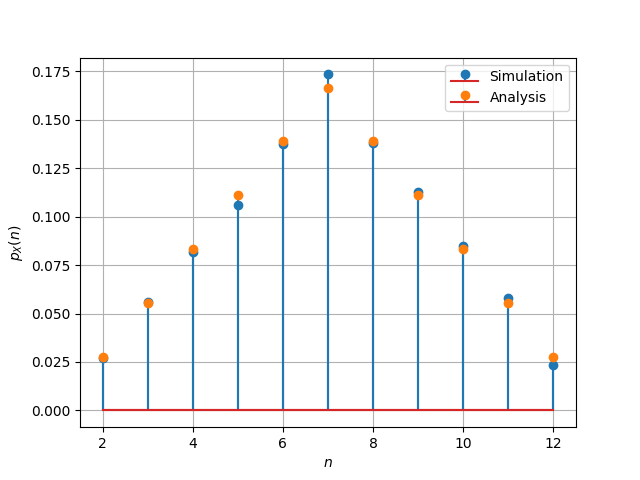
\includegraphics[width=\columnwidth]{./figs/sum/pmf.png}
\caption{Plot of $p_X(n)$.  Simulations are close to the analysis. }
\label{fig:dice}
\end{figure}
\item The python code is available in 
\begin{lstlisting}
/codes/sum/dice.py
\end{lstlisting}

%\item 
%We have shown how a simple problem of throwing a dice can be used for learning not just probability but concepts in  signal processing as well.  Inversion of the $Z$-transform for finding the pmf using contour integration, though not discussed here, opens a window to complex analysis too.  Note that the solutions that are provided  can be easily understood using high school math like arithmetic and geometric sums.  Thus, school students can use a bit of college level math to obtain simpler solutions to their problems.  College students can be exposed to advanced mathematics through simple problems from high school texts.  In addition, both can learn how to verify theoretical results through computer simulations.

%\bibliographystyle{tMES}
%\bibliography{school}
%
%\end{document}
\end{enumerate}

\section{Cumulative Distribution Function}
\subsection{The Bernoulli Distribution}
\renewcommand{\theequation}{\theenumi}
\begin{enumerate}[label=\thesection.\arabic*.,ref=\thesection.\theenumi]
\numberwithin{equation}{enumi}


\item A jar contains 24 marbles, some are green and others are blue. If a marble is drawn at random from the jar, the probability that it is green is $\frac{2}{3}$ Find the number of blue balls in the jar.
\item A bag contains lemon flavoured candies only. Malini takes out one candy without
looking into the bag. What is the probability that she takes out\\
(i) an orange flavoured candy?\\
(ii) a lemon flavoured candy?

\item 
\item 
\item 
\item 

\item It is known that 10$\%$ of certain articles manufactured are defective. What is the probability that in a random sample of 12 such articles, 9 are defective?\\
\item A person buys a lottery ticket in 50 lotteries, in each of which his chance of
winning a prize is $\frac{1}{100}$.What is the probability that he will win a prize\\
(a) at least once \\
(b) exactly once \\
(c) at least twice?\\
From the given information, the random variable representing the trials is
\begin{align}
X \sim B\brak{50,\frac{1}{100}}
\end{align}
%
Hence the desired probabilites are
\begin{enumerate}
\item 
\begin{align}
\pr{X \ge 1} = 1 - \pr{X =0} = 1-\brak{\frac{99}{100}}^{50} 
\end{align}
%
\item 
\begin{align}
\pr{X = 1} = {50}\brak{\frac{99}{100}}^{49} \brak{\frac{1}{100}}
\end{align}
%
\item 
\begin{align}
\pr{X \ge 2} &= 1 - \pr{X \le 1} 
\\
&= 1 - \pr{X =0} - \pr{X = 1} \\
&= 1 -\brak{\frac{149}{100}}\brak{\frac{99}{100}}^{49}\\
&= 0.0894
\end{align}

\end{enumerate}


\item In an examination, 20 questions of true-false type are asked. Suppose a student tosses a fair coin to determine his answer to each question. If the coin falls heads, he answers 'true'; if it falls tails, he answers 'false'. Find the probability that he answers at least 12 questions correctly.\\
\solution
Let $X_i \in \cbrak{0,1}$ represent the answer to the $i$th question.  From the given information,
\begin{align}
\pr{X=1} = p = \frac{1}{2}
\\
\pr{X=0} = q = 1-p
\end{align}
%
Defining 
\begin{align}
Y = \sum_{i=1}^{n}X_i,
\end{align}
the desire probability is
\begin{align}
\pr{Y \ge 12} &= \sum_{i=12}{20} \comb{20}{i}p^i q^{(20-i)} 
\\
&= 0.251722
\end{align}
$\because Y$  is a Bernoulli distribution with parameters $\brak{20,\frac{1}{2}}$.


\item There are 5$\%$ defective items in a large bulk of items. What is the probability
that a sample of 10 items will include not more than one defective item?\\
\solution
Let X be the random variable representing all the items.  Then,
\begin{align}
X = \sum_{i=1}^{10}X_i
\end{align}
%
has a Binomial distribution with
$X_i \in \cbrak{0,1}$ being a Bernoulli r.v. representing the item condition.  From the given information, the probability of an item being
defective is given by
\begin{align}
\pr{X_i = 0} &= \frac{1}{20} = p
\\
\implies \pr{X_i = 1} &= q = 1-p =  1-\frac{1}{20} = \frac{19}{20}
\end{align}
%
$\because$
 \begin{align}
    X &\sim B(n=10,p=0.5),
    \\
   \pr{X=r}&=    \comb{n}{r} p^r q^{n-r}
   \end{align}
\begin{multline}
\implies Pr(X \le 1)=Pr(X=0)+Pr(X=1) \\
              =\comb{10}{0}\left(\frac{1}{20}\right)^0 \left(\frac{19}{20}\right)^{10}+\comb{10}{1} \left(\frac{1}{20}\right)^1 \left(\frac{19}{20}\right)^{9}\\
              =\left(\frac{29}{20}\right) \times\left (\frac{19}{20}\right) ^{9}
              =0.9138
\end{multline} 



\item In a meeting, 70$\%$ of the members favour and 30$\%$ oppose a certain proposal.
A member is selected at random and we take X = 0 if he opposed, and X = 1 if he is in favour. Find E(X) and Var (X).\\
\solution
From the given information,
\begin{align}
\pr{X=0} = 70 {\%} = 0.7\\
\pr{X=1} = 30 {\%} =0.3
\end{align}
Hence,
\begin{align}
    E(X) &= 1\times0.7 + 0\times0.3 =0.7
    \\
    E(X^2) &= 1^2\times0.7 + 0^2\times0.3 =0.7
    \\
    \implies Var(X) &= E(X^2) -[E(X)]^2
    \\&= 0.7- 0.7^2 = 0.21
\end{align}

\item A coin is biased so that the head is 3 times as likely to occur as tail. If the coin is tossed twice, find the probability distribution of number of tails.\\
\item From a lot of 30 bulbs which include 6 defectives, a sample of 4 bulbs is drawn at random with replacement. Find the probability distribution of the number of defective bulbs.\\
\item Probability that A speaks truth is $\frac{4}{5}$. A coin is tossed. A reports that a head appears. The probability that actually there was head is\\
\begin{enumerate}
\item $\frac{4}{5}$
\item $\frac{1}{2}$
\item $\frac{1}{5}$
\item $\frac{2}{5}$
\end{enumerate}
\item A box of oranges is inspected by examining three randomly selected oranges drawn without replacement. If all the three oranges are good, the box is approved for sale, otherwise, it is rejected. Find the probability that a box containing 15 oranges out of which 12 are good and 3 are bad ones will be approved for sale.\\
\solution
%
Let the $i$th inspection be $X_i \in \cbrak{0,1}$, where  1 represents a good orange.  From the given information,
\begin{align}
\pr{X_1=1}&=\brak{\frac{12}{15}}\\ 
\pr{X_2=1|X_1=1}&=\brak{\frac{11}{14}} \\ 
\pr{X_3=1|X_1=1,X_2=1} &= \brak{\frac{10}{13}}
\end{align}
%
The probability that the box will be approved for sale is
\begin{multline}
\pr{X_1=1,X_2=1,X_3=1} 
\\
= \pr{X_1=1} \times \pr{X_2=1|X_1=1} 
\\
\times \pr{X_3=1|X_1=1,X_2=1} \\ 
=\frac{12}{15}\times \frac{11}{14} \times \frac{10}{13}\\ 
=\frac{1320}{2730} =0.483 
\end{multline}
%
\item Determine P(E/F), if a coin is tossed three times\\
(i) E : head on third toss , F : heads on first two tosses\\
(ii) E : at least two heads , F : at most two heads\\
(iii) E : at most two tails , F : at least one tail\\
%
\solution


\item Determine P(E/F), if two coins are tossed once, where\\
(i) E : tail appears on one coin, F : one coin shows head\\
(ii) E : no tail appears, F : no head appears\\
\item Two players, Sangeeta and Reshma, play a tennis match. It is known
that the probability of Sangeeta winning the match is 0.62. What is the probability of
Reshma winning the match?
\item Harpreet tosses two different coins simultaneously (say, one is of rupee 1
and other of rupee 2). What is the probability that she gets at least one head?

	\item In a cricket match, a batswoman hits a boundary 6 times out of 30 balls she plays. Find the probability that she did not hit a boundary.
\\
\solution
Let X be the random variable representing the number of defective eggs from the ten eggs picked. X follows a  binomial distribution.  Since the probability of an egg being defective is 10\%, substituting n=10, p= 0.1 and k=0 in equation \eqref{eq:exam41_1}, 
probability that there is atleast one defective egg is 
\begin{align}
\pr{X \geq 1}&= 1 - \pr{X=0}  = 1-\brak{0.9}^{10}
\\
&=0.6513215599
\end{align}
The python code for the above problem is,
\begin{lstlisting}
.solutions/20-10/prob/codes/exam42.py
\end{lstlisting}

	\item A coin is tossed 1000 times with the following frequencies:\\
Head : 455, Tail : 545\\
Compute the probability for each event.\\
\solution
\renewcommand{\theequation}{\theenumi}
\begin{enumerate}[label=\arabic*.,ref=\thesubsubsection.\theenumi]
\numberwithin{equation}{enumi}
\item In the given question,
\\
The sample size = Total number of possibilities(S)=6
\begin{align}
\myvec{1&2&3&4&5&6}
\end{align}
Event size= Odd number =3
\begin{align}
\myvec{1&3&5}
\end{align}
Probability for this event is = $\frac{1}{2}$
\\
The python code for the distribution of data,
\begin{lstlisting}
prob/codes/prob6_b.py
\end{lstlisting}
This shows the diagrametic representation of dice with the live update of probability with the role of dice.
\end{enumerate}

   \item Two coins are tossed simultaneously 500 times, and we get\\
       Two heads : 105 times\\
       One head : 275 times\\
       No head : 120 times\\
Find the probability of occurrence of each of these events.\\
\solution
Let $X_1\cbrak{0,1}$ represent the first coin and $X_2\cbrak{0,1}$ represent the second coin, where 0 represents tail and 1 represents head.  Define 
\begin{align}
X = X_1 + X_2,
\end{align}
Hence $X \in \cbrak{0,1,2}$.  From the given information, 
\begin{align}
\pr{X=1} &= \frac{105}{500}
\\
&= 0.21
\\
\pr{X=2} &= \frac{275}{500}
\\
&= 0.55
\\
\pr{X=0} &= \frac{120}{500}
\\
&= 0.24
\end{align}

   \item A die is thrown 1000 times with the frequencies for the outcomes 1, 2, 3, 4, 5 and 6 as given in the following Table \ref{table:prob_exam_3}.
Find the probability of getting each outcome.

\begin{table}[!ht]
\centering
\resizebox{\columnwidth}{!}{
\begin{tabular}{ |c|c|c|c|c|c|c| } 
 \hline
 \textbf{Outcome} &1 &2 &3 &4 &5 &6  \\ 
 \hline
 \textbf{Frequency} &179 &150 &157 &149 &175 &190 \\ 
 \hline
\end{tabular}
}
\caption{}
\label{table:prob_exam_3}
\end{table}
%\\
\solution
Let $X \in \cbrak{i}_{i=1}^{6}$ and $f_i$ be the correspnding frequency.  Then, 
\begin{align}
\pr{X=i} &= \frac{f_i}{1000}
\end{align}
The following code computes the probabilities
\begin{lstlisting}
solutions/1-10/codes/probexm/probexm3.py
\end{lstlisting}
%\begin{figure}[!ht]
%	\centering
%	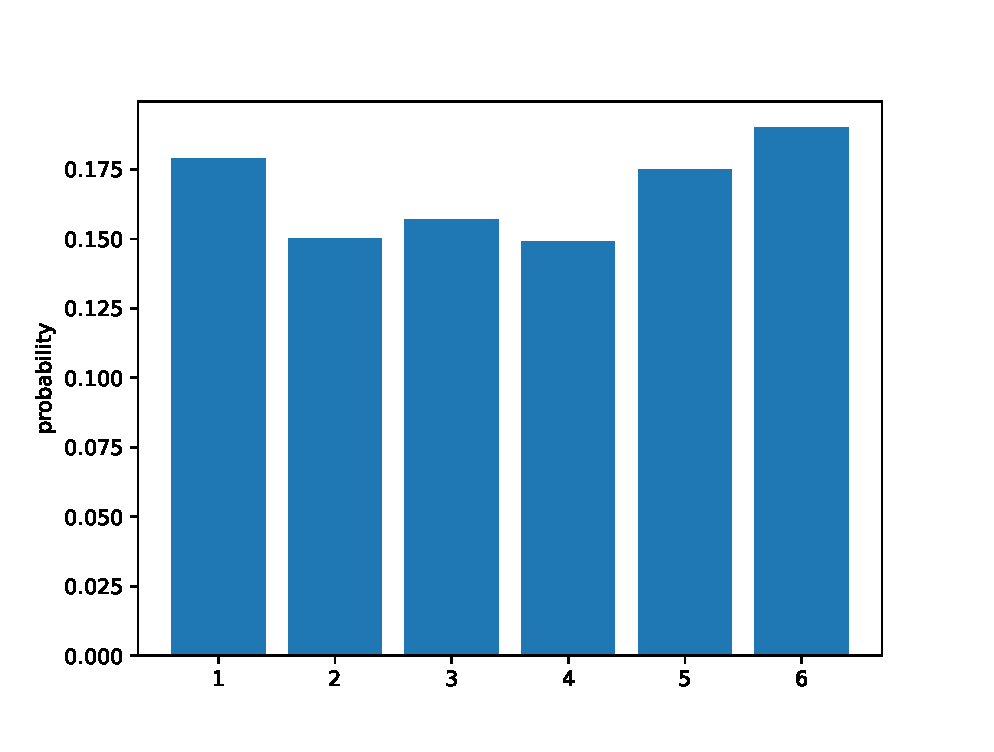
\includegraphics[width=\columnwidth]{./figures/probexm/probexm3.eps}
%	\caption{probability of outcome of biased dice }
%	\label{fig:bts3}
%	\begin{lstlisting}
%	figs/probexm/probexm3.eps
%	\end{lstlisting}
%\end{figure}


   \item The record of a weather station shows that out of the past 250 consecutive days, its weather forecasts were correct 175 times.\\
   (i) What is the probability that on a given day it was correct?\\
(ii) What is the probability that it was not correct on a given day?\\
\solution
Let $X \in \cbrak{0,1}$ be the random variable with 1 denoting correct forecast.
From the given information,
\begin{align}
\pr{X=1} & = \frac{175}{250}
\\
&= 0.7
\\
\pr{X=0} & = 1 - \pr{X=1}
\\
&= 0.3
\end{align}



\item {\em: Random Process}A and B throw a die alternatively till one of them gets a '6' and wins the game. Find their respective probabilities of winning, if A starts first.
\\
\solution
Let X be the random variable representing the number of defective eggs from the ten eggs picked. X follows a  binomial distribution.  Since the probability of an egg being defective is 10\%, substituting n=10, p= 0.1 and k=0 in equation \eqref{eq:exam41_1}, 
probability that there is atleast one defective egg is 
\begin{align}
\pr{X \geq 1}&= 1 - \pr{X=0}  = 1-\brak{0.9}^{10}
\\
&=0.6513215599
\end{align}
The python code for the above problem is,
\begin{lstlisting}
.solutions/20-10/prob/codes/exam42.py
\end{lstlisting}

%
\item To know the opinion of the students about the subject statistics, a survey of 200 students was conducted. The data is recorded in Table \ref{table:1.2.6}
Find the probability that a student chosen at random
\begin{enumerate}
\item likes statistics,
\item  does not like it.
\end{enumerate}
\begin{table}[!ht]
\centering
\begin{tabular}{ |c|c| } 
 \hline
 \textbf{Opinion} &\textbf{Number of students}\\
 \hline
 like  &135\\ 
 \hline
 dislike  &65\\ 
 \hline
\end{tabular}
\caption{}
\label{table:1.2.6}
\end{table}
\solution
Let X be the random variable representing the number of defective eggs from the ten eggs picked. X follows a  binomial distribution.  Since the probability of an egg being defective is 10\%, substituting n=10, p= 0.1 and k=0 in equation \eqref{eq:exam41_1}, 
probability that there is atleast one defective egg is 
\begin{align}
\pr{X \geq 1}&= 1 - \pr{X=0}  = 1-\brak{0.9}^{10}
\\
&=0.6513215599
\end{align}
The python code for the above problem is,
\begin{lstlisting}
.solutions/20-10/prob/codes/exam42.py
\end{lstlisting}

\item  Assume that each born child is equally likely to be a boy or a girl. If a family has two children, what is the conditional probability that both are girls given that\\
(i) the youngest is a girl,\\ 
(ii) at least one is a girl?\\
\solution

	\begin{table}[ht]
    \begin{center}
    	%%%%%%%%%%%%%%%%%%%%%%%%%%%%%%%%%%%%%%%%%%%%%%%%%%%%%%%%%%%%%%%%%%%%%%
%%                                                                  %%
%%  This is the header of a LaTeX2e file exported from Gnumeric.    %%
%%                                                                  %%
%%  This file can be compiled as it stands or included in another   %%
%%  LaTeX document. The table is based on the longtable package so  %%
%%  the longtable options (headers, footers...) can be set in the   %%
%%  preamble section below (see PRAMBLE).                           %%
%%                                                                  %%
%%  To include the file in another, the following two lines must be %%
%%  in the including file:                                          %%
%%        \def\inputGnumericTable{}                                 %%
%%  at the beginning of the file and:                               %%
%%        \input{name-of-this-file.tex}                             %%
%%  where the table is to be placed. Note also that the including   %%
%%  file must use the following packages for the table to be        %%
%%  rendered correctly:                                             %%
%%    \usepackage[latin1]{inputenc}                                 %%
%%    \usepackage{color}                                            %%
%%    \usepackage{array}                                            %%
%%    \usepackage{longtable}                                        %%
%%    \usepackage{calc}                                             %%
%%    \usepackage{multirow}                                         %%
%%    \usepackage{hhline}                                           %%
%%    \usepackage{ifthen}                                           %%
%%  optionally (for landscape tables embedded in another document): %%
%%    \usepackage{lscape}                                           %%
%%                                                                  %%
%%%%%%%%%%%%%%%%%%%%%%%%%%%%%%%%%%%%%%%%%%%%%%%%%%%%%%%%%%%%%%%%%%%%%%



%%  This section checks if we are begin input into another file or  %%
%%  the file will be compiled alone. First use a macro taken from   %%
%%  the TeXbook ex 7.7 (suggestion of Han-Wen Nienhuys).            %%
\def\ifundefined#1{\expandafter\ifx\csname#1\endcsname\relax}


%%  Check for the \def token for inputed files. If it is not        %%
%%  defined, the file will be processed as a standalone and the     %%
%%  preamble will be used.                                          %%
\ifundefined{inputGnumericTable}

%%  We must be able to close or not the document at the end.        %%
	\def\gnumericTableEnd{\end{document}}


%%%%%%%%%%%%%%%%%%%%%%%%%%%%%%%%%%%%%%%%%%%%%%%%%%%%%%%%%%%%%%%%%%%%%%
%%                                                                  %%
%%  This is the PREAMBLE. Change these values to get the right      %%
%%  paper size and other niceties.                                  %%
%%                                                                  %%
%%%%%%%%%%%%%%%%%%%%%%%%%%%%%%%%%%%%%%%%%%%%%%%%%%%%%%%%%%%%%%%%%%%%%%

	\documentclass[12pt%
			  %,landscape%
                    ]{report}
       \usepackage[latin1]{inputenc}
       \usepackage{fullpage}
       \usepackage{color}
       \usepackage{array}
       \usepackage{longtable}
       \usepackage{calc}
       \usepackage{multirow}
       \usepackage{hhline}
       \usepackage{ifthen}

	\begin{document}


%%  End of the preamble for the standalone. The next section is for %%
%%  documents which are included into other LaTeX2e files.          %%
\else

%%  We are not a stand alone document. For a regular table, we will %%
%%  have no preamble and only define the closing to mean nothing.   %%
    \def\gnumericTableEnd{}

%%  If we want landscape mode in an embedded document, comment out  %%
%%  the line above and uncomment the two below. The table will      %%
%%  begin on a new page and run in landscape mode.                  %%
%       \def\gnumericTableEnd{\end{landscape}}
%       \begin{landscape}


%%  End of the else clause for this file being \input.              %%
\fi

%%%%%%%%%%%%%%%%%%%%%%%%%%%%%%%%%%%%%%%%%%%%%%%%%%%%%%%%%%%%%%%%%%%%%%
%%                                                                  %%
%%  The rest is the gnumeric table, except for the closing          %%
%%  statement. Changes below will alter the table's appearance.     %%
%%                                                                  %%
%%%%%%%%%%%%%%%%%%%%%%%%%%%%%%%%%%%%%%%%%%%%%%%%%%%%%%%%%%%%%%%%%%%%%%

\providecommand{\gnumericmathit}[1]{#1} 
%%  Uncomment the next line if you would like your numbers to be in %%
%%  italics if they are italizised in the gnumeric table.           %%
%\renewcommand{\gnumericmathit}[1]{\mathit{#1}}
\providecommand{\gnumericPB}[1]%
{\let\gnumericTemp=\\#1\let\\=\gnumericTemp\hspace{0pt}}
 \ifundefined{gnumericTableWidthDefined}
        \newlength{\gnumericTableWidth}
        \newlength{\gnumericTableWidthComplete}
        \newlength{\gnumericMultiRowLength}
        \global\def\gnumericTableWidthDefined{}
 \fi
%% The following setting protects this code from babel shorthands.  %%
 \ifthenelse{\isundefined{\languageshorthands}}{}{\languageshorthands{english}}
%%  The default table format retains the relative column widths of  %%
%%  gnumeric. They can easily be changed to c, r or l. In that case %%
%%  you may want to comment out the next line and uncomment the one %%
%%  thereafter                                                      %%
\providecommand\gnumbox{\makebox[0pt]}
%%\providecommand\gnumbox[1][]{\makebox}

%% to adjust positions in multirow situations                       %%
\setlength{\bigstrutjot}{\jot}
\setlength{\extrarowheight}{\doublerulesep}

%%  The \setlongtables command keeps column widths the same across  %%
%%  pages. Simply comment out next line for varying column widths.  %%
\setlongtables

\setlength\gnumericTableWidth{%
	53pt+%
	53pt+%
	53pt+%
0pt}
\def\gumericNumCols{3}
\setlength\gnumericTableWidthComplete{\gnumericTableWidth+%
         \tabcolsep*\gumericNumCols*2+\arrayrulewidth*\gumericNumCols}
\ifthenelse{\lengthtest{\gnumericTableWidthComplete > \linewidth}}%
         {\def\gnumericScale{\ratio{\linewidth-%
                        \tabcolsep*\gumericNumCols*2-%
                        \arrayrulewidth*\gumericNumCols}%
{\gnumericTableWidth}}}%
{\def\gnumericScale{1}}

%%%%%%%%%%%%%%%%%%%%%%%%%%%%%%%%%%%%%%%%%%%%%%%%%%%%%%%%%%%%%%%%%%%%%%
%%                                                                  %%
%% The following are the widths of the various columns. We are      %%
%% defining them here because then they are easier to change.       %%
%% Depending on the cell formats we may use them more than once.    %%
%%                                                                  %%
%%%%%%%%%%%%%%%%%%%%%%%%%%%%%%%%%%%%%%%%%%%%%%%%%%%%%%%%%%%%%%%%%%%%%%

\ifthenelse{\isundefined{\gnumericColA}}{\newlength{\gnumericColA}}{}\settowidth{\gnumericColA}{\begin{tabular}{@{}p{53pt*\gnumericScale}@{}}x\end{tabular}}
\ifthenelse{\isundefined{\gnumericColB}}{\newlength{\gnumericColB}}{}\settowidth{\gnumericColB}{\begin{tabular}{@{}p{53pt*\gnumericScale}@{}}x\end{tabular}}
\ifthenelse{\isundefined{\gnumericColC}}{\newlength{\gnumericColC}}{}\settowidth{\gnumericColC}{\begin{tabular}{@{}p{53pt*\gnumericScale}@{}}x\end{tabular}}

\begin{tabular}[c]{%
	b{\gnumericColA}%
	b{\gnumericColB}%
	b{\gnumericColC}%
	}

%%%%%%%%%%%%%%%%%%%%%%%%%%%%%%%%%%%%%%%%%%%%%%%%%%%%%%%%%%%%%%%%%%%%%%
%%  The longtable options. (Caption, headers... see Goosens, p.124) %%
%	\caption{The Table Caption.}             \\	%
% \hline	% Across the top of the table.
%%  The rest of these options are table rows which are placed on    %%
%%  the first, last or every page. Use \multicolumn if you want.    %%

%%  Header for the first page.                                      %%
%	\multicolumn{3}{c}{The First Header} \\ \hline 
%	\multicolumn{1}{c}{colTag}	%Column 1
%	&\multicolumn{1}{c}{colTag}	%Column 2
%	&\multicolumn{1}{c}{colTag}	\\ \hline %Last column
%	\endfirsthead

%%  The running header definition.                                  %%
%	\hline
%	\multicolumn{3}{l}{\ldots\small\slshape continued} \\ \hline
%	\multicolumn{1}{c}{colTag}	%Column 1
%	&\multicolumn{1}{c}{colTag}	%Column 2
%	&\multicolumn{1}{c}{colTag}	\\ \hline %Last column
%	\endhead

%%  The running footer definition.                                  %%
%	\hline
%	\multicolumn{3}{r}{\small\slshape continued\ldots} \\
%	\endfoot

%%  The ending footer definition.                                   %%
%	\multicolumn{3}{c}{That's all folks} \\ \hline 
%	\endlastfoot
%%%%%%%%%%%%%%%%%%%%%%%%%%%%%%%%%%%%%%%%%%%%%%%%%%%%%%%%%%%%%%%%%%%%%%

\hhline{|-|-~}
	 \multicolumn{1}{|p{\gnumericColA}|}%
	{\gnumericPB{\centering}\gnumbox{Mark}}
	&\multicolumn{1}{p{\gnumericColB}|}%
	{\gnumericPB{\centering}\gnumbox{Frequency}}
	&
\\
\hhline{|--|~}
	 \multicolumn{1}{|p{\gnumericColA}|}%
	{\gnumericPB{\centering}\gnumbox{2}}
	&\multicolumn{1}{p{\gnumericColB}|}%
	{\gnumericPB{\centering}\gnumbox{1}}
	&
\\
\hhline{|--|~}
	 \multicolumn{1}{|p{\gnumericColA}|}%
	{\gnumericPB{\centering}\gnumbox{3}}
	&\multicolumn{1}{p{\gnumericColB}|}%
	{\gnumericPB{\centering}\gnumbox{2}}
	&
\\
\hhline{|--|~}
	 \multicolumn{1}{|p{\gnumericColA}|}%
	{\gnumericPB{\centering}\gnumbox{4}}
	&\multicolumn{1}{p{\gnumericColB}|}%
	{\gnumericPB{\centering}\gnumbox{3}}
	&
\\
\hhline{|--|~}
	 \multicolumn{1}{|p{\gnumericColA}|}%
	{\gnumericPB{\centering}\gnumbox{5}}
	&\multicolumn{1}{p{\gnumericColB}|}%
	{\gnumericPB{\centering}\gnumbox{2}}
	&
\\
\hhline{|--|~}
	 \multicolumn{1}{|p{\gnumericColA}|}%
	{\gnumericPB{\centering}\gnumbox{6}}
	&\multicolumn{1}{p{\gnumericColB}|}%
	{\gnumericPB{\centering}\gnumbox{3}}
	&
\\
\hhline{|--|~}
	 \multicolumn{1}{|p{\gnumericColA}|}%
	{\gnumericPB{\centering}\gnumbox{7}}
	&\multicolumn{1}{p{\gnumericColB}|}%
	{\gnumericPB{\centering}\gnumbox{3}}
	&
\\
\hhline{|--|~}
	 \multicolumn{1}{|p{\gnumericColA}|}%
	{\gnumericPB{\centering}\gnumbox{9}}
	&\multicolumn{1}{p{\gnumericColB}|}%
	{\gnumericPB{\centering}\gnumbox{4}}
	&
\\
\hhline{|--|~}
	 \multicolumn{1}{|p{\gnumericColA}|}%
	{\gnumericPB{\centering}\gnumbox{10}}
	&\multicolumn{1}{p{\gnumericColB}|}%
	{\gnumericPB{\centering}\gnumbox{2}}
	&
\\
\hhline{|-|-|~}
\end{tabular}

\ifthenelse{\isundefined{\languageshorthands}}{}{\languageshorthands{\languagename}}
\gnumericTableEnd

  \caption{Marks obtained by students}
   \label{table:statsex_23table1}
   \end{center}	
\end{table}

As we can see from table \ref{table:statsex_23table1}, 9 occurs the maximum number of times.\\
Thus Mode = 9.




\item  An instructor has a question bank consisting of 300 easy True / False questions,
200 difficult True / False questions, 500 easy multiple choice questions and 400 difficult multiple choice questions. If a question is selected at random from the question bank, what is the probability that it will be an easy question given that it is a multiple choice question?\\
\solution
From the given information, using the fact that $A,B$ are independent,
\begin{align}
\pr{A+B} &= \pr{A}+\pr{B}-\pr{AB}
\\
&= \pr{A} + \pr{B-AB} 
\\
&= \pr{A} + \pr{A'B}
\\
&= \pr{A} + \pr{A'}\pr{B}
\\
&= \pr{A} + \pr{A'}\brak{1-\pr{B'}}
\\
&= \pr{A} + \pr{A'}-\pr{A'}\pr{B'}
\\
&=1 - \pr{A'}\pr{B'}
\end{align}


\item Two cards are drawn at random and without replacement from a pack of 52 playing cards. Find the probability that both the cards are black.\\
\solution
Let $X_1,X_2 \in \cbrak{0,1}$ represent the colour, where 0 denotes black and 1 denotes red.  From the given information,
\begin{align}
\pr{X_1 = 0} &= \frac{26}{52}= \frac{1}{2}
\\
\pr{X_2 = 0|X_1 = 0} &= \frac{25}{51}
\end{align}
Then,
\begin{multline}
\pr{X_1=0,X_2=0} 
\\
= \pr{X_2 = 0|X_1 = 0}\pr{X_1 = 0}
 = \frac{25}{102}
\end{multline}

\item Two balls are drawn at random with replacement from a box containing 10 black and 8 red balls. Find the probability that\\
(i) both balls are red.\\
(ii) first ball is black and second is red.\\
(iii) one of them is black and other is red.\\
\solution
Let X be the random variable representing the number of defective eggs from the ten eggs picked. X follows a  binomial distribution.  Since the probability of an egg being defective is 10\%, substituting n=10, p= 0.1 and k=0 in equation \eqref{eq:exam41_1}, 
probability that there is atleast one defective egg is 
\begin{align}
\pr{X \geq 1}&= 1 - \pr{X=0}  = 1-\brak{0.9}^{10}
\\
&=0.6513215599
\end{align}
The python code for the above problem is,
\begin{lstlisting}
.solutions/20-10/prob/codes/exam42.py
\end{lstlisting}


\item Probability of solving specific problem independently by A and B are $\frac{1}{2}$
and $\frac{1}{3}$ respectively. If both try to solve the problem independently, find the probability that\\
(i) the problem is solved \\
(ii) exactly one of them solves the problem.\\
\solution
Let X be the random variable representing the number of defective eggs from the ten eggs picked. X follows a  binomial distribution.  Since the probability of an egg being defective is 10\%, substituting n=10, p= 0.1 and k=0 in equation \eqref{eq:exam41_1}, 
probability that there is atleast one defective egg is 
\begin{align}
\pr{X \geq 1}&= 1 - \pr{X=0}  = 1-\brak{0.9}^{10}
\\
&=0.6513215599
\end{align}
The python code for the above problem is,
\begin{lstlisting}
.solutions/20-10/prob/codes/exam42.py
\end{lstlisting}

\item (i) A lot of 20 bulbs contain 4 defective ones. One bulb is drawn at random from the lot.
What is the probability that this bulb is defective?\\
(ii) Suppose the bulb drawn in (i) is not defective and is not replaced. Now one bulb
is drawn at random from the rest. What is the probability that this bulb is not
defective ?
\\
\solution
Let X be the random variable representing the number of defective eggs from the ten eggs picked. X follows a  binomial distribution.  Since the probability of an egg being defective is 10\%, substituting n=10, p= 0.1 and k=0 in equation \eqref{eq:exam41_1}, 
probability that there is atleast one defective egg is 
\begin{align}
\pr{X \geq 1}&= 1 - \pr{X=0}  = 1-\brak{0.9}^{10}
\\
&=0.6513215599
\end{align}
The python code for the above problem is,
\begin{lstlisting}
.solutions/20-10/prob/codes/exam42.py
\end{lstlisting}

\item 12 defective pens are accidentally mixed with 132 good ones. It is not possible to just
look at a pen and tell whether or not it is defective. One pen is taken out at random from
this lot. Determine the probability that the pen taken out is a good one.
\\
\solution
Let X be the random variable representing the number of defective eggs from the ten eggs picked. X follows a  binomial distribution.  Since the probability of an egg being defective is 10\%, substituting n=10, p= 0.1 and k=0 in equation \eqref{eq:exam41_1}, 
probability that there is atleast one defective egg is 
\begin{align}
\pr{X \geq 1}&= 1 - \pr{X=0}  = 1-\brak{0.9}^{10}
\\
&=0.6513215599
\end{align}
The python code for the above problem is,
\begin{lstlisting}
.solutions/20-10/prob/codes/exam42.py
\end{lstlisting}

\item Gopi buys a fish from a shop for his aquarium. The
shopkeeper takes out one fish at random from a
tank containing 5 male fish and 8 female fish (see
Fig. \ref{fig:prob_121}). What is the probability that the fish taken
out is a male fish?
\begin{figure}[!ht]
\centering
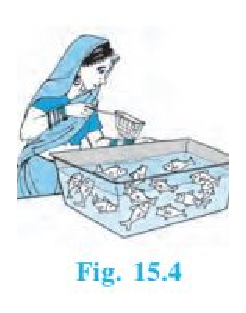
\includegraphics[width=\columnwidth]{./prob/figs/woman.eps}
\caption{}
\label{fig:prob_121}
\end{figure}
\\
\solution
Let X be the random variable representing the number of defective eggs from the ten eggs picked. X follows a  binomial distribution.  Since the probability of an egg being defective is 10\%, substituting n=10, p= 0.1 and k=0 in equation \eqref{eq:exam41_1}, 
probability that there is atleast one defective egg is 
\begin{align}
\pr{X \geq 1}&= 1 - \pr{X=0}  = 1-\brak{0.9}^{10}
\\
&=0.6513215599
\end{align}
The python code for the above problem is,
\begin{lstlisting}
.solutions/20-10/prob/codes/exam42.py
\end{lstlisting}
    
\item A lot consists of 144 ball pens of which 20 are defective and the others are good. Nuri will buy a pen if it is good, but will not buy if it is defective. The shopkeeper draws one pen at random and gives it to her. What is the probability that\\
(i) She will buy it ?\\
(ii) She will not buy it ?
\\
\solution
Let X be the random variable representing the number of defective eggs from the ten eggs picked. X follows a  binomial distribution.  Since the probability of an egg being defective is 10\%, substituting n=10, p= 0.1 and k=0 in equation \eqref{eq:exam41_1}, 
probability that there is atleast one defective egg is 
\begin{align}
\pr{X \geq 1}&= 1 - \pr{X=0}  = 1-\brak{0.9}^{10}
\\
&=0.6513215599
\end{align}
The python code for the above problem is,
\begin{lstlisting}
.solutions/20-10/prob/codes/exam42.py
\end{lstlisting}


\item A bag contains 5 red balls and some blue balls. If the probability of drawing a blue ball is double that of a red ball, determine the number of blue balls in the bag.
\\
\solution
Let X be the random variable representing the number of defective eggs from the ten eggs picked. X follows a  binomial distribution.  Since the probability of an egg being defective is 10\%, substituting n=10, p= 0.1 and k=0 in equation \eqref{eq:exam41_1}, 
probability that there is atleast one defective egg is 
\begin{align}
\pr{X \geq 1}&= 1 - \pr{X=0}  = 1-\brak{0.9}^{10}
\\
&=0.6513215599
\end{align}
The python code for the above problem is,
\begin{lstlisting}
.solutions/20-10/prob/codes/exam42.py
\end{lstlisting}

\item A box contains 12 balls out of which x are black. If one ball is drawn at random from the box,what is the probability that it will be a black ball?\\
If 6 more black balls are put in the box, the probability of drawing a black ball is now double of what it was before. Find x.
\\
\solution
Let X be the random variable representing the number of defective eggs from the ten eggs picked. X follows a  binomial distribution.  Since the probability of an egg being defective is 10\%, substituting n=10, p= 0.1 and k=0 in equation \eqref{eq:exam41_1}, 
probability that there is atleast one defective egg is 
\begin{align}
\pr{X \geq 1}&= 1 - \pr{X=0}  = 1-\brak{0.9}^{10}
\\
&=0.6513215599
\end{align}
The python code for the above problem is,
\begin{lstlisting}
.solutions/20-10/prob/codes/exam42.py
\end{lstlisting}

\end{enumerate}
%\end{document}
    

\subsection{The Binomial Distribution}
\renewcommand{\theequation}{\theenumi}
\begin{enumerate}[label=\arabic*.,ref=\thesubsection.\theenumi]
\numberwithin{equation}{enumi}


\item How many times must a man toss a fair coin so that the probability of having at least one head is more than 90$\%$?\\
\item An experiment succeeds twice as often as it fails. Find the probability that in the next six trials, there will be at least 4 successes.\\
\item Suppose X has a binomial distribution . Show that X = 3 is the most likely outcome.\\
(Hint : P(X = 3) is the maximum among all P($x_i$), $x_i$= 0,1,2,3,4,5,6)\\
\item The probability that a bulb produced by a factory will fuse after 150 days of use
is 0.05. Find the probability that out of 5 such bulbs\\
(i) none\\
(ii) not more than one\\
(iii) more than one\\
(iv) at least one\\
will fuse after 150 days of use.\\
\item Find the mean number of heads in three tosses of a fair coin.\\

\item Find the probability distribution of\\
(i) number of heads in two tosses of a coin.\\
(ii) number of tails in the simultaneous tosses of three coins.\\
(iii) number of heads in four tosses of a coin.\\
\item Let X represent the difference between the number of heads and the number of tails obtained when a coin is tossed 6 times. What are possible values of X?\\
\item Six balls are drawn successively from an urn containing 7 red and 9 black balls. Tell whether or not the trials of drawing balls are Bernoulli trials when after each draw the ball drawn is\\
(i) replaced \\
(ii) not replaced in the urn.\\

\item If a fair coin is tossed 10 times, find the probability of
\begin{enumerate}
\item  exactly six heads
\item  at least six heads
\item  at most six  heads
\end{enumerate}
\solution
Let X be the random variable representing the number of defective eggs from the ten eggs picked. X follows a  binomial distribution.  Since the probability of an egg being defective is 10\%, substituting n=10, p= 0.1 and k=0 in equation \eqref{eq:exam41_1}, 
probability that there is atleast one defective egg is 
\begin{align}
\pr{X \geq 1}&= 1 - \pr{X=0}  = 1-\brak{0.9}^{10}
\\
&=0.6513215599
\end{align}
The python code for the above problem is,
\begin{lstlisting}
.solutions/20-10/prob/codes/exam42.py
\end{lstlisting}


\item Ten eggs are drawn successively with replacement from a lot containing 10$\%$ defective eggs. Find the probability that there is at least one defective egg.\\
\solution
Let X be the random variable representing the number of defective eggs from the ten eggs picked. X follows a  binomial distribution.  Since the probability of an egg being defective is 10\%, substituting n=10, p= 0.1 and k=0 in equation \eqref{eq:exam41_1}, 
probability that there is atleast one defective egg is 
\begin{align}
\pr{X \geq 1}&= 1 - \pr{X=0}  = 1-\brak{0.9}^{10}
\\
&=0.6513215599
\end{align}
The python code for the above problem is,
\begin{lstlisting}
.solutions/20-10/prob/codes/exam42.py
\end{lstlisting}


\item Find the mean of the Binomial distribution B(4,$\frac{1}{3}$).
\\
\solution
Let X be the random variable representing the number of defective eggs from the ten eggs picked. X follows a  binomial distribution.  Since the probability of an egg being defective is 10\%, substituting n=10, p= 0.1 and k=0 in equation \eqref{eq:exam41_1}, 
probability that there is atleast one defective egg is 
\begin{align}
\pr{X \geq 1}&= 1 - \pr{X=0}  = 1-\brak{0.9}^{10}
\\
&=0.6513215599
\end{align}
The python code for the above problem is,
\begin{lstlisting}
.solutions/20-10/prob/codes/exam42.py
\end{lstlisting}


\item The probability of a shooter hitting a target is $\frac{3}{4}$. How many minimum
number of times must he/she fire so that the probability of hitting the target at least
once is more than 0.99?
\\
\solution
Let X be the random variable representing the number of defective eggs from the ten eggs picked. X follows a  binomial distribution.  Since the probability of an egg being defective is 10\%, substituting n=10, p= 0.1 and k=0 in equation \eqref{eq:exam41_1}, 
probability that there is atleast one defective egg is 
\begin{align}
\pr{X \geq 1}&= 1 - \pr{X=0}  = 1-\brak{0.9}^{10}
\\
&=0.6513215599
\end{align}
The python code for the above problem is,
\begin{lstlisting}
.solutions/20-10/prob/codes/exam42.py
\end{lstlisting}


\item Three coins are tossed simultaneously. Consider the event E "three heads or three tails", F "at least two heads" and G "at most two heads". Of the pairs (E,F), (E,G) and (F,G), which are independent? which are dependent?\\
\solution
Arranging the points scored by the  team in ascending order we get:\\
2,5,7,7,8,8,10,10,14,15,17,18,24,27,28,48\\
Let N be the no. of observations = 16\\
\begin{align}
\text{Median} = \frac{\brak{\frac{N}{2}}^{th}\text{value} + \brak{\frac{N}{2}+1}^{th}\text{value}}{2}
\end{align}

\begin{align}
\text{Median} &= \frac{\brak{8}^{th}\text{value} + \brak{9}^{th}\text{value}}{2}\\
\text{Median} &= \frac{10 + 14}{2}\\
\text{Median} &= 12
\end{align}

\item A die is tossed thrice. Find the probability of getting an odd number at least once.\\
\\
\solution
Let X be the random variable representing the number of defective eggs from the ten eggs picked. X follows a  binomial distribution.  Since the probability of an egg being defective is 10\%, substituting n=10, p= 0.1 and k=0 in equation \eqref{eq:exam41_1}, 
probability that there is atleast one defective egg is 
\begin{align}
\pr{X \geq 1}&= 1 - \pr{X=0}  = 1-\brak{0.9}^{10}
\\
&=0.6513215599
\end{align}
The python code for the above problem is,
\begin{lstlisting}
.solutions/20-10/prob/codes/exam42.py
\end{lstlisting}

\item A game consists of tossing a one rupee coin 3 times and noting its outcome each time. Hanif wins if all the tosses give the same result i.e., three heads or three tails, and loses otherwise. Calculate the probability that Hanif will lose the game.
\\
\solution
Let X be the random variable representing the number of defective eggs from the ten eggs picked. X follows a  binomial distribution.  Since the probability of an egg being defective is 10\%, substituting n=10, p= 0.1 and k=0 in equation \eqref{eq:exam41_1}, 
probability that there is atleast one defective egg is 
\begin{align}
\pr{X \geq 1}&= 1 - \pr{X=0}  = 1-\brak{0.9}^{10}
\\
&=0.6513215599
\end{align}
The python code for the above problem is,
\begin{lstlisting}
.solutions/20-10/prob/codes/exam42.py
\end{lstlisting}

\item A die is thrown twice. What is the probability that\\
\begin{enumerate}[label=(\roman*)]
\item  5 will not come up either time? \\
\item  5 will come up at least once?\\
\end{enumerate}
Hint : Throwing a die twice and throwing two dice simultaneously are treated as the
same experiment
\\
\solution
Let X be the random variable representing the number of defective eggs from the ten eggs picked. X follows a  binomial distribution.  Since the probability of an egg being defective is 10\%, substituting n=10, p= 0.1 and k=0 in equation \eqref{eq:exam41_1}, 
probability that there is atleast one defective egg is 
\begin{align}
\pr{X \geq 1}&= 1 - \pr{X=0}  = 1-\brak{0.9}^{10}
\\
&=0.6513215599
\end{align}
The python code for the above problem is,
\begin{lstlisting}
.solutions/20-10/prob/codes/exam42.py
\end{lstlisting}


\end{enumerate}



\section{Central Limit Theorem: Gaussian Distribution}
\renewcommand{\thefigure}{\theenumi}
\renewcommand{\thetable}{\theenumi}
%%
%\begin{enumerate}[label=\thesection.\arabic*
%,ref=\thesection.\theenumi]

\subsection{Bernoulli to Gaussian}
\begin{enumerate}[label=\thesubsection.\arabic*
,ref=\thesection.\theenumi]


\item {\em Mean :}  The mean of the bernoulli distribution is 
\begin{align}
\mu = E\brak{X_i}  = \sum_{k=0}^{1}kp_{X_i}(k) = p = \frac{1}{6}
\end{align}
\item {\em Moment:}  The moment of the distribution is defined as
\begin{align}
E\brak{X_i^r}  = \sum_{k=0}^{1}k^rp_{X_i}(k) = p = \frac{1}{6}
\end{align}

%The second moment of the bernoulli distribution is 
%\begin{align}
%E\brak{X_i}  = \sum_{k=0}^{1}kp_{X_i}(k) = p = \frac{1}{6}
%\end{align}
\item {\em Variance :}  The variance of the bernoulli distribution is defined as
\begin{align}
\sigma^2 &= E\brak{X-E\brak{X}}^2  = E\brak{X^2}-E^2\brak{X} 
\\
&=p-p^2 = p\brak{1-p} = \frac{5}{36}
\end{align}
%
The standard deviation 
\begin{align}
\sigma =  \sqrt{p\brak{1-p}}
\end{align}
%
\item {\em The Gaussian Distribution: }  Define
\begin{align}
\label{eq:bern_gauss}
G = \frac{1}{\sqrt{n}}\sum_{k=1}^{n}\frac{X_i-\mu}{\sigma}
\end{align}
%
\item {\em Approximating Binomial Using Gaussian: } From \eqref{eq:bern_gauss}
and \eqref{eq:bern_binom},
%
\begin{align}
X & \approx \sigma\sqrt{n}G + n\mu 
\\
\implies F_X(k) &= \pr{\sigma\sqrt{n}G + n\mu  \le k }
\\
 &= F_G\brak{\frac{k-n\mu}{\sigma\sqrt{n}}} \approx \phi\brak{\frac{k-n\mu}{\sigma\sqrt{n}}} 
\label{eq:bern_gaussian_cdf}
\end{align}
where 
\begin{align}
\phi_{X}(x) = \int^{x}_{-\infty} \frac{1}{\sqrt{2\pi}}e^{-\frac{x^2}{2}}, -\infty < x < \infty
\end{align}
\item The 
probability density function (PDF) 
of $G$ is
%
\begin{align}
p_{G}(x) &= \frac{d}{dx}F_{X}(x)
\\
 &=  \frac{1}{{\sigma\sqrt{n}}}\phi^{\prime}\brak{\frac{k-n\mu}{\sigma\sqrt{n}}} 
\label{eq:bern_gaussian_pdf}
\end{align}
%
For large $n$, $G$ is a continuous distribution with probability density function (PDF)
\begin{align}
p_G(x) =  \frac{1}{\sqrt{2\pi}}\exp\brak{-\frac{x^2}{2}}, -\infty < x < \infty,
\end{align}
%
\item {\em Evaluationg the Probability: }  From \ref{eq:bern_gaussian_cdf}
and \ref{eq:bern_gaussian_pdf},
\begin{align}
\pr{X \le 1 } &= F_{G}(1) = p_G(0)+p_G(1) 
\\
&\approx 
0.41299463887797094
\label{eq:bern_gauss_ans}
\end{align}
which is close to \eqref{eq:bern_binom_ans}.
%
\end{enumerate}
\subsection{Uniform to Gaussian}
\begin{enumerate}[label=\thesubsection.\arabic*
,ref=\thesection.\theenumi]

\item
Generate $10^6$ samples of the random variable
%
\begin{equation}
X = \sum_{i=1}^{12}U_i -6
\end{equation}
%
using a C program, where $U_i, i = 1,2,\dots, 12$ are  a set of independent uniform random variables between 0 and 1
and save in a file called gau.dat
\\
\solution Download the following files and execute the  C program.
\begin{lstlisting}
codes/cdf/exrand.c
codes/cdf/coeffs.h
\end{lstlisting}

%
\item
Load gau.dat in python and plot the empirical CDF of $X$ using the samples in gau.dat. What properties does a CDF have?
\\
\solution The CDF of $X$ is plotted in Fig. \ref{fig:gauss_cdf}
\begin{figure}
\centering
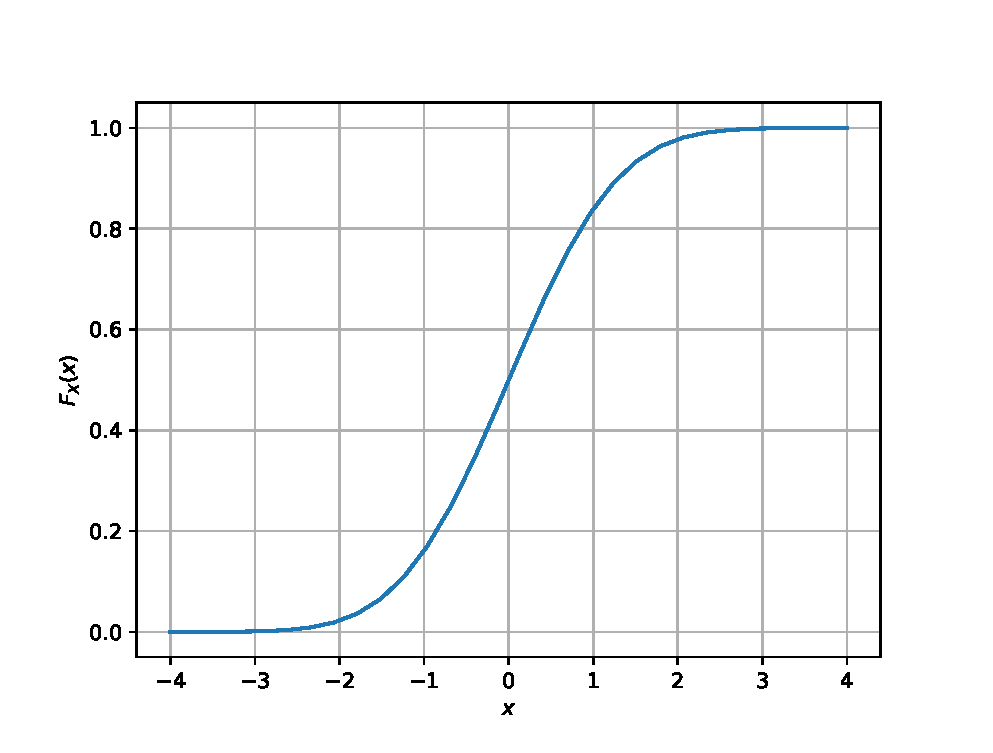
\includegraphics[width=\columnwidth]{./figs/clt/gauss_cdf}
\caption{The CDF of $X$}
\label{fig:gauss_cdf}
\end{figure}


\item
Load gau.dat in python and plot the empirical PDF of $X$ using the samples in gau.dat. The PDF of $X$ is defined as
\begin{align}
p_{X}(x) = \frac{d}{dx}F_{X}(x)
\end{align}
What properties does the PDF have?
\\
\solution The PDF of $X$ is plotted in Fig. \ref{fig:gauss_pdf} using the code below
\begin{lstlisting}
codes/clt/pdf_plot.py
\end{lstlisting}

\begin{figure}
\centering
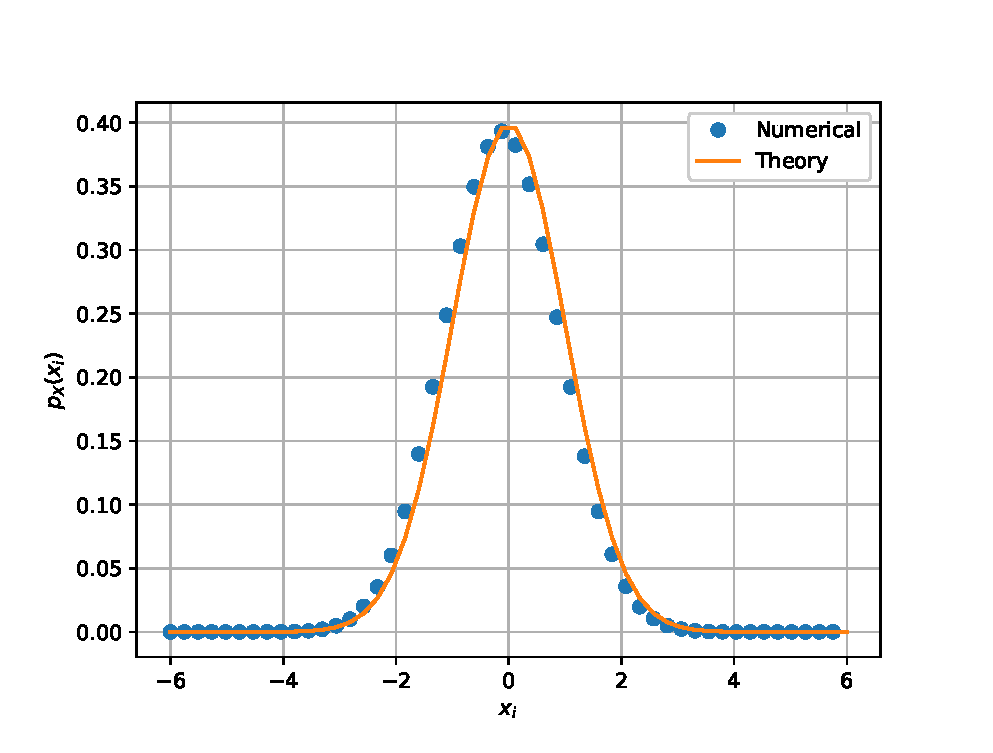
\includegraphics[width=\columnwidth]{./figs/clt/gauss_pdf}
\caption{The PDF of $X$}
\label{fig:gauss_pdf}
\end{figure}

\item Find the mean and variance of $X$ by writing a C program.
\\
\solution  Execute
\begin{lstlisting}
codes/clt/gaussian_numbers.c
\end{lstlisting}
\item Given that 
\begin{align}
p_{X}(x) = \frac{1}{\sqrt{2\pi}}\exp\brak{-\frac{x^2}{2}}, -\infty < x < \infty,
\end{align}
repeat the above exercise theoretically.
%
\\
\solution
Let X be the random variable representing the number of defective eggs from the ten eggs picked. X follows a  binomial distribution.  Since the probability of an egg being defective is 10\%, substituting n=10, p= 0.1 and k=0 in equation \eqref{eq:exam41_1}, 
probability that there is atleast one defective egg is 
\begin{align}
\pr{X \geq 1}&= 1 - \pr{X=0}  = 1-\brak{0.9}^{10}
\\
&=0.6513215599
\end{align}
The python code for the above problem is,
\begin{lstlisting}
.solutions/20-10/prob/codes/exam42.py
\end{lstlisting}

\item Let $U$ be a uniform random variable between 0 and 1.
%\begin{enumerate}[label=\thesection.\arabic*
%,ref=\thesection.\theenumi]

%
\item
Load the uni.dat file into python and plot the empirical CDF of $U$ using the samples in uni.dat. The CDF is defined as
\begin{align}
F_{U}(x) = \pr{U \le x}
\end{align}
\\
\solution  The following code plots Fig. \ref{fig:uni_cdf}
\begin{lstlisting}
codes/cdf/cdf_plot.py
\end{lstlisting}
\begin{figure}
\centering
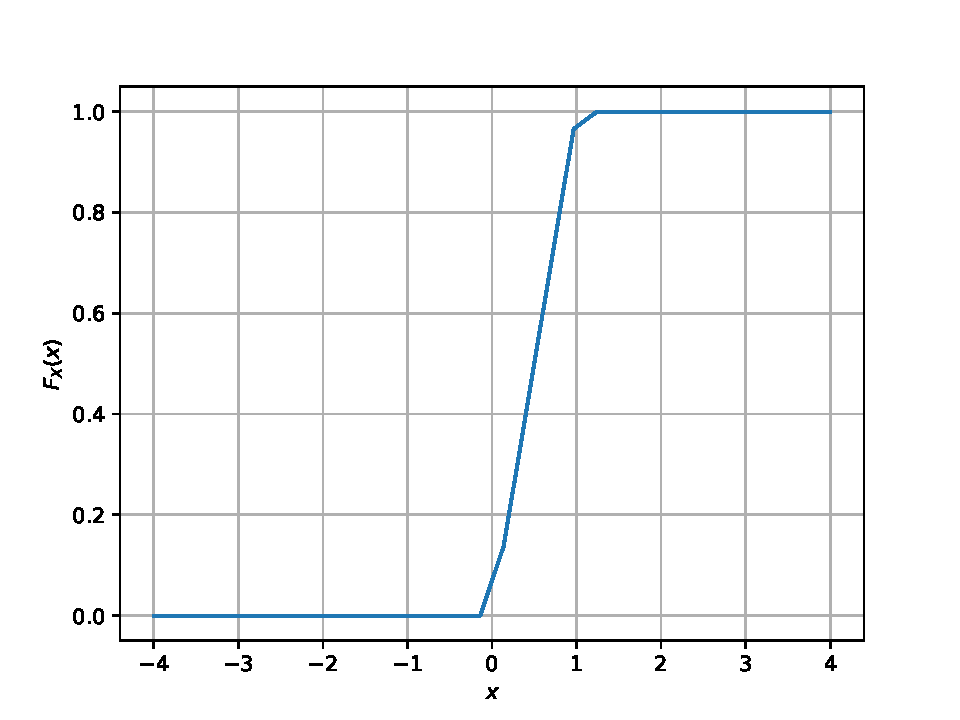
\includegraphics[width=\columnwidth]{./figs/cdf/uni_cdf}
\caption{The CDF of $U$}
\label{fig:uni_cdf}
\end{figure}

%\item Generate $10^6$ samples of $U$ using a C program and save into a file called uni.dat .
%\\


%
\item
Find a  theoretical expression for $F_{U}(x)$.

\item
The mean of $U$ is defined as
%
\begin{equation}
E\sbrak{U} = \frac{1}{N}\sum_{i=1}^{N}U_i
\end{equation}
%
and its variance as
%
\begin{equation}
\text{var}\sbrak{U} = E\sbrak{U- E\sbrak{U}}^2 
\end{equation}

Write a C program to  find the mean and variance of $U$. 
\item Verify your result theoretically given that
%
\begin{equation}
E\sbrak{U^k} = \int_{-\infty}^{\infty}x^kdF_{U}(x)
\end{equation}

\end{enumerate}




%\section{Cumulative Distribution Function}
%\renewcommand{\thefigure}{\theenumi}
\renewcommand{\thetable}{\theenumi}
%%
Let $U$ be a uniform random variable between 0 and 1.
%\begin{enumerate}[label=\thesection.\arabic*
%,ref=\thesection.\theenumi]
\item Generate $10^6$ samples of $U$ using a C program and save into a file called uni.dat .
\\
\solution Download the following files and execute the  C program.
\begin{lstlisting}
codes/cdf/exrand.c
codes/cdf/coeffs.h
\end{lstlisting}

%
\item
Load the uni.dat file into python and plot the empirical CDF of $U$ using the samples in uni.dat. The CDF is defined as
\begin{align}
F_{U}(x) = \pr{U \le x}
\end{align}
\\
\solution  The following code plots Fig. \ref{fig:uni_cdf}
\begin{lstlisting}
codes/cdf/cdf_plot.py
\end{lstlisting}
\begin{figure}
\centering
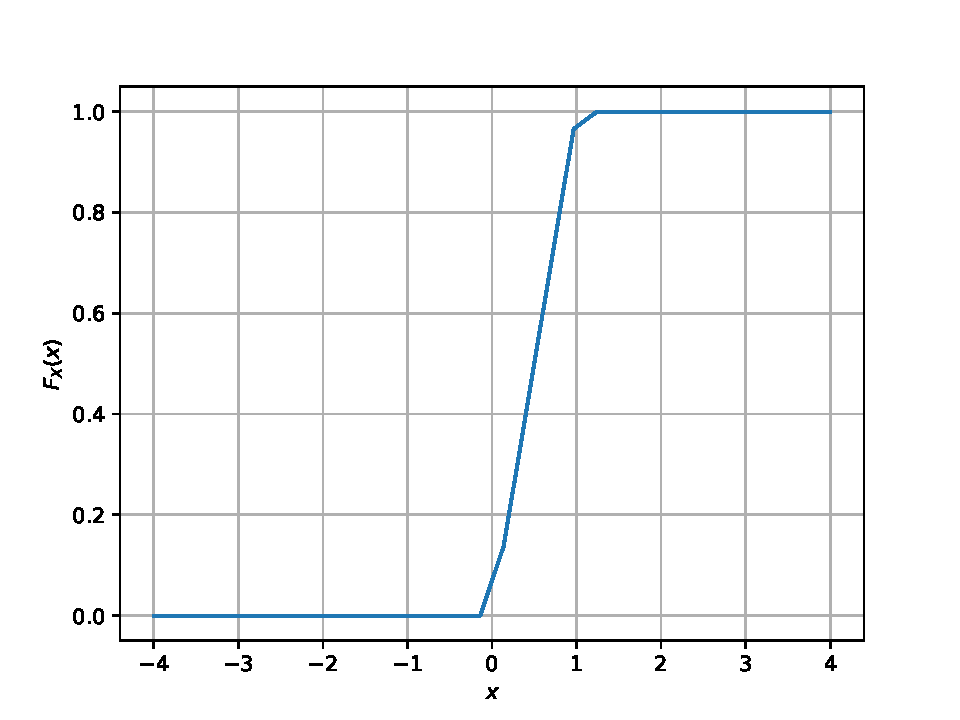
\includegraphics[width=\columnwidth]{./figs/cdf/uni_cdf}
\caption{The CDF of $U$}
\label{fig:uni_cdf}
\end{figure}

%
\item
Find a  theoretical expression for $F_{U}(x)$.

\item
The mean of $U$ is defined as
%
\begin{equation}
E\sbrak{U} = \frac{1}{N}\sum_{i=1}^{N}U_i
\end{equation}
%
and its variance as
%
\begin{equation}
\text{var}\sbrak{U} = E\sbrak{U- E\sbrak{U}}^2 
\end{equation}

Write a C program to  find the mean and variance of $U$. 
\item Verify your result theoretically given that
%
\begin{equation}
E\sbrak{U^k} = \int_{-\infty}^{\infty}x^kdF_{U}(x)
\end{equation}
%
\end{enumerate}





%\section{Bernoulli Distribution}
%\subsection{Distance from a plane to a point}
%\renewcommand{\theequation}{\theenumi}
\begin{enumerate}[label=\thesection.\arabic*.,ref=\thesection.\theenumi]
\numberwithin{equation}{enumi}


\item A jar contains 24 marbles, some are green and others are blue. If a marble is drawn at random from the jar, the probability that it is green is $\frac{2}{3}$ Find the number of blue balls in the jar.
\item A bag contains lemon flavoured candies only. Malini takes out one candy without
looking into the bag. What is the probability that she takes out\\
(i) an orange flavoured candy?\\
(ii) a lemon flavoured candy?

\item 
\item 
\item 
\item 

\item It is known that 10$\%$ of certain articles manufactured are defective. What is the probability that in a random sample of 12 such articles, 9 are defective?\\
\item A person buys a lottery ticket in 50 lotteries, in each of which his chance of
winning a prize is $\frac{1}{100}$.What is the probability that he will win a prize\\
(a) at least once \\
(b) exactly once \\
(c) at least twice?\\
From the given information, the random variable representing the trials is
\begin{align}
X \sim B\brak{50,\frac{1}{100}}
\end{align}
%
Hence the desired probabilites are
\begin{enumerate}
\item 
\begin{align}
\pr{X \ge 1} = 1 - \pr{X =0} = 1-\brak{\frac{99}{100}}^{50} 
\end{align}
%
\item 
\begin{align}
\pr{X = 1} = {50}\brak{\frac{99}{100}}^{49} \brak{\frac{1}{100}}
\end{align}
%
\item 
\begin{align}
\pr{X \ge 2} &= 1 - \pr{X \le 1} 
\\
&= 1 - \pr{X =0} - \pr{X = 1} \\
&= 1 -\brak{\frac{149}{100}}\brak{\frac{99}{100}}^{49}\\
&= 0.0894
\end{align}

\end{enumerate}


\item In an examination, 20 questions of true-false type are asked. Suppose a student tosses a fair coin to determine his answer to each question. If the coin falls heads, he answers 'true'; if it falls tails, he answers 'false'. Find the probability that he answers at least 12 questions correctly.\\
\solution
Let $X_i \in \cbrak{0,1}$ represent the answer to the $i$th question.  From the given information,
\begin{align}
\pr{X=1} = p = \frac{1}{2}
\\
\pr{X=0} = q = 1-p
\end{align}
%
Defining 
\begin{align}
Y = \sum_{i=1}^{n}X_i,
\end{align}
the desire probability is
\begin{align}
\pr{Y \ge 12} &= \sum_{i=12}{20} \comb{20}{i}p^i q^{(20-i)} 
\\
&= 0.251722
\end{align}
$\because Y$  is a Bernoulli distribution with parameters $\brak{20,\frac{1}{2}}$.


\item There are 5$\%$ defective items in a large bulk of items. What is the probability
that a sample of 10 items will include not more than one defective item?\\
\solution
Let X be the random variable representing all the items.  Then,
\begin{align}
X = \sum_{i=1}^{10}X_i
\end{align}
%
has a Binomial distribution with
$X_i \in \cbrak{0,1}$ being a Bernoulli r.v. representing the item condition.  From the given information, the probability of an item being
defective is given by
\begin{align}
\pr{X_i = 0} &= \frac{1}{20} = p
\\
\implies \pr{X_i = 1} &= q = 1-p =  1-\frac{1}{20} = \frac{19}{20}
\end{align}
%
$\because$
 \begin{align}
    X &\sim B(n=10,p=0.5),
    \\
   \pr{X=r}&=    \comb{n}{r} p^r q^{n-r}
   \end{align}
\begin{multline}
\implies Pr(X \le 1)=Pr(X=0)+Pr(X=1) \\
              =\comb{10}{0}\left(\frac{1}{20}\right)^0 \left(\frac{19}{20}\right)^{10}+\comb{10}{1} \left(\frac{1}{20}\right)^1 \left(\frac{19}{20}\right)^{9}\\
              =\left(\frac{29}{20}\right) \times\left (\frac{19}{20}\right) ^{9}
              =0.9138
\end{multline} 



\item In a meeting, 70$\%$ of the members favour and 30$\%$ oppose a certain proposal.
A member is selected at random and we take X = 0 if he opposed, and X = 1 if he is in favour. Find E(X) and Var (X).\\
\solution
From the given information,
\begin{align}
\pr{X=0} = 70 {\%} = 0.7\\
\pr{X=1} = 30 {\%} =0.3
\end{align}
Hence,
\begin{align}
    E(X) &= 1\times0.7 + 0\times0.3 =0.7
    \\
    E(X^2) &= 1^2\times0.7 + 0^2\times0.3 =0.7
    \\
    \implies Var(X) &= E(X^2) -[E(X)]^2
    \\&= 0.7- 0.7^2 = 0.21
\end{align}

\item A coin is biased so that the head is 3 times as likely to occur as tail. If the coin is tossed twice, find the probability distribution of number of tails.\\
\item From a lot of 30 bulbs which include 6 defectives, a sample of 4 bulbs is drawn at random with replacement. Find the probability distribution of the number of defective bulbs.\\
\item Probability that A speaks truth is $\frac{4}{5}$. A coin is tossed. A reports that a head appears. The probability that actually there was head is\\
\begin{enumerate}
\item $\frac{4}{5}$
\item $\frac{1}{2}$
\item $\frac{1}{5}$
\item $\frac{2}{5}$
\end{enumerate}
\item A box of oranges is inspected by examining three randomly selected oranges drawn without replacement. If all the three oranges are good, the box is approved for sale, otherwise, it is rejected. Find the probability that a box containing 15 oranges out of which 12 are good and 3 are bad ones will be approved for sale.\\
\solution
%
Let the $i$th inspection be $X_i \in \cbrak{0,1}$, where  1 represents a good orange.  From the given information,
\begin{align}
\pr{X_1=1}&=\brak{\frac{12}{15}}\\ 
\pr{X_2=1|X_1=1}&=\brak{\frac{11}{14}} \\ 
\pr{X_3=1|X_1=1,X_2=1} &= \brak{\frac{10}{13}}
\end{align}
%
The probability that the box will be approved for sale is
\begin{multline}
\pr{X_1=1,X_2=1,X_3=1} 
\\
= \pr{X_1=1} \times \pr{X_2=1|X_1=1} 
\\
\times \pr{X_3=1|X_1=1,X_2=1} \\ 
=\frac{12}{15}\times \frac{11}{14} \times \frac{10}{13}\\ 
=\frac{1320}{2730} =0.483 
\end{multline}
%
\item Determine P(E/F), if a coin is tossed three times\\
(i) E : head on third toss , F : heads on first two tosses\\
(ii) E : at least two heads , F : at most two heads\\
(iii) E : at most two tails , F : at least one tail\\
%
\solution


\item Determine P(E/F), if two coins are tossed once, where\\
(i) E : tail appears on one coin, F : one coin shows head\\
(ii) E : no tail appears, F : no head appears\\
\item Two players, Sangeeta and Reshma, play a tennis match. It is known
that the probability of Sangeeta winning the match is 0.62. What is the probability of
Reshma winning the match?
\item Harpreet tosses two different coins simultaneously (say, one is of rupee 1
and other of rupee 2). What is the probability that she gets at least one head?

	\item In a cricket match, a batswoman hits a boundary 6 times out of 30 balls she plays. Find the probability that she did not hit a boundary.
\\
\solution
Let X be the random variable representing the number of defective eggs from the ten eggs picked. X follows a  binomial distribution.  Since the probability of an egg being defective is 10\%, substituting n=10, p= 0.1 and k=0 in equation \eqref{eq:exam41_1}, 
probability that there is atleast one defective egg is 
\begin{align}
\pr{X \geq 1}&= 1 - \pr{X=0}  = 1-\brak{0.9}^{10}
\\
&=0.6513215599
\end{align}
The python code for the above problem is,
\begin{lstlisting}
.solutions/20-10/prob/codes/exam42.py
\end{lstlisting}

	\item A coin is tossed 1000 times with the following frequencies:\\
Head : 455, Tail : 545\\
Compute the probability for each event.\\
\solution
\renewcommand{\theequation}{\theenumi}
\begin{enumerate}[label=\arabic*.,ref=\thesubsubsection.\theenumi]
\numberwithin{equation}{enumi}
\item In the given question,
\\
The sample size = Total number of possibilities(S)=6
\begin{align}
\myvec{1&2&3&4&5&6}
\end{align}
Event size= Odd number =3
\begin{align}
\myvec{1&3&5}
\end{align}
Probability for this event is = $\frac{1}{2}$
\\
The python code for the distribution of data,
\begin{lstlisting}
prob/codes/prob6_b.py
\end{lstlisting}
This shows the diagrametic representation of dice with the live update of probability with the role of dice.
\end{enumerate}

   \item Two coins are tossed simultaneously 500 times, and we get\\
       Two heads : 105 times\\
       One head : 275 times\\
       No head : 120 times\\
Find the probability of occurrence of each of these events.\\
\solution
Let $X_1\cbrak{0,1}$ represent the first coin and $X_2\cbrak{0,1}$ represent the second coin, where 0 represents tail and 1 represents head.  Define 
\begin{align}
X = X_1 + X_2,
\end{align}
Hence $X \in \cbrak{0,1,2}$.  From the given information, 
\begin{align}
\pr{X=1} &= \frac{105}{500}
\\
&= 0.21
\\
\pr{X=2} &= \frac{275}{500}
\\
&= 0.55
\\
\pr{X=0} &= \frac{120}{500}
\\
&= 0.24
\end{align}

   \item A die is thrown 1000 times with the frequencies for the outcomes 1, 2, 3, 4, 5 and 6 as given in the following Table \ref{table:prob_exam_3}.
Find the probability of getting each outcome.

\begin{table}[!ht]
\centering
\resizebox{\columnwidth}{!}{
\begin{tabular}{ |c|c|c|c|c|c|c| } 
 \hline
 \textbf{Outcome} &1 &2 &3 &4 &5 &6  \\ 
 \hline
 \textbf{Frequency} &179 &150 &157 &149 &175 &190 \\ 
 \hline
\end{tabular}
}
\caption{}
\label{table:prob_exam_3}
\end{table}
%\\
\solution
Let $X \in \cbrak{i}_{i=1}^{6}$ and $f_i$ be the correspnding frequency.  Then, 
\begin{align}
\pr{X=i} &= \frac{f_i}{1000}
\end{align}
The following code computes the probabilities
\begin{lstlisting}
solutions/1-10/codes/probexm/probexm3.py
\end{lstlisting}
%\begin{figure}[!ht]
%	\centering
%	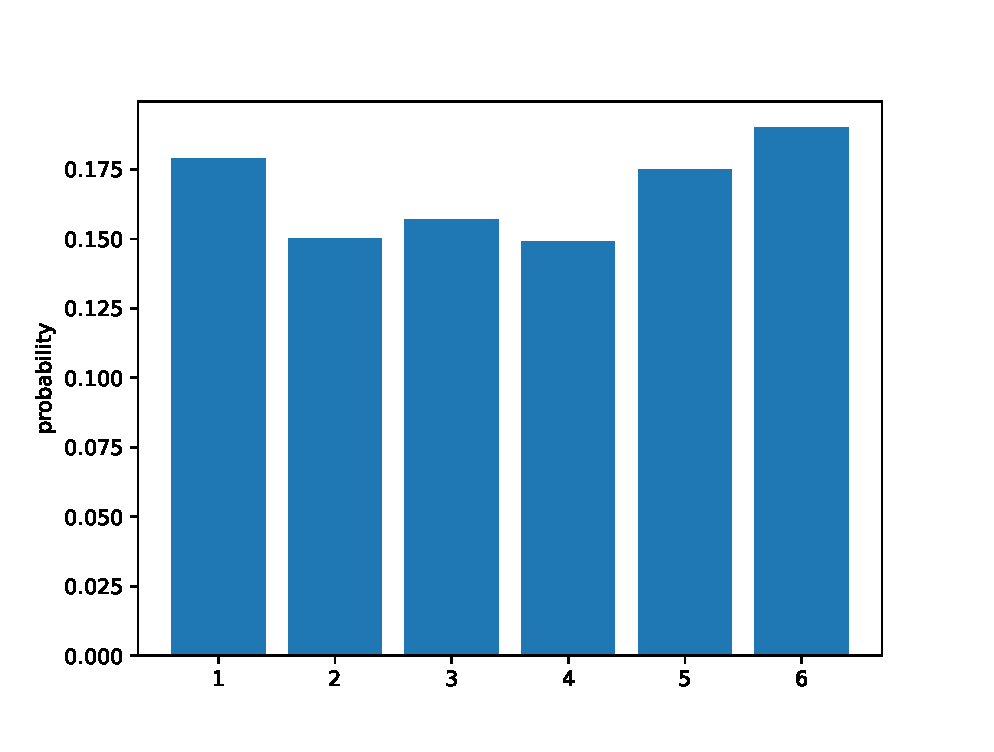
\includegraphics[width=\columnwidth]{./figures/probexm/probexm3.eps}
%	\caption{probability of outcome of biased dice }
%	\label{fig:bts3}
%	\begin{lstlisting}
%	figs/probexm/probexm3.eps
%	\end{lstlisting}
%\end{figure}


   \item The record of a weather station shows that out of the past 250 consecutive days, its weather forecasts were correct 175 times.\\
   (i) What is the probability that on a given day it was correct?\\
(ii) What is the probability that it was not correct on a given day?\\
\solution
Let $X \in \cbrak{0,1}$ be the random variable with 1 denoting correct forecast.
From the given information,
\begin{align}
\pr{X=1} & = \frac{175}{250}
\\
&= 0.7
\\
\pr{X=0} & = 1 - \pr{X=1}
\\
&= 0.3
\end{align}



\item {\em: Random Process}A and B throw a die alternatively till one of them gets a '6' and wins the game. Find their respective probabilities of winning, if A starts first.
\\
\solution
Let X be the random variable representing the number of defective eggs from the ten eggs picked. X follows a  binomial distribution.  Since the probability of an egg being defective is 10\%, substituting n=10, p= 0.1 and k=0 in equation \eqref{eq:exam41_1}, 
probability that there is atleast one defective egg is 
\begin{align}
\pr{X \geq 1}&= 1 - \pr{X=0}  = 1-\brak{0.9}^{10}
\\
&=0.6513215599
\end{align}
The python code for the above problem is,
\begin{lstlisting}
.solutions/20-10/prob/codes/exam42.py
\end{lstlisting}

%
\item To know the opinion of the students about the subject statistics, a survey of 200 students was conducted. The data is recorded in Table \ref{table:1.2.6}
Find the probability that a student chosen at random
\begin{enumerate}
\item likes statistics,
\item  does not like it.
\end{enumerate}
\begin{table}[!ht]
\centering
\begin{tabular}{ |c|c| } 
 \hline
 \textbf{Opinion} &\textbf{Number of students}\\
 \hline
 like  &135\\ 
 \hline
 dislike  &65\\ 
 \hline
\end{tabular}
\caption{}
\label{table:1.2.6}
\end{table}
\solution
Let X be the random variable representing the number of defective eggs from the ten eggs picked. X follows a  binomial distribution.  Since the probability of an egg being defective is 10\%, substituting n=10, p= 0.1 and k=0 in equation \eqref{eq:exam41_1}, 
probability that there is atleast one defective egg is 
\begin{align}
\pr{X \geq 1}&= 1 - \pr{X=0}  = 1-\brak{0.9}^{10}
\\
&=0.6513215599
\end{align}
The python code for the above problem is,
\begin{lstlisting}
.solutions/20-10/prob/codes/exam42.py
\end{lstlisting}

\item  Assume that each born child is equally likely to be a boy or a girl. If a family has two children, what is the conditional probability that both are girls given that\\
(i) the youngest is a girl,\\ 
(ii) at least one is a girl?\\
\solution

	\begin{table}[ht]
    \begin{center}
    	%%%%%%%%%%%%%%%%%%%%%%%%%%%%%%%%%%%%%%%%%%%%%%%%%%%%%%%%%%%%%%%%%%%%%%
%%                                                                  %%
%%  This is the header of a LaTeX2e file exported from Gnumeric.    %%
%%                                                                  %%
%%  This file can be compiled as it stands or included in another   %%
%%  LaTeX document. The table is based on the longtable package so  %%
%%  the longtable options (headers, footers...) can be set in the   %%
%%  preamble section below (see PRAMBLE).                           %%
%%                                                                  %%
%%  To include the file in another, the following two lines must be %%
%%  in the including file:                                          %%
%%        \def\inputGnumericTable{}                                 %%
%%  at the beginning of the file and:                               %%
%%        \input{name-of-this-file.tex}                             %%
%%  where the table is to be placed. Note also that the including   %%
%%  file must use the following packages for the table to be        %%
%%  rendered correctly:                                             %%
%%    \usepackage[latin1]{inputenc}                                 %%
%%    \usepackage{color}                                            %%
%%    \usepackage{array}                                            %%
%%    \usepackage{longtable}                                        %%
%%    \usepackage{calc}                                             %%
%%    \usepackage{multirow}                                         %%
%%    \usepackage{hhline}                                           %%
%%    \usepackage{ifthen}                                           %%
%%  optionally (for landscape tables embedded in another document): %%
%%    \usepackage{lscape}                                           %%
%%                                                                  %%
%%%%%%%%%%%%%%%%%%%%%%%%%%%%%%%%%%%%%%%%%%%%%%%%%%%%%%%%%%%%%%%%%%%%%%



%%  This section checks if we are begin input into another file or  %%
%%  the file will be compiled alone. First use a macro taken from   %%
%%  the TeXbook ex 7.7 (suggestion of Han-Wen Nienhuys).            %%
\def\ifundefined#1{\expandafter\ifx\csname#1\endcsname\relax}


%%  Check for the \def token for inputed files. If it is not        %%
%%  defined, the file will be processed as a standalone and the     %%
%%  preamble will be used.                                          %%
\ifundefined{inputGnumericTable}

%%  We must be able to close or not the document at the end.        %%
	\def\gnumericTableEnd{\end{document}}


%%%%%%%%%%%%%%%%%%%%%%%%%%%%%%%%%%%%%%%%%%%%%%%%%%%%%%%%%%%%%%%%%%%%%%
%%                                                                  %%
%%  This is the PREAMBLE. Change these values to get the right      %%
%%  paper size and other niceties.                                  %%
%%                                                                  %%
%%%%%%%%%%%%%%%%%%%%%%%%%%%%%%%%%%%%%%%%%%%%%%%%%%%%%%%%%%%%%%%%%%%%%%

	\documentclass[12pt%
			  %,landscape%
                    ]{report}
       \usepackage[latin1]{inputenc}
       \usepackage{fullpage}
       \usepackage{color}
       \usepackage{array}
       \usepackage{longtable}
       \usepackage{calc}
       \usepackage{multirow}
       \usepackage{hhline}
       \usepackage{ifthen}

	\begin{document}


%%  End of the preamble for the standalone. The next section is for %%
%%  documents which are included into other LaTeX2e files.          %%
\else

%%  We are not a stand alone document. For a regular table, we will %%
%%  have no preamble and only define the closing to mean nothing.   %%
    \def\gnumericTableEnd{}

%%  If we want landscape mode in an embedded document, comment out  %%
%%  the line above and uncomment the two below. The table will      %%
%%  begin on a new page and run in landscape mode.                  %%
%       \def\gnumericTableEnd{\end{landscape}}
%       \begin{landscape}


%%  End of the else clause for this file being \input.              %%
\fi

%%%%%%%%%%%%%%%%%%%%%%%%%%%%%%%%%%%%%%%%%%%%%%%%%%%%%%%%%%%%%%%%%%%%%%
%%                                                                  %%
%%  The rest is the gnumeric table, except for the closing          %%
%%  statement. Changes below will alter the table's appearance.     %%
%%                                                                  %%
%%%%%%%%%%%%%%%%%%%%%%%%%%%%%%%%%%%%%%%%%%%%%%%%%%%%%%%%%%%%%%%%%%%%%%

\providecommand{\gnumericmathit}[1]{#1} 
%%  Uncomment the next line if you would like your numbers to be in %%
%%  italics if they are italizised in the gnumeric table.           %%
%\renewcommand{\gnumericmathit}[1]{\mathit{#1}}
\providecommand{\gnumericPB}[1]%
{\let\gnumericTemp=\\#1\let\\=\gnumericTemp\hspace{0pt}}
 \ifundefined{gnumericTableWidthDefined}
        \newlength{\gnumericTableWidth}
        \newlength{\gnumericTableWidthComplete}
        \newlength{\gnumericMultiRowLength}
        \global\def\gnumericTableWidthDefined{}
 \fi
%% The following setting protects this code from babel shorthands.  %%
 \ifthenelse{\isundefined{\languageshorthands}}{}{\languageshorthands{english}}
%%  The default table format retains the relative column widths of  %%
%%  gnumeric. They can easily be changed to c, r or l. In that case %%
%%  you may want to comment out the next line and uncomment the one %%
%%  thereafter                                                      %%
\providecommand\gnumbox{\makebox[0pt]}
%%\providecommand\gnumbox[1][]{\makebox}

%% to adjust positions in multirow situations                       %%
\setlength{\bigstrutjot}{\jot}
\setlength{\extrarowheight}{\doublerulesep}

%%  The \setlongtables command keeps column widths the same across  %%
%%  pages. Simply comment out next line for varying column widths.  %%
\setlongtables

\setlength\gnumericTableWidth{%
	53pt+%
	53pt+%
	53pt+%
0pt}
\def\gumericNumCols{3}
\setlength\gnumericTableWidthComplete{\gnumericTableWidth+%
         \tabcolsep*\gumericNumCols*2+\arrayrulewidth*\gumericNumCols}
\ifthenelse{\lengthtest{\gnumericTableWidthComplete > \linewidth}}%
         {\def\gnumericScale{\ratio{\linewidth-%
                        \tabcolsep*\gumericNumCols*2-%
                        \arrayrulewidth*\gumericNumCols}%
{\gnumericTableWidth}}}%
{\def\gnumericScale{1}}

%%%%%%%%%%%%%%%%%%%%%%%%%%%%%%%%%%%%%%%%%%%%%%%%%%%%%%%%%%%%%%%%%%%%%%
%%                                                                  %%
%% The following are the widths of the various columns. We are      %%
%% defining them here because then they are easier to change.       %%
%% Depending on the cell formats we may use them more than once.    %%
%%                                                                  %%
%%%%%%%%%%%%%%%%%%%%%%%%%%%%%%%%%%%%%%%%%%%%%%%%%%%%%%%%%%%%%%%%%%%%%%

\ifthenelse{\isundefined{\gnumericColA}}{\newlength{\gnumericColA}}{}\settowidth{\gnumericColA}{\begin{tabular}{@{}p{53pt*\gnumericScale}@{}}x\end{tabular}}
\ifthenelse{\isundefined{\gnumericColB}}{\newlength{\gnumericColB}}{}\settowidth{\gnumericColB}{\begin{tabular}{@{}p{53pt*\gnumericScale}@{}}x\end{tabular}}
\ifthenelse{\isundefined{\gnumericColC}}{\newlength{\gnumericColC}}{}\settowidth{\gnumericColC}{\begin{tabular}{@{}p{53pt*\gnumericScale}@{}}x\end{tabular}}

\begin{tabular}[c]{%
	b{\gnumericColA}%
	b{\gnumericColB}%
	b{\gnumericColC}%
	}

%%%%%%%%%%%%%%%%%%%%%%%%%%%%%%%%%%%%%%%%%%%%%%%%%%%%%%%%%%%%%%%%%%%%%%
%%  The longtable options. (Caption, headers... see Goosens, p.124) %%
%	\caption{The Table Caption.}             \\	%
% \hline	% Across the top of the table.
%%  The rest of these options are table rows which are placed on    %%
%%  the first, last or every page. Use \multicolumn if you want.    %%

%%  Header for the first page.                                      %%
%	\multicolumn{3}{c}{The First Header} \\ \hline 
%	\multicolumn{1}{c}{colTag}	%Column 1
%	&\multicolumn{1}{c}{colTag}	%Column 2
%	&\multicolumn{1}{c}{colTag}	\\ \hline %Last column
%	\endfirsthead

%%  The running header definition.                                  %%
%	\hline
%	\multicolumn{3}{l}{\ldots\small\slshape continued} \\ \hline
%	\multicolumn{1}{c}{colTag}	%Column 1
%	&\multicolumn{1}{c}{colTag}	%Column 2
%	&\multicolumn{1}{c}{colTag}	\\ \hline %Last column
%	\endhead

%%  The running footer definition.                                  %%
%	\hline
%	\multicolumn{3}{r}{\small\slshape continued\ldots} \\
%	\endfoot

%%  The ending footer definition.                                   %%
%	\multicolumn{3}{c}{That's all folks} \\ \hline 
%	\endlastfoot
%%%%%%%%%%%%%%%%%%%%%%%%%%%%%%%%%%%%%%%%%%%%%%%%%%%%%%%%%%%%%%%%%%%%%%

\hhline{|-|-~}
	 \multicolumn{1}{|p{\gnumericColA}|}%
	{\gnumericPB{\centering}\gnumbox{Mark}}
	&\multicolumn{1}{p{\gnumericColB}|}%
	{\gnumericPB{\centering}\gnumbox{Frequency}}
	&
\\
\hhline{|--|~}
	 \multicolumn{1}{|p{\gnumericColA}|}%
	{\gnumericPB{\centering}\gnumbox{2}}
	&\multicolumn{1}{p{\gnumericColB}|}%
	{\gnumericPB{\centering}\gnumbox{1}}
	&
\\
\hhline{|--|~}
	 \multicolumn{1}{|p{\gnumericColA}|}%
	{\gnumericPB{\centering}\gnumbox{3}}
	&\multicolumn{1}{p{\gnumericColB}|}%
	{\gnumericPB{\centering}\gnumbox{2}}
	&
\\
\hhline{|--|~}
	 \multicolumn{1}{|p{\gnumericColA}|}%
	{\gnumericPB{\centering}\gnumbox{4}}
	&\multicolumn{1}{p{\gnumericColB}|}%
	{\gnumericPB{\centering}\gnumbox{3}}
	&
\\
\hhline{|--|~}
	 \multicolumn{1}{|p{\gnumericColA}|}%
	{\gnumericPB{\centering}\gnumbox{5}}
	&\multicolumn{1}{p{\gnumericColB}|}%
	{\gnumericPB{\centering}\gnumbox{2}}
	&
\\
\hhline{|--|~}
	 \multicolumn{1}{|p{\gnumericColA}|}%
	{\gnumericPB{\centering}\gnumbox{6}}
	&\multicolumn{1}{p{\gnumericColB}|}%
	{\gnumericPB{\centering}\gnumbox{3}}
	&
\\
\hhline{|--|~}
	 \multicolumn{1}{|p{\gnumericColA}|}%
	{\gnumericPB{\centering}\gnumbox{7}}
	&\multicolumn{1}{p{\gnumericColB}|}%
	{\gnumericPB{\centering}\gnumbox{3}}
	&
\\
\hhline{|--|~}
	 \multicolumn{1}{|p{\gnumericColA}|}%
	{\gnumericPB{\centering}\gnumbox{9}}
	&\multicolumn{1}{p{\gnumericColB}|}%
	{\gnumericPB{\centering}\gnumbox{4}}
	&
\\
\hhline{|--|~}
	 \multicolumn{1}{|p{\gnumericColA}|}%
	{\gnumericPB{\centering}\gnumbox{10}}
	&\multicolumn{1}{p{\gnumericColB}|}%
	{\gnumericPB{\centering}\gnumbox{2}}
	&
\\
\hhline{|-|-|~}
\end{tabular}

\ifthenelse{\isundefined{\languageshorthands}}{}{\languageshorthands{\languagename}}
\gnumericTableEnd

  \caption{Marks obtained by students}
   \label{table:statsex_23table1}
   \end{center}	
\end{table}

As we can see from table \ref{table:statsex_23table1}, 9 occurs the maximum number of times.\\
Thus Mode = 9.




\item  An instructor has a question bank consisting of 300 easy True / False questions,
200 difficult True / False questions, 500 easy multiple choice questions and 400 difficult multiple choice questions. If a question is selected at random from the question bank, what is the probability that it will be an easy question given that it is a multiple choice question?\\
\solution
From the given information, using the fact that $A,B$ are independent,
\begin{align}
\pr{A+B} &= \pr{A}+\pr{B}-\pr{AB}
\\
&= \pr{A} + \pr{B-AB} 
\\
&= \pr{A} + \pr{A'B}
\\
&= \pr{A} + \pr{A'}\pr{B}
\\
&= \pr{A} + \pr{A'}\brak{1-\pr{B'}}
\\
&= \pr{A} + \pr{A'}-\pr{A'}\pr{B'}
\\
&=1 - \pr{A'}\pr{B'}
\end{align}


\item Two cards are drawn at random and without replacement from a pack of 52 playing cards. Find the probability that both the cards are black.\\
\solution
Let $X_1,X_2 \in \cbrak{0,1}$ represent the colour, where 0 denotes black and 1 denotes red.  From the given information,
\begin{align}
\pr{X_1 = 0} &= \frac{26}{52}= \frac{1}{2}
\\
\pr{X_2 = 0|X_1 = 0} &= \frac{25}{51}
\end{align}
Then,
\begin{multline}
\pr{X_1=0,X_2=0} 
\\
= \pr{X_2 = 0|X_1 = 0}\pr{X_1 = 0}
 = \frac{25}{102}
\end{multline}

\item Two balls are drawn at random with replacement from a box containing 10 black and 8 red balls. Find the probability that\\
(i) both balls are red.\\
(ii) first ball is black and second is red.\\
(iii) one of them is black and other is red.\\
\solution
Let X be the random variable representing the number of defective eggs from the ten eggs picked. X follows a  binomial distribution.  Since the probability of an egg being defective is 10\%, substituting n=10, p= 0.1 and k=0 in equation \eqref{eq:exam41_1}, 
probability that there is atleast one defective egg is 
\begin{align}
\pr{X \geq 1}&= 1 - \pr{X=0}  = 1-\brak{0.9}^{10}
\\
&=0.6513215599
\end{align}
The python code for the above problem is,
\begin{lstlisting}
.solutions/20-10/prob/codes/exam42.py
\end{lstlisting}


\item Probability of solving specific problem independently by A and B are $\frac{1}{2}$
and $\frac{1}{3}$ respectively. If both try to solve the problem independently, find the probability that\\
(i) the problem is solved \\
(ii) exactly one of them solves the problem.\\
\solution
Let X be the random variable representing the number of defective eggs from the ten eggs picked. X follows a  binomial distribution.  Since the probability of an egg being defective is 10\%, substituting n=10, p= 0.1 and k=0 in equation \eqref{eq:exam41_1}, 
probability that there is atleast one defective egg is 
\begin{align}
\pr{X \geq 1}&= 1 - \pr{X=0}  = 1-\brak{0.9}^{10}
\\
&=0.6513215599
\end{align}
The python code for the above problem is,
\begin{lstlisting}
.solutions/20-10/prob/codes/exam42.py
\end{lstlisting}

\item (i) A lot of 20 bulbs contain 4 defective ones. One bulb is drawn at random from the lot.
What is the probability that this bulb is defective?\\
(ii) Suppose the bulb drawn in (i) is not defective and is not replaced. Now one bulb
is drawn at random from the rest. What is the probability that this bulb is not
defective ?
\\
\solution
Let X be the random variable representing the number of defective eggs from the ten eggs picked. X follows a  binomial distribution.  Since the probability of an egg being defective is 10\%, substituting n=10, p= 0.1 and k=0 in equation \eqref{eq:exam41_1}, 
probability that there is atleast one defective egg is 
\begin{align}
\pr{X \geq 1}&= 1 - \pr{X=0}  = 1-\brak{0.9}^{10}
\\
&=0.6513215599
\end{align}
The python code for the above problem is,
\begin{lstlisting}
.solutions/20-10/prob/codes/exam42.py
\end{lstlisting}

\item 12 defective pens are accidentally mixed with 132 good ones. It is not possible to just
look at a pen and tell whether or not it is defective. One pen is taken out at random from
this lot. Determine the probability that the pen taken out is a good one.
\\
\solution
Let X be the random variable representing the number of defective eggs from the ten eggs picked. X follows a  binomial distribution.  Since the probability of an egg being defective is 10\%, substituting n=10, p= 0.1 and k=0 in equation \eqref{eq:exam41_1}, 
probability that there is atleast one defective egg is 
\begin{align}
\pr{X \geq 1}&= 1 - \pr{X=0}  = 1-\brak{0.9}^{10}
\\
&=0.6513215599
\end{align}
The python code for the above problem is,
\begin{lstlisting}
.solutions/20-10/prob/codes/exam42.py
\end{lstlisting}

\item Gopi buys a fish from a shop for his aquarium. The
shopkeeper takes out one fish at random from a
tank containing 5 male fish and 8 female fish (see
Fig. \ref{fig:prob_121}). What is the probability that the fish taken
out is a male fish?
\begin{figure}[!ht]
\centering
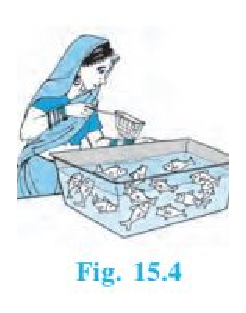
\includegraphics[width=\columnwidth]{./prob/figs/woman.eps}
\caption{}
\label{fig:prob_121}
\end{figure}
\\
\solution
Let X be the random variable representing the number of defective eggs from the ten eggs picked. X follows a  binomial distribution.  Since the probability of an egg being defective is 10\%, substituting n=10, p= 0.1 and k=0 in equation \eqref{eq:exam41_1}, 
probability that there is atleast one defective egg is 
\begin{align}
\pr{X \geq 1}&= 1 - \pr{X=0}  = 1-\brak{0.9}^{10}
\\
&=0.6513215599
\end{align}
The python code for the above problem is,
\begin{lstlisting}
.solutions/20-10/prob/codes/exam42.py
\end{lstlisting}
    
\item A lot consists of 144 ball pens of which 20 are defective and the others are good. Nuri will buy a pen if it is good, but will not buy if it is defective. The shopkeeper draws one pen at random and gives it to her. What is the probability that\\
(i) She will buy it ?\\
(ii) She will not buy it ?
\\
\solution
Let X be the random variable representing the number of defective eggs from the ten eggs picked. X follows a  binomial distribution.  Since the probability of an egg being defective is 10\%, substituting n=10, p= 0.1 and k=0 in equation \eqref{eq:exam41_1}, 
probability that there is atleast one defective egg is 
\begin{align}
\pr{X \geq 1}&= 1 - \pr{X=0}  = 1-\brak{0.9}^{10}
\\
&=0.6513215599
\end{align}
The python code for the above problem is,
\begin{lstlisting}
.solutions/20-10/prob/codes/exam42.py
\end{lstlisting}


\item A bag contains 5 red balls and some blue balls. If the probability of drawing a blue ball is double that of a red ball, determine the number of blue balls in the bag.
\\
\solution
Let X be the random variable representing the number of defective eggs from the ten eggs picked. X follows a  binomial distribution.  Since the probability of an egg being defective is 10\%, substituting n=10, p= 0.1 and k=0 in equation \eqref{eq:exam41_1}, 
probability that there is atleast one defective egg is 
\begin{align}
\pr{X \geq 1}&= 1 - \pr{X=0}  = 1-\brak{0.9}^{10}
\\
&=0.6513215599
\end{align}
The python code for the above problem is,
\begin{lstlisting}
.solutions/20-10/prob/codes/exam42.py
\end{lstlisting}

\item A box contains 12 balls out of which x are black. If one ball is drawn at random from the box,what is the probability that it will be a black ball?\\
If 6 more black balls are put in the box, the probability of drawing a black ball is now double of what it was before. Find x.
\\
\solution
Let X be the random variable representing the number of defective eggs from the ten eggs picked. X follows a  binomial distribution.  Since the probability of an egg being defective is 10\%, substituting n=10, p= 0.1 and k=0 in equation \eqref{eq:exam41_1}, 
probability that there is atleast one defective egg is 
\begin{align}
\pr{X \geq 1}&= 1 - \pr{X=0}  = 1-\brak{0.9}^{10}
\\
&=0.6513215599
\end{align}
The python code for the above problem is,
\begin{lstlisting}
.solutions/20-10/prob/codes/exam42.py
\end{lstlisting}

\end{enumerate}
%\end{document}
    

\section{Stochastic Geometry}
Suppose you drop a die at random on the rectangular region shown in Fig. \ref{fig:chapters/uniform/1/}. What is the probability that it will land inside the circle with diameter 1m?
\renewcommand{\theequation}{\theenumi}
\renewcommand{\thefigure}{\theenumi}
\begin{enumerate}[label=\thesection.\arabic*.,ref=\thesection.\theenumi]
\numberwithin{equation}{enumi}
\numberwithin{figure}{enumi}
%
\item 
\begin{figure}[!ht]
\centering
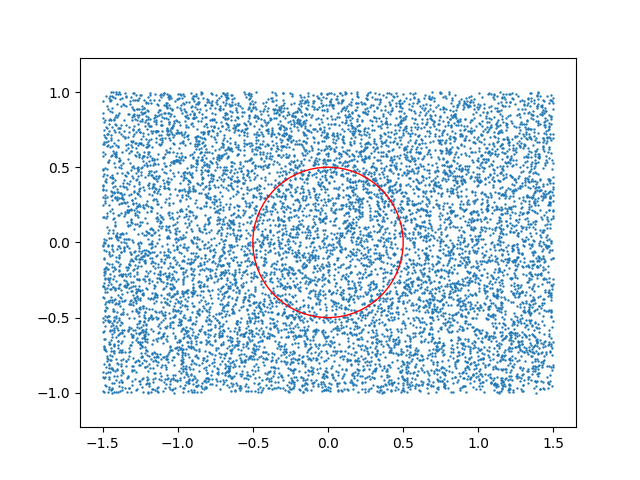
\includegraphics[width=\columnwidth]{./figs/stochastic/rectangle.png}
\caption{}
\label{fig:chapters/uniform/1/}
\end{figure}
%\\
%\solution
In Fig. \ref{fig:chapters/uniform/1/}, the sample size $S$ is the area of the rectangle given by 
\begin{align}
S=3\times 2=6 m^2
\end{align}
The event size is the area of the circle given by 
\begin{align}
E = \pi\brak{\frac{1}{2}}^2=\frac{\pi}{4} m^2 
\end{align}
The probabilty of the dice landing in the circle is
\begin{align}
\pr{E} = \frac{E}{S} = \frac{\pi}{24}
\label{eq:chapters/uniform/1/prob}
\end{align}
%
\item The python code is available in 
\begin{lstlisting}
/codes/stochastic/rect.py
\end{lstlisting}
The python code generates 10,000 points uniformly within the rectangle of dimensions $3 \times 2$ and checks for the number of points within the circle of radius 0.5.  The ratio of these is close to $\frac{\pi}{24}$.  Note that each time the code is run, the ratio will change, but will still be close to $\frac{\pi}{24}$.



\end{enumerate}

\section{Transformation of Variables}
\renewcommand{\theequation}{\theenumi}
\renewcommand{\thefigure}{\theenumi}

%\subsection{Independence}
\subsection{Using Definition}
\begin{enumerate}[label=\thesubsection.\arabic*.,ref=\thesubsection.\theenumi]
\numberwithin{equation}{enumi}
\numberwithin{figure}{enumi}

%
\item
Let $X_1 \sim  \gauss{0}{1}$ and $X_2 \sim  \gauss{0}{1}$. Plot the CDF and PDF of
%
\begin{equation}
V = X_1^2 + X_2^2 
\end{equation}
%
% \solution The following code generates the simulated CDF in Fig. \ref{fig:probman_trans_cdf_V}
% %
% \begin{figure}[!ht]
% \centering
% 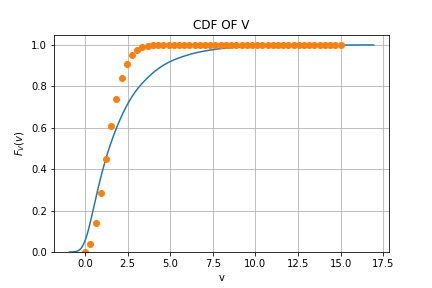
\includegraphics[width=\columnwidth]{figs/trans/cdf_V.png}
% \caption{CDF of $V$}
% \label{fig:probman_trans_cdf_V}
% \end{figure}
% %
% and the PDF in Fig. \ref{fig:probman_trans_pdf_V}
% %
% \begin{figure}[!ht]
% \centering
% 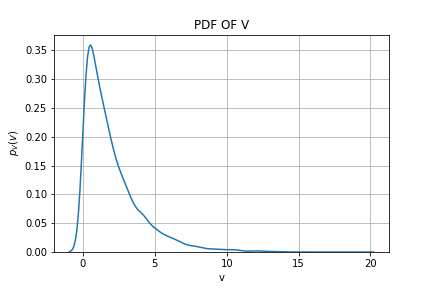
\includegraphics[width=\columnwidth]{figs/trans/pdf_V.png}
% \caption{PDF of $V$}
% \label{fig:probman_trans_pdf_V}
% \end{figure}
%

\item
If
%
\begin{equation}
F_{V}(x) = 
\begin{cases}
1 - e^{-\alpha x} & x \geq 0 \\
0 & x < 0,
\end{cases}
\label{eq:probman_F_V_alpha}
\end{equation}
%
find $\alpha$.

%
\item
\label{ch3_raleigh_sim}
Plot the CDF and PDf of
%
\begin{equation}
A = \sqrt{V}
\end{equation}
%

%
\item
Find an expression for $F_{A}(x)$ using the definition. Plot this expression and compare with the result of problem \ref{ch3_raleigh_sim}. 
\\
\solution 
% Given,
% \begin{align}
% A = \sqrt{V}
% \end{align}

\begin{align} 
F_A(x) &= \pr{A \le x} = \pr{\sqrt{V} \le x}
\\
&= \pr{V \le x^2} = F_V\brak{x^2}
\end{align}
%
From \label{eq:probman_F_V_alpha}, 
\begin{align} 
F_V\brak{x^2} = 
\begin{cases}
1 - e^{-\alpha x^2} & x \geq 0 \\
0 & x < 0,
\end{cases}
\end{align}
%
Substituting 

\begin{align}
\alpha = \frac{1}{2}
\end{align}

%
\begin{align} 
F_V\brak{x^2} = 
\begin{cases}
1 - e^{- \frac{x^2}{2}} & x \geq 0 \\
0 & x < 0,
\end{cases}
\end{align}
%
\item
Find an expression for $p_{A}(x)$.
\\
\solution
The PDf is obtained as
\begin{align}
f_V\brak{x^2} &= \frac{d}{dx}F_V\brak{x^2}
\\
&=
\begin{cases}
x e^{- \frac{x^2}{2}} & x \geq 0 \\
0 & x < 0,
\end{cases}
\end{align}
%
\end{enumerate}

%
\subsection{Using Jacobian}
%
\begin{enumerate}[label=\thesubsection.\arabic*.,ref=\thesubsection.\theenumi]
\numberwithin{equation}{enumi}
\numberwithin{figure}{enumi}

\item
Evaluate the joint PDF of $X_1,X_2$,  given by
%
\begin{equation}
p_{X_1,X_2}(x_1,x_2) = p_{X_1}\brak{x_1}p_{X_2}\brak{x_2}
\end{equation}
%

%
\item
Let 
\begin{align}
 X_1 = \sqrt{V}\cos \theta
\\
 X_2 = \sqrt{V} \sin \theta.
\end{align}
Evaluate the Jacobian 
%
\begin{equation}
J =
\begin{vmatrix}
\frac{\partial x_1}{\partial v} & \frac{\partial x_2}{\partial v} \\
\frac{\partial x_1}{\partial \theta} & \frac{\partial x_2}{\partial \theta} 
\end{vmatrix}
\end{equation}
%

%
\item
Find
%
\begin{equation}
p_{V,\Theta}\brak{v,\theta} = \abs{J}p_{X_1,X_2}\brak{x_1,x_2}
\end{equation}
%

%
\item
Find $p_{V}(v)$.  

%
%
\item
Find $p_{\Theta}(\theta)$.  

%
\item
Are $Y$ and $\Theta$ independent?

\item
Find $p_{A}(x)$ using the Jacobian.

%%
%\item
%Let $X_1 \sim  \gauss{2}{1}$ and $X_2 \sim  \gauss{3}{1}$. Find $E\sbrak{X_1X_2}$.  Try with different mean and variances. Comment.
%
%

%\section{The Transform Domain}
%\item
%Find the MGF of $X \sim \gauss{\mu}{\sigma^2}$. 
%
%\item
%Find the MGF of $Y$.
%
%%
%\item
%Find the PDF of $Y$ by inverting the MGF.
%
%%
\end{enumerate}

%
\section{Conditional Probability}
\begin{enumerate}[label=\thesection.\arabic*.,ref=\thesection.\theenumi]
\numberwithin{equation}{enumi}
\numberwithin{figure}{enumi}
%%
\item
\label{ch4_sim}
Plot 
\begin{equation}
P_e = \pr{\hat{X} = -1|X=1}
\end{equation}
%
for 
\begin{equation}
Y = AX+N,
\end{equation}
where $A$ is Raleigh with $E\sbrak{A^2} = \gamma, N \sim \gauss{0}{1}, X \in \brak{-1,1}$ for $0 \le \gamma \le 10$ dB.

%
\item
Assuming that $N$ is a constant, find an expression for $P_e$.  Call this $P_e(N)$

%
\item
%
\label{ch4_anal}
For a function $g$,
\begin{equation}
E\sbrak{g(X)} = \int_{-\infty}^{\infty}g(x)p_{X}(x)\, dx
\end{equation}
%
Find $P_e = E\sbrak{P_e(N)}$.

%
\item
Plot $P_e$ in problems \ref{ch4_sim} and \ref{ch4_anal} on the same graph w.r.t $\gamma$.  Comment.

\end{enumerate}

%%
\section{Two Dimensions}
\begin{enumerate}[label=\thesection.\arabic*.,ref=\thesection.\theenumi]
    \numberwithin{equation}{enumi}
    \numberwithin{figure}{enumi}
    %%
    \item Let 
    \begin{equation}
    \mbf{y} = A\mbf{x} + \mbf{n},
    \end{equation}
    where 
    \begin{align}
    x &\in \brak{\mbf{s}_0,\mbf{s}_1}, 
    \mbf{s}_0 = 
    \begin{pmatrix}
    1 
    \\
    0
    \end{pmatrix},
    \mbf{s}_1 = 
    \begin{pmatrix}
    0 
    \\
    1
    \end{pmatrix}
    \\
    \mbf{n} &= 
    \begin{pmatrix}
    n_1
    \\
    n_2
    \end{pmatrix},
    n_1,n_2 \sim \gauss{0}{1}.
    \end{align}
    %
    \item
    \label{ch5_fsk}
    Plot 
    %
    \begin{equation}
    \mbf{y}|\mbf{s}_0 \text{ and } \mbf{y}|\mbf{s}_1
    \end{equation}
    %
    on the same graph using a scatter plot.
    %
    \solution The following python code plots the scatter plot when $\mbf{x} = \mbf{s}_0$ and $\mbf{x} = \mbf{s}_1$ in Fig. \ref{fig:scatter_plt_y}
    \begin{lstlisting}
    codes/twoD/scatter_plot.py
    \end{lstlisting}
    \begin{figure}
    \centering
    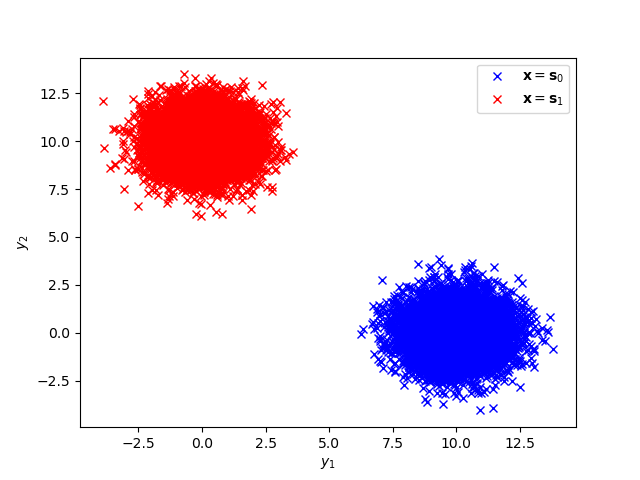
\includegraphics[width=\columnwidth]{./figs/twoD/scatter_plot.png}
    \caption{Scatter plot of $\vec{y}$ for $A = 10$}
    \label{fig:scatter_plt_y}
    \end{figure}
    %
    %
    \item
    For the above problem, find a decision rule for detecting the symbols $\mbf{s}_0 $ and $\mbf{s}_1$.
    \\
    \solution The multivariate Gaussian distribution is defined as
    %
    \begin{multline}
    \label{eq:multivariate}
    p_{\mathbf{x}}(x_1,\dots,x_k)
    \\
    =\frac{1}{\sqrt{\brak{2\pi}^k\abs{\mbf{\Sigma}}}}\exp\cbrak{-\frac{1}{2}\brak{\mathbf{x}-\mbf{\mu}}^T\mbf{\Sigma}^{-1}\brak{\mathbf{x}-\mbf{\mu}}}
    \end{multline}
    %
    where $\mbf{\mu}$ is the mean vector, $\mbf{\Sigma} = E\sbrak{\brak{\mathbf{x}-\mbf{\mu}}\brak{\mathbf{x}-\mbf{\mu}}^T}$ is the covariance matrix and $\abs{\mbf{\Sigma}}$ is the determinant of $\mbf{\Sigma}$.
    For a bivariate gaussian distribution,
    {\small
    \begin{multline}
    \label{eq:bivariate}
    p(x,y)= \frac{1}{2\pi \sigma_x\sigma_y\sqrt{1-\rho^2}}\exp\lsbrak{-\frac{1}{2\brak{1-\rho^2}}}
    \\
    \times \rsbrak{\cbrak{\frac{\brak{x-\mu_x}^2}{\sigma_x^2}+\frac{\brak{y-\mu_y}^2}{\sigma_y^2}-\frac{2\rho\brak{x-\mu_x}\brak{y-\mu_y}}{\sigma_x\sigma_y}}}
    \end{multline}
    }
    %
    where
    %
    \begin{align}
    %\mbf{\mu}=
    &\mbf{\mu}=
    \begin{pmatrix*}
    \mu_x \\
    \mu_y
    \end{pmatrix*},
    \mbf{\Sigma} = 
    \begin{pmatrix*}%[r]
    \sigma_x^2 & \rho\sigma_x\sigma_y \\
    \rho\sigma_x\sigma_y & \sigma_y^2
    \end{pmatrix*},\\
    &\rho = \frac{E\sbrak{\brak{x - \mu_x}\brak{y-\mu_y}}}{\sigma_x\sigma_y}.
    \end{align}
    %
    \begin{align}
        \mbf{y}|s_0 &= 
        \begin{pmatrix}
        A+n_1 \\
        n_2
        \end{pmatrix}\\
        \mbf{y}|s_1 &=  
        \begin{pmatrix}
        n_1 \\
        A+n_2
        \end{pmatrix}
        \end{align}
        Substituting these values in (\ref{eq:bivariate}),
        \begin{multline}
        \label{gauss_mutl_var1}
        p\brak{\mbf{y}|s_0} = \frac{1}{2\pi\sigma_{y_1}\sigma_{y_2}\sqrt{1-\rho_1^2}}\exp\lsbrak{-\frac{1}{2\brak{1-\rho_1^2}}}
        \\
        \times \rsbrak{\cbrak{\frac{\brak{y_1-A}^2}{\sigma_{y_1}^2}+\frac{\brak{y_2}^2}{\sigma_{y_2}^2}-\frac{2\rho_1\brak{y_1-A}\brak{y_2}}{\sigma_{y_1}\sigma_{y_2}}}}
        \end{multline}
        \begin{multline}
        \label{gauss_mutl_var2}
        p\brak{\mbf{y}|s_1} = \frac{1}{2\pi\sigma_{y_1}\sigma_{y_2}\sqrt{1-\rho_2^2}}\exp\lsbrak{-\frac{1}{2\brak{1-\rho_2^2}}}
        \\
        \times \rsbrak{\cbrak{\frac{\brak{y_1}^2}{\sigma_{y_1}^2}+\frac{\brak{y_2-A}^2}{\sigma_{y_2}^2}-\frac{2\rho_2\brak{y_1}\brak{y_2-A}}{\sigma_{y_1}\sigma_{y_2}}}}
        \end{multline}
        where,
        \begin{align}
        \label{rho_sig_val}
        \rho_1 = E[(y_1-A)(y_2)] &= E[n_1 n_2] = 0, \nonumber \\
        \rho_2 = E[(y_1)(y_2-A)] &= E[n_1 n_2] = 0, \nonumber \\
        \sigma_{y_1} = \sigma_{y_2} &= 1
        \end{align}
        For equiprobably symbols, the MAP criterion is defined as
        %
        \begin{align}
        \label{eq:map_bfsk_dec}
        p\brak{\vec{y}|s_0} &\dec{s_0}{s_1} p\brak{\vec{y}|s_1}
        \end{align}
        Using (\ref{gauss_mutl_var1}) and (\ref{gauss_mutl_var2}) and substituting the values from (\ref{rho_sig_val}),  we get
        \begin{align}
        (y_1 -A)^2 + y_2^2 \dec{s_1}{s_0} y_1^2 + (y_2 - A)^2
        \end{align}
        On simplifying, we get the decision rule is
        \begin{align}
        \label{eq:decision_rule}
        y_1 \dec{s_0}{s_1} y_2
        \end{align}
    %    
    \item
    Plot 
    \begin{equation} 
    P_e = \pr{\hat{\mbf{x}} = \mbf{s}_1|\mbf{x} = \mbf{s}_0}
    \end{equation}
    with respect to the SNR from 0 to 10 dB.
    \\
    \solution
    \begin{figure}
        \centering
        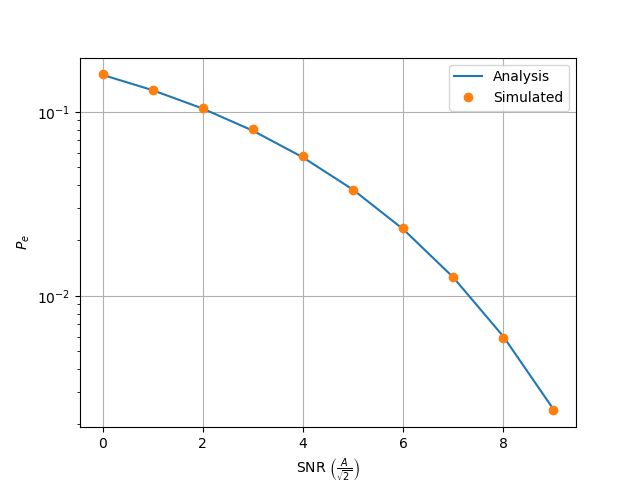
\includegraphics[width=\columnwidth]{./figs/twoD/ber_snr_plot.png}
        \caption{$P_e$ with respect to SNR from 0 to 10 dB}
        \label{fig:ber_snr_plot}
        \end{figure}
    %
    \item
    Obtain an expression for $P_e$. Verify this by comparing the theory and simulation plots on the same graph.
    \\
    \solution 
    \begin{align}
    P_e = \pr{\hat{\mbf{x}} = \mbf{s}_1|\mbf{x} = \mbf{s}_0}
    \end{align}
    Given that $\mbf{s}_0$ was transmitted, the received signal is
    \begin{align}
    \mbf{y}|\mbf{s}_0 = \begin{pmatrix} A \\ 0 \end{pmatrix} + \begin{pmatrix} n_1 \\ n_2 \end{pmatrix}
    \end{align}
    From (\ref{eq:decision_rule}), the probability of error is given by 
    \begin{align}
    P_e &= \pr{y_1 < y_2 |\mbf{s}_0} = \pr{A+n_1 < n_2}\\
    &= \pr{n_2 - n_1 > A}
    \end{align}
    Note that $n_2 - n_1 \sim \gauss{0}{2}$. Thus,
    \begin{align}
    P_e &= \pr{\sqrt{2}w > A}\\
    \pr{w > \dfrac{A}{\sqrt{2}}}\\
    \Rightarrow P_e &= \qfunc{\frac{A}{\sqrt{2}}}
    \end{align}
    where $w \sim \gauss{0}{1}$. The following code plots the $P_e$ curve in Fig. (\ref{fig:ber_snr_plot}).
    \begin{lstlisting}
    codes/twoD/ber_snr_plot.py
    \end{lstlisting}
    %
    \end{enumerate}

    % \begin{enumerate}[label=\thesection.\arabic*.,ref=\thesection.\theenumi]


% \numberwithin{equation}{enumi}
% \numberwithin{figure}{enumi}
% %%
% \item Let 
% \begin{equation}
% \mbf{y} = A\mbf{x} + \mbf{n},
% \end{equation}
% where 
% \begin{align}
% x &\in \brak{\mbf{s}_0,\mbf{s}_1}, 
% \mbf{s}_0 = 
% \begin{pmatrix}
% 1 
% \\
% 0
% \end{pmatrix},
% \mbf{s}_1 = 
% \begin{pmatrix}
% 0 
% \\
% 1
% \end{pmatrix}
% \\
% \mbf{n} &= 
% \begin{pmatrix}
% n_1
% \\
% n_2
% \end{pmatrix},
% n_1,n_2 \sim \gauss{0}{1}.
% \end{align}
% %
% \item
% \label{ch5_fsk}
% Plot 
% %
% \begin{equation}
% \mbf{y}|\mbf{s}_0 \text{ and } \mbf{y}|\mbf{s}_1
% \end{equation}
% %
% on the same graph using a scatter plot.

% %
% \item
% For the above problem, find a decision rule for detecting the symbols $\mbf{s}_0 $ and $\mbf{s}_1$.

% %
% \item
% Plot 
% \begin{equation} 
% P_e = \pr{\hat{\mbf{x}} = \mbf{s}_1|\mbf{x} = \mbf{s}_0}
% \end{equation}
% with respect to the SNR from 0 to 10 dB.

% %
% \item
% Obtain an expression for $P_e$. Verify this by comparing the theory and simulation plots on the same graph.

% %
% \end{enumerate}

%%
\section{Transform Domain: Moment Generating Function}
Let $X \sim \gauss{\mu}{\sigma^2}$.

\begin{enumerate}[label=\thesection.\arabic*.,ref=\thesection.\theenumi]
\numberwithin{equation}{enumi}
\numberwithin{figure}{enumi}
%%
\item
Find $M_{X}\brak{s} = E\sbrak{e^{-sX}}$.
\\
\solution The MGF of $X$ is
%
\begin{align}
M_{X}(s) &=\int_{-\infty}^{\infty}e^{-s X}p_{X}(x) dx 
\\
&=e^{-s\mu}e^{-\frac{s^2\sigma^2}{2}}
\label{eq:probman_mgf_X}
\end{align}
%
\item
Let 
%
\begin{equation}
N = n_1 - n_2, \quad   n_1,n_2 \sim \gauss{0}{1}.
\end{equation}
%
Find $M_{N}(s)$, assuming that $n_1$ and $n_2$ are independent.
\\
\solution Substituting from \eqref{eq:probman_mgf_X} and using independence,
\begin{align}
M_N(s)&=E[e^{-(n_1-n_2)s}]=M_{n_1}(s) M_{n_2}(-s)
\\
&= e^{-s^2\sigma^2} = e^{-s^2} \quad \brak{\because \sigma = 1}
\label{eq:probman_mgf_N}
\end{align}
%
\item
Show that $N$ is Gaussian. Find its mean and variance.  Comment.
\\
\solution From \eqref{eq:probman_mgf_N} and \eqref{eq:probman_mgf_X}, it is obvious that $X \sim \gauss{0}{2}$.  Thus,
%
the difference of two Gaussian random variables is also a Gaussian random variable.

\end{enumerate}

%%
\section{Uniform to Other: Quantile function}
\begin{enumerate}[label=\thesection.\arabic*.,ref=\thesection.\theenumi]
\numberwithin{equation}{enumi}
\numberwithin{figure}{enumi}
%%
%
%
\item
Generate samples of 
%
\begin{equation}
V = -2\ln\brak{1-U}
\label{eq:probman_V_cdf_sim}
\end{equation}
%
and plot its CDF.  Comment.
\\
\solution
Let X be the random variable representing the number of defective eggs from the ten eggs picked. X follows a  binomial distribution.  Since the probability of an egg being defective is 10\%, substituting n=10, p= 0.1 and k=0 in equation \eqref{eq:exam41_1}, 
probability that there is atleast one defective egg is 
\begin{align}
\pr{X \geq 1}&= 1 - \pr{X=0}  = 1-\brak{0.9}^{10}
\\
&=0.6513215599
\end{align}
The python code for the above problem is,
\begin{lstlisting}
.solutions/20-10/prob/codes/exam42.py
\end{lstlisting}


%
\item
Generate the Rayleigh distribution from Uniform. Verify your result through graphical plots.

\end{enumerate}


%\section{Sum of i.i.d random variables}
%\input{./chapters/conv.tex}


\end{document}


